\documentclass[12pt]{article}
 
\usepackage[margin=1in]{geometry} 
\usepackage{amsmath,amsthm,amssymb,graphicx,mathtools,tikz,float,mathrsfs,multicol,textcomp,gensymb,extarrows,dsfont,tikz-cd,subcaption,enumerate,cancel}
\usepackage[urlcolor=blue]{hyperref}
\hypersetup{
     colorlinks   = true,
     citecolor    = gray
} % Lime green, really?! Not only is that a sore sight, lime green has been an enemy of mine since 2007.
\usetikzlibrary{positioning}
\newcommand{\n}{\mathbb{N}}
\newcommand{\z}{\mathbb{Z}}
\newcommand{\q}{\mathbb{Q}}
\newcommand{\cx}{\mathbb{C}}
\newcommand{\real}{\mathbb{R}}
\newcommand{\field}{\mathbb{F}}
\newcommand{\h}{\mathbb{H}}
\newcommand{\m}{\mathbb{M}}
\newcommand{\p}{\mathbb{P}}
\newcommand{\ita}[1]{\textit{#1}}
\newcommand{\oneton}[1]{\{1,\dotsc,#1\}}
\newcommand\idea[1]{\begin{gather*}#1\end{gather*}}
\newcommand\proofs[1]{\begin{proof}#1\end{proof}}
\newcommand\inv[1]{#1^{-1}}
\newcommand\paren[1]{\left( #1 \right)}
\newcommand\setb[1]{\left \{ #1 \right \}}
\newcommand{\sqbrack}[1]{\left [ #1 \right ]}
\newcommand{\vbrack}[1]{\left \langle #1 \right \rangle}
\newcommand{\abs}[1]{\left| #1 \right|}
\newcommand{\norm}[1]{\left \| #1 \right \|}
\newcommand{\moveup}[1]{\raisebox{.25em}{$#1$}}
\newcommand{\quotient}[2]{{\makebox[\width-2.3pt][l]{\raisebox{.2em}{$#1$}}\left/\raisebox{-.2em}{$#2$}\right.}}

\newtheorem{theorem}{Theorem}[section]
\newtheorem{corollary}{Corollary}[theorem]
\newtheorem{lemma}[theorem]{Lemma}
\newtheorem*{claim}{Claim}
\theoremstyle{definition}
\newtheorem{definition}{Definition}[section]
\newtheorem*{remark}{Remark}

\hypersetup{
 colorlinks,
 linkcolor=blue
}

\usepackage[shortlabels]{enumitem}

\DeclareMathOperator\id{id}
\newcommand{\interior}[1]{%
  {\kern0pt#1}^{\mathrm{o}}%
}

\begin{document}
\date{last updated 23 September 2020} 
\author{}
\title{Topology}
\maketitle
\tableofcontents
\newpage
\begin{abstract}
    These are my attempted solutions to the UC Santa Barbara Topology qualifying exams, ordered by date. For more practice, I've also included some extra problems encountered while studying. A completed qual means every question has been answered completely, an answered qual means enough questions have been answered to turn in.
\end{abstract}
\section{Fall 1997 [Answered]}
Do five questions.
\subsection{Problem 1 \texorpdfstring{\cite{step}}{}}
A space $X$ is \ita{step connected} if given any open covering $\mathcal{U}$ of $X$ and any pair of points $p , q \in X$, there is a finite sequence $U_1 , \dotsc , U_n$ of sets belonging to $\mathcal{U}$ so that $p \in U_1$, $q \in U_n$, and $U_i \cap U_{i+1} \neq \varnothing$ for $1 \leq j \leq n-1$.

Prove that a space is step connected if and only if it is connected.
\begin{proof}[Solution]
    Call such a finite sequence $U_1 , \dotsc, U_n$ of open sets a \underline{simple chain}. Note that by definition, none of the $U_i$'s in a simple chain must be nonempty. We say $p$ is connected to $q$ by a simple chain if there exists a simple chain $U_1 , \dotsc , U_n$ such that $p \in U_1$ and $q \in U_n$. Note that $p \sim q$ if and only if $p$ is connected to $q$ by a simple chain is an equivalence relation.
    
    Suppose $X$ is not connected. Then $X$ has a separation $X = U \mid V$ where $U , V \subset X$ are open and nonempty,, $U \cup V = X$, and $U \cap V = \varnothing$. Since $U$ and $V$ are both nonempty, we can pick $p \in U$ and $q \in V$. Then $\mathcal{U} := \setb{ U , V }$ is an open cover of $X$ that has a finite sequence $U_1 := U$, $U_2 := V$ such that $p \in U_1$, $q \in U_2$, but $U_1 \cap U_2 = \varnothing$. Thus $X$ is not step connected.
    
    Now, suppose that $X$ is connected. Recall that $X$ is connected if and only if it has no nontrivial proper clopen subsets. Let $\mathcal{U} := \setb{ U_{\alpha} }_{\alpha \in J}$ be an open cover of $X$, and let $p \in X$. Let $A := [p]$ be the set of all points of $X$ that are connected to $p$. Clearly $p \in A$, and so $A$ is nonempty. $A$ is the union of all simple chains that start (equivalently end) at $p$, and so it is open. We show that $A$ is closed, and so $A = X$. This shows that every pair of points in $X$ is connected by a simple chain, and so $X$ is step connected.
    
    Let $x \in \overline{A}$. Since $\mathcal{U}$ is an open cover of $X$, there exists $\beta \in J$ such that $x \in U_{\beta} \in \mathcal{U}$. By definition of closure, $U_{\beta} \cap A$ is an open neighborhood of $x$, and so $U_{\beta} \cap A$ contains a point say $q$. Then $q$ is connected to $p$ by a simple chain $U_1 , \dotsc U_n \in \mathcal{U}$. If $x \in U_j$ for some $1 \leq j \leq n$, then $U_1 , \dotsc , U_j$ is a simple chain connecting $x$ to $p$. Otherwise, let $\ell$ be the least such $1 \leq i \leq n$ such that $U_{\ell} \cap U_{\beta} \neq \varnothing$ (note that such an $\ell$ always exists, since $q \in U_n$ by definition and so $U_n \cap U_{\beta} \neq \varnothing$, and so $\ell \leq n$). Then $U_1 , \dotsc , U_{\ell} , U_{\beta}$ is a simple chain connecting $x$ to $p$. In either case $x$ is connected to $p$ by a simple chain, and so $x \in A$. Thus $\overline{A} = A$ and so $A$ is clopen.
\end{proof}
\subsection{Problem 2}
Let $X$ be a topological space and let $\mathcal{B} = \mathcal{B}(X,\mathbf{R})$ denote the set of bounded real valued functions on $X$. Metrize $\mathcal{B}$ by setting 
\[
    d(f,g) = \sup\limits_{x \in X} |f(x) - g(x)|.
\]
Prove that $(\mathcal{B},d)$ is a complete metric space.
\begin{proof}[Solution]
    Let $\setb{ f_n }_{n = 1}^{\infty} \subset \mathcal{B}$ be a Cauchy sequence. Then for all $\epsilon > 0$ there exists $N \in \z^+$ such that for all $n , m > N$, 
    \[
        d(f_n , f_m) = \sup\limits_{x \in X} \left| f_n(x) - f_m(x) \right| < \epsilon.
    \]
    Note that for each $x \in X$, $\setb{ f_n(x) }_{n = 1}^{\infty}$ is a Cauchy sequence of real numbers, since the above condition implies that for all $\epsilon > 0$, there exists $N \in \z^+$ such that for all $n , m > N$,
    \[
        | f_n(x) - f_m(x) | \leq \sup\limits_{x \in X} \left| f_n(x) - f_m(x) \right| < \epsilon.
    \]
    Since $(\real, | \cdot |)$ is complete, $\setb{ f_n(x) }_{n = 1}^{\infty}$ converges to some $y_x \in \real$. Define $f : X \to \real$ by $f(x) := y_x$. We claim that $\setb{ f_n }_{n=1}^{\infty}$ converges to $f$ in $(\mathcal{B},d)$. 
    
    Note that $f_n$ converging to $f$ in $(\mathcal{B},d)$ is equivalent to $f_n$ converging to $f$ uniformly over $X$. Let $\epsilon > 0$. Then there exists $N \in \z^+$ such that for all $n , m > N$, 
    \begin{align*}
        \sup\limits_{x \in X} | f(x) - f_n(x) | = \sup\limits_{x \in X} | y_x - f_n(x) | < \frac{\epsilon}{2}.
    \end{align*}
    Then for each $x \in X$ there exists $m_x > N$ such that
    \[
        \left| f(x) - f_{n_x}(x) \right| < \frac{\epsilon}{2}.
    \]
    Then for $n > N$ and for all $x \in X$,
    \begin{align*}
        | f(x) - f_n(x) | & = \left| f(x) - f_{m_x}(x)  + f_{m_x}(x) - f_n(x) \right| \\
        & \leq \left| f(x) - f_{n_x}(x) \right| + | f(x) - f_n(x) | \\
        & < \frac{\epsilon}{2} + \sup\limits_{x \in X} | f(x) - f_n(x) | \\
        & < \frac{\epsilon}{2} + \frac{\epsilon}{2} \\
        & = \epsilon.
    \end{align*}
    Thus $\setb{f_n}_{n=1}^{\infty}$ converges uniformly to $f$ on $X$, and so $\setb{f_n}_{n=1}^{\infty}$ converges to $f$ in $(\mathcal{B},d)$.
    
    Since the uniform limit of bounded functions is bounded, $f \in \mathcal{B}$. Therefore $\setb{f_n}_{n=1}^{\infty}$ converges to $f$, thus $(\mathcal{B},d)$ is a complete metric space.
\end{proof}
\subsection{Problem 3 \texorpdfstring{\cite{Ricky}}{}}
Define a metric on $\mathbf{N}$ (the natural numbers including zero) by setting 
\[
    d(x,y) = 0
\]
when $x = y$ and otherwise 
\[
    d(x,y) = 3^{-k}
\]
where $3^k$ is the highest power of 3 that divides $|x-y|$.
\begin{enumerate}[(i)]
    \item Verify that $d$ is a metric. 
    \item Give an example of a sequence which converges to $0$.
    \item Prove or disprove: The space $(\mathbf{N},d)$ is compact.
    \item Prove or disprove: The set of prime numbers greater than 101 is open in $(\mathbf{N},d)$.
\end{enumerate}
\begin{proof}[Solution]
    \noindent
    \begin{enumerate}[(i)]
        \item 
        \noindent
        \begin{itemize}
            \item $d(x,y) \geq 0$ for all $x, y \in \n$ is given from the definition, and $d(x,y) = 0$ if and only if $x = y$ is also given from the definition.
            \item Since $|x-y| = |y-x|$ for all $x,y \in \n$, $d(x,y) = d(y,x)$ holds.
            \item Let $x , y , z \in \n$. Note that if any of $x$, $y$, or $z$ are equal, then 
            \[
                d(x,y) \leq d(x,z) + d(z,y)
            \]
            holds. Thus suppose that none of $x$, $y$, and $z$ are equal to each other. Let $k , k_1 , k_2 \in \n$ such that 
            \[
                d(x,y) = \frac{1}{3^k} , \quad d(x,z) = \frac{1}{3^{k_1}} , \quad d(z,y) = \frac{1}{3^{k_2}}.
            \]
            Then $k$, $k_1$, and $k_2$ are the largest natural numbers such that 
            \[
                3^k \mid x - y  , \quad 3^{k_1} \mid x - z , \quad 3^{k_2} \mid z - y.
            \]
            Thus 
            \[
                x - y = n 3^k , \quad x - z = n_1 3^{k_1}, \quad z - y = n_2 3^{k_2}
            \]
            for some nonzero $n , n_1 , n_2 \in \z$ not divisible by 3. Since 
            \[
                 x - y = (x-z) + (z-y) 
            \]
            we have 
            \[
                n 3^k = n_1 3^{k_1} + n_2 3^{k_2}.
            \]
            Without loss of generality, take $k_1 \leq k_2$. Then 
            \[
                n 3^k = 3^{k_1} \paren{n_1 + n_2 3^{k_2 - k_1}} = |x - y|.
            \]
            Since $k$ is the largest natural number such that $3^k \mid |x - y|$, $k_1 \leq k$, and so $3^k \geq 3^{k_1}$. Hence
            \begin{align*}
                d(x,y) & = \frac{1}{3^k} \\
                & \leq \frac{1}{3^{k_1}} \\
                & < \frac{1}{3^{k_1}} + \frac{1}{3^{k_2}} \\
                & = d(x,z) + d(z,y).
            \end{align*}
            Therefore $d(x,y) \leq d(x,z) + d(z,y)$.
        \end{itemize}
        \item Consider the sequence $\setb{ 3^n }_{n = 0}^{\infty} \subset \n$. We claim that this sequence converges to 0. Since $|3^n - 0| = 3^n$ for all $n \in \n$, $d(3^n,0) = \frac{1}{3^n} \to 0$ as $n \to \infty$. Therefore $\lim\limits_{n \to \infty} 3^n = 0$ in $(\n,d)$.
        \item UNFINISHED
        \item UNFINISHED
    \end{enumerate}
\end{proof}
\subsection{Problem 4 \texorpdfstring{\cite{Scott}}{}}
Suppose that $X$ is a topological space with two properties: namely $X$ is compact and Hausdorff. Prove that one cannot make the topology on $X$ either coarser or finer without destroying one of these two properties.
\begin{proof}[Solution]
    Let $(X,\tau)$ be a compact Hausdorff topological space, and let $\tau'$ be a topology on $X$ that is strictly coarser than $\tau$, \ita{i.e.}, $\tau' \subsetneq \tau$. Then there exists $U \subset X$ that is open in $(X,\tau)$ but not in $(X,\tau')$, and so $C := X \setminus U$ is closed in $(X,\tau)$ but not in $(X,\tau')$. Note that the identity map $\id : (X,\tau) \to (X,\tau')$ is continuous. Since $(X,\tau)$ is compact, $C$ is also compact in $(X,\tau)$, and so $\id(C) = C$ is compact in $(X,\tau')$. By way of contradiction, suppose that $(X,\tau')$ is Hausdorff. Then $C$ is closed in $(X,\tau')$, a contradiction, and so $(X,\tau')$ is not Hausdorff.
    
    Now, let $\tau'$ be a strictly finer topology on $X$. Then $\id : (X,\tau') \to (X,\tau)$ is continuous, and there exists $C \subset X$ that is closed in $(X,\tau')$ but not in $(X,\tau)$. By way of contradiction, suppose that $(X,\tau')$ is compact. Then $C$ is compact in $(X,\tau')$, and so $\id(C) = C$ is compact in $(X,\tau)$. Since $(X,\tau)$ is Hausdorff, $C$ must be closed in $(X,\tau)$, a contradiction. Therefore $(X,\tau')$ is not compact.
\end{proof}

\subsection{Problem 5 \texorpdfstring{\cite{Munkres}}{}}
\begin{enumerate}[(a)]
    \item Define \ita{homotopic maps}, \ita{homotopic spaces}, and \ita{fundamental group}.
    \item Prove that $\pi_1 (S^1) \cong \mathbf{Z}$.
\end{enumerate}
\begin{proof}[Solution]
    \noindent
    \begin{enumerate}[(a)]
        \item 
        \begin{itemize}
            \item Two (continuous) maps $f, g : X \to Y$ are \textbf{homotopic maps}, written $f \sim g$, if there exists a continuous map $H : X \times [0,1] \to Y$ (called a homotopy) such that $H(x,0) = f(x)$ and $H(x,1) = g(x)$ for all $x \in X$. This is an equivalence relation.
            \item $X$ and $Y$ are \textbf{homotopic spaces} if there exists continuous maps $f, g : X \to Y$ such that $f \circ g \sim \id_{Y}$ and $g \circ f \sim \id_{X}$.
            \item A \underline{path} is a continuous function $f : [0,1] \to X$. Two paths $f$ and $g$ with the same endpoints are \underline{path-homotopic} if there exists a homotopy $H : [0,1] \times [0,1] \to X$ such that $H(0,t) = f(0) = g(0)$ and $H(1,t) = f(1) = g(1)$ for all $t \in [0,1]$. This is an equivalence relation.
            
            If $f , g$ are two paths in $X$ such that $f(1) = g(0)$, then we can form their concatenation $f \ast g$ by 
            \[
                (f \ast g)(s) := 
                \begin{cases}
                    f(2s-1) , & \quad 0 \leq s \leq \frac{1}{2} , \\
                    g(2s) . & \quad \frac{1}{2} \leq s \leq 1.
                \end{cases}
            \]
            Concatenation of equivalence classes of path-homotopic paths is well-defined, and is given by 
            \[
                [f] \ast [g] := [f \ast g].
            \]
            A \underline{loop} based at $x_0 \in X$ is a path $f : [0,1] \to X$ such that $f(0) = f(1) = x_0$. The \textbf{fundamental group} $\pi_1(X,x_0)$ of $X$ based at $x_0$ is the equivalence class of path-homotopic loops based at $x_0$ with operation of concatenation. The identity element is $[e_{x_0}]$, the equivalence class of the constant path at $x_0$, and the inverse of $[f]$ is $\sqbrack{ \tilde{f} }$, where 
            \[
                \tilde{f}(s) := f(1-s).
            \]
        \end{itemize}
        \item Let $p : \real \to S^1$ be given by 
        \[
            p(t) := \paren{ \cos(2\pi t) , \sin(2\pi t) }.
        \]
        $p$ is a covering map. Fix $e_0 := 0 \in \real$, and let $b_0 := p(e_0) = (1,0)$. Then $\inv{p} \setb{ b_0 } = \z \subset \real$. Since $\real$ is simply connected, the lifting correspondence
        \[
            \phi : \pi_1(S^1,b_0) \to \inv{p} \setb{ b_0 } = \z, [f] \mapsto \tilde{f}(1)
        \]
        is bijective. We show that it is a group homomorphism. Let $[f] , [g] \in \pi_1(S^1,b_0)$, and let $\tilde{f}$, $\tilde{g}$ be their liftings to paths on $\real$ beginning at $0$. Let $n := \tilde{f}(1)$, $m := \tilde{g}(1)$. Then $\phi \paren{ [f] } = n$ and $\phi \paren{ [g] } = m$. Let $\tilde{\tilde{g}} : [0,1] \to \real$ be the path
        \[
            \tilde{\tilde{g}}(s) := n + \tilde{g}(s).
        \]
        Since $p(n+t) = p(t)$ for all $t \in \real$, $\tilde{\tilde{g}}$ is a lifting of $g$ that begins at $n$. Thus the concatenation $\tilde{f} \ast \tilde{\tilde{g}}$ is defined, and it is the lifting of $f \ast g$ that begins at $0$. The end point of this path is
        \[
            \tilde{\tilde{g}}(1) = n + \tilde{g}(1) = n + m.
        \]
        Thus 
        \begin{align*}
            \phi \paren{ [f] \ast [g] } & = \paren{ \tilde{f} \ast \tilde{\tilde{g}} }(1) \\
            & =  n + m \\
            & = \tilde{f}(1) + \tilde{g}(1) \\
            & = \phi \paren{ [f] } + \phi \paren{ [g] }.
        \end{align*}
        Therefore $\phi$ is an isomorphism and so $\pi_1(S^1,b_0) \cong \z$.
    \end{enumerate}
\end{proof}
\subsection{Problem 6 \texorpdfstring{\cite{Munkres,Desmos}}{}}
Let $S$ be a closed, orientable surface of genus 2. Prove that the fundamental group of $S$ is infinite and nonabelian.
\begin{proof}[Solution]
    Note that $S$ is a deformation retract of the wedge product of two circles, \ita{i.e.}, $S$ is homotopic to $X$, where 
    \[
        X := \underbrace{ \setb{ (x,y) \in \real^2 \mid (x+1)^2 + y^2 = 1 } }_{ =: S_1 } \cup \underbrace{ \setb{ (x,y) \in \real^2 \mid (x-1)^2 + y^2 = 1 } }_{ =: S_2 }.
    \]
    Then the fundamental group of $S$ is isomorphic to the fundamental group of $X$.
    
    Let $q_1 := (-2,0)$, $q_2 := (2,0)$, and set $W_i := S_i \setminus \setb{ q_i }$ for $i = 1 , 2$. Let 
    \[
        U := S_1 \cup W_2 = X \setminus \setb{ q_2 } , \quad U := S_2 \cup W_1 = X \setminus \setb{ q_1 }.
    \]
    \begin{figure}[H]
        \centering
        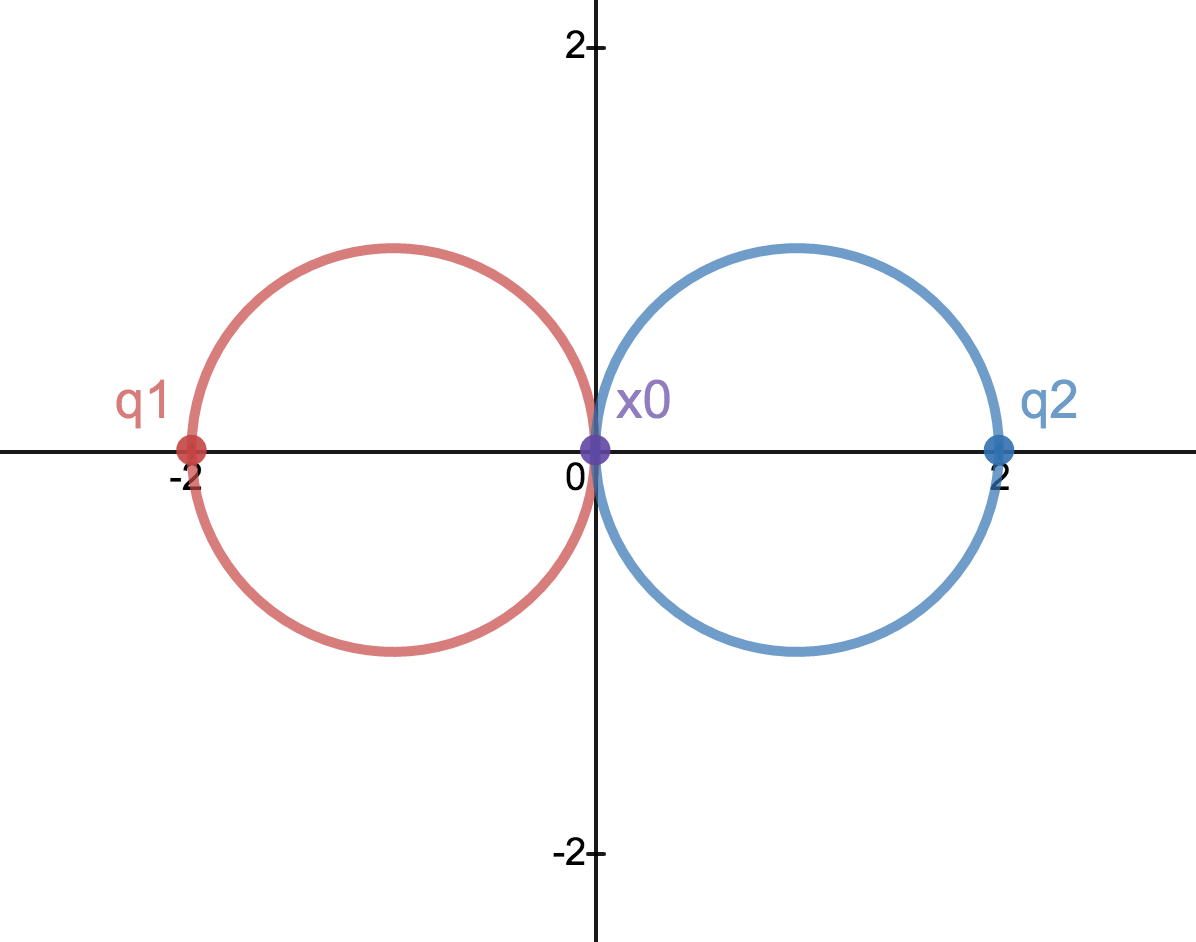
\includegraphics[width = 0.5\textwidth]{1.png}
        \caption{Plotted in \cite{Desmos}.}
        \label{fig:fig1}
    \end{figure}
    Then $X = U \cup V$ and $U$ and $V$ are both path-connected and open in $X$. Furthermore, $U \cap V = X \setminus \setb{ q_1 , q_2 }$ is path connected. Let $x_0 := (0,0) \in U \cap V$. Note that $W_i$ is homeomorphic to an open interval, so it is a deformation retract of $\setb{ x_0 }$. Thus $U$ and $V$ are homotopic to $S^1$ and $U \cap V$ is a deformation retract of $\setb{ x_0 }$, and so is simply connected. Thus $\pi_1(U,x_0) \cong \pi_1(V,x_0) \cong \z$. By a corollary of Seifert-van Kampen, 
    \[
        \pi_1(X,x_0) \cong \pi_1(U,x_0) \ast \pi_1(V,x_0) \cong \z \ast \z.
    \]
    Therefore $\pi_1(X,x_0)$, and hence the fundamental group of $S$, is infinite and nonabelian.
\end{proof}
\newpage
\section{Spring 1998 [Answered]}
Do \underline{seven} of the following 10 problems.
\subsection{Problem 1}
\begin{enumerate}[a)]
    \item State the ``least upper bound'' axiom for the real numbers.
    \item Suppose $f : [a,b] \to \real$ is continuous. Use the least upper bound property to show that $f \paren{ [a,b] }$ is bounded.
\end{enumerate}
\begin{proof}[Solution]
    \noindent
    \begin{enumerate}[a)]
        \item Every nonempty subset of $\real$ with an upper bound has a least upper bound.
        \item By Extreme Value Theorem, $f \paren{ [a,b] }$ is bounded.
    \end{enumerate}
\end{proof}
\subsection{Problem 2 \texorpdfstring{\cite{Munkres}}{}}
\begin{enumerate}[a)]
    \item Suppose $H$ is a connected subspace of a topological space and that $H \subseteq K \subseteq \overline{H}$. Show that $K$ is connected.
    \item Is it true if the word ``connected'' is replaced by ``path-connected'' everywhere? Either prove or give a counterexample.
\end{enumerate}
\begin{proof}[Solution]
    \noindent
    \begin{enumerate}[a)]
        \item We use the following result:
        \begin{lemma}
            Let $X$ be a topological space, and let $Y \subseteq X$. If $X$ has a separation $X = U \mid V$ and $Y$ is connected, then either $Y \subseteq U$ or $Y \subseteq V$.
        \end{lemma}
        \begin{proof}
            By way of contradiction, suppose otherwise. Then $U \cap Y$ and $V \cap Y$ are both nonempty and satisfy the following:
            \begin{enumerate}[(i)]
                \item $U \cap Y$ and $V \cap Y$ are both open in $Y$ by definition of the subspace topology.
                \item $\paren{U \cap Y} \cup \paren{V \cap Y} = \paren{U \cup V} \cap Y = X \cap Y = Y$.
                \item $\paren{U \cap Y} \cap \paren{V \cap Y} = \paren{U \cap V} \cap Y = \varnothing \cap Y = \varnothing$.
            \end{enumerate}
            Thus $U \cap Y$ and $V \cap Y$ form a separation of $Y$, which contradicts $Y$ being connected. Thus $Y$ must either lie entirely in $U$ or lie entirely in $V$.
        \end{proof}
        By way of contradiction, suppose that $K$ has a separation $K = U \mid V$. Since $H$ is connected, $H \subseteq U$ (without loss of generality) by the above lemma. By definition of separation, $U$ and $V$ are nonempty, and so there exists $y \in V$. Since $K \subseteq \overline{H}$, $y \in \overline{H}$ but $y \notin H$. Then $V$ is an open neighborhood of $y$ that does not intersect $H$, which is impossible since $y \in \overline{H}$. Thus no such $y$ exists and so $V$ is empty, a contradiction. Thus no such separation exists and so $K$ is connected.
        
        In particular, this implies that if $H$ is connected, then its closure $\overline{H}$ is also connected.
        \item False. Let 
        \[
            S := \setb{ \paren{ x , \sin \frac{1}{x} } \in \real^2 \, \middle| \, 0 < x \leq 1 }.
        \]
        $S$ is the image of of the connected set $(0,1]$ under the continuous map $(0,1] \to \real^2$, $x \mapsto \paren{ x , \sin \frac{1}{x} }$. Thus $S$ is connected, and its closure 
        \[
            \overline{S} = \paren{ \setb{ 0 } \times [0,1] } \cup S
        \]
        is also connected. Furthermore, since $S$ is the image of of the path-connected set $(0,1]$ under a continuous map, it is also path connected. However, we will show that $\overline{S}$ is \ita{not} path connected.
        
        By way of contradiction, suppose that $\overline{S}$ is path-connected. Let $p \in S$, then there exists a path $\gamma : [a,b] \to \overline{S}$ connecting the origin $(0,0)$ to $p$. Since $\setb{0} \times [0,1]$ is closed and $\gamma$ is continuous,
        \[
            \inv{\gamma} \paren{ \setb{0} \times [0,1] } \subset [0,1]
        \]
        is closed and so attains a maximum $c$. Thus $\gamma : [c,b] \to \overline{S}$ maps $c$ into the vertical interval $\setb{ 0 } \times [0,1]$ and maps $(c,b]$ into $S$. 
        
        Reparametrize $\gamma$ so that we can take $[c,b] = [0,1]$, and write $\gamma(t) = (x(t),y(t))$. Then $x(0) = 0$ while $x(t) > 0$ and $y(t) = \sin \paren{ \frac{1}{x(t)} }$ for $t > 0$. We show that there exists a sequence $t_n \to 0$ such that $y(t_n) = \paren{-1}^n$. Thus $y(t_n)$ does not converge, which contradicts the continuity of $\gamma$. Hence no such $\gamma$ exists and so $\overline{S}$ is not path-connected.
        
        For each $n \in \z^+$, choose $0 < u < x \paren{ \frac{1}{n} }$ such that $\sin \paren{ \frac{1}{n} } = (-1)^n$. By Intermediate Value Theorem, there exists $t_n$ with $0 < t_n < \frac{1}{n}$ such that $x(t_n) = u$.
    \end{enumerate}
\end{proof}
\subsection{Problem 3 \texorpdfstring{\cite{Munkres}}{}}
\begin{enumerate}[a)]
    \item Show that a closed subspace of a compact space is compact.
    \item Show that a compact subspace of a Hausdorff space is closed.
    \item Show that if $X$ is a compact Hausdorff topological space then no coarser or finer topology leaves $X$ both compact and Hausdorff.
\end{enumerate}
\begin{proof}[Solution]
    \noindent
    \begin{enumerate}[a)]
        \item Let $X$ be a compact space, and let $C \subseteq X$ be closed. Let $\mathcal{A}$ be an open cover of $C$. Then $\mathcal{U} := \mathcal{A} \cup \setb{ X \setminus C }$ is an open cover of $X$. Since $X$ is compact, there exists a finite subcover $\mathcal{U}' \subseteq \mathcal{U}$. Then $\mathcal{A}' :=  \mathcal{U}' \setminus \setb{ X \setminus C }$ is a finite subcover of $\mathcal{A}$, and so $C$ is compact.
        \item Let $X$ be a Hausdorff space, and let $K \subseteq X$ be compact. If $K = X$ then we are done, so suppose that $K \subsetneq X$. We show that $X \setminus K$ is open. Let $x_0 \in X \setminus K$. Since $X$ is Hausdorff, for each $x \in K$ there exists an open neighborhood $V_x$ and an open neighborhood $U_x$ of $x_0$ that are disjoint. Then the collection $\setb{ V_x }_{x \in K}$ is an open cover of $K$. Since $K$ is compact, there exists a finite subcover $\setb{ V_{x_i} }_{i = 1}^n$. Then 
        \[
            V := \bigcup\limits_{i = 1}^n V_{x_i}
        \]
        is an open set containing $K$, which is disjoint from 
        \[
            U := \bigcap\limits_{i = 1}^n U_{x_i}
        \]
        by construction. Since $x_0 \in U_{x_i}$ for all $1 \leq i \leq n$, $U$ is an open neighborhood of $x_0$ that is disjoint from $V$. Hence $U$ is also disjoint from $K$ and so $U \subseteq X \setminus K$. Therefore $X \setminus K$ is open and so $K$ is closed.
        \item See Fall 1997, Problem 4.
    \end{enumerate}
\end{proof}
\subsection{Problem 4 \texorpdfstring{\cite{Munkres}}{}}
Let $X$ and $Y$ be topological spaces.
\begin{enumerate}[a)]
    \item Define the product topology on $X \times Y$.
    \item If $X$ and $Y$ are compact, show that $X \times Y$ is compact.
\end{enumerate}
\begin{proof}[Solution]
    \noindent
    \begin{enumerate}[a)]
        \item Let $(X,\tau_X)$, $(Y,\tau_Y)$ be topological spaces. Then the product topology on $X \times Y$ is the topology generated by the base $\tau_X \times \tau_Y$.
        \item 
        \begin{lemma}[Tube Lemma]
            Let $X$, $Y$ be topological spaces, and suppose that $Y$ is compact. Let $x_0 \in X$, and suppose that $N \subseteq X \times Y$ is an open set containing $\setb{ x_0 } \times Y$. Then there exists an open neighborhood $W \subseteq X$ of $x_0$ such that $\setb{ x_0 } \times Y \subseteq W \times Y \subseteq N$.
        \end{lemma}
        \begin{proof}
            Let $\setb{ U_{\alpha} \times V_{\alpha} }_{\alpha \in J}$ be an open cover of $\setb{ x_0 } \times Y$, for $U_{\alpha} \subseteq X$ open and $V_{\alpha} \subseteq Y$ open such that $U_{\alpha} \times V_{\alpha} \subseteq N$ for all $\alpha \in J$. Since $\setb{ x_0 } \times Y \cong Y$ and $Y$ is compact, there exists a finite subcover $\setb{ U_i \times V_i }_{i = 1}^n$. If necessary, discard any element of this finite subcover that is disjoint from $\setb{ x_0 } \times Y$. Then as all of the $U_i \times V_i$'s intersect $\setb{ x_0 } \times Y$, $x_0 \in U_i$ for all $1 \leq i \leq n$. Define 
            \[
                W := \bigcup\limits_{i = 1}^n U_i.
            \]
            Then $W$ is an open neighborhood of $x_0$. Lastly, we show that $\setb{ U_i \times V_i }_{i = 1}^n$ covers $W \times Y$. Let $(x,y) \in W \times Y$, then $x \in U_i$ for all $1 \leq i \leq n$. Furthermore, as $\setb{ U_i \times V_i }_{i = 1}^n$ covers $\setb{ x_0 } \times Y$, $y$ will be contained in some $V_j$ for some $1 \leq j \leq n$. Thus $(x,y) \in U_j \times V_j$, and so \[
                W \times Y \subseteq \bigcup\limits_{i = 1}^n U_i \times V_i.
            \]
            Since $U_i \times V_i \subseteq N$ for all $1 \leq i \leq n$, $W \times Y \subseteq N$ as desired.
        \end{proof}
        Let $\mathcal{A}$ be an open cover of $X \times Y$, and let $x_0 \in X$. Since $\setb{ x_0 } \times Y \cong Y$, it is compact and so it is covered by finitely many elements $A_1 , \dotsc , A_m$ of $\mathcal{A}$. Then
        \[
            N := \bigcup\limits_{i = 1}^m A_i
        \]
        is an open set containing $\setb{ x_0 } \times Y$. By the Tube Lemma, there exists $W \subseteq X$ open such that $\setb{ x_0 } \times Y \subseteq W \times Y \subseteq N$. Thus $W \times Y$ is also covered by $A_1 , \dotsc , A_m$.
        
        Thus for each $x \in X$, there exists a neighborhood $W_x$ of $x$ such that $W_x \times Y$ is covered by finitely many elements of $\mathcal{A}$. Then the collection of all such $W_x$ is an open cover of $X$. By compactness of $X$ there exists a finite subcover $W_1 , \dotsc , W_n$ that covers $X$. Then the collection of tubes $W_1 \times Y , \dotsc , W_n \times Y$ covers $X \times Y$. Since each tube is covered by finitely many elements of $\mathcal{A}$, $X \times Y$ is also covered by finitely many elements of $\mathcal{A}$. Therefore $X \times Y$ is compact.
    \end{enumerate}
\end{proof}
\subsection{Problem 5 \texorpdfstring{\cite{Munkres}}{}}
Suppose $X$ and $Y$ are Hausdorff spaces and $f : X \to Y$ is continuous. Let the \underline{graph} of $f$ in $X \times Y$ be the set $G_f := \setb{ (x,y) \mid y = f(x) }$.
\begin{enumerate}[a)]
    \item Show that $G_f$ is a closed subspace of $X \times Y$.
    \item What if $Y$ is Hausdorff and $X$ is not?
\end{enumerate}
\begin{proof}[Solution]
    \noindent
    \begin{enumerate}[a)]
        \item We show that $( X \times Y ) \setminus G_f$ is open: let $(x,y) \in ( X \times Y ) \setminus G_f$. Then $y \neq f(x)$, and since $Y$ is Hausdorff there exists disjoint open neighborhoods $V_1$, $V_2$ of $y$ and $f(x)$, respectively. Since $f$ is continuous, $U := \inv{f}(V_2)$ is open in $X$ and $x \in \inv{f}(V_2)$. Thus $U \times V_1$ is an open neighborhood of $(x,y)$ in $X \times Y$. We claim that $U \times V_1$ is disjoint from $G_f$: let $(a,b) \in U \times V_1$. Then $a \in U = \inv{f}(V_2)$ and so $f(a) \in V_2$. Since $V_2 \cap V_1 = \varnothing$, $f(a) \neq b$, and so $(a,b) \notin G_f$. Thus $(U \times V_1) \cap G_f = \varnothing$, and so $U \times V_1$ is an open neighborhood of $(x,y)$ that is contained in $( X \times Y ) \setminus G_f$. Thus $( X \times Y ) \setminus G_f$ is open.
        \item Note that the solution to a) did not require $X$ to be Hausdorff at all. Thus $G_f$ is still closed in $X \times Y$ even if $X$ is not Hausdorff. 
    \end{enumerate}
\end{proof}
\subsection{Problem 6 \texorpdfstring{\cite{stm}}{}}
Suppose $(M,d)$ is a metric space.
\begin{enumerate}[a)]
    \item Show that $d : M \times M \to \real_{\geq 0}$ is continuous. 
    \item State what the intermediate value property says about a continuous function $f : [a,b] \to \real$.
    \item Suppose $f : [0,1] \to M$ is a continuous function and $f(0) \neq f(1)$. Show that $M$ has uncountably many points.
\end{enumerate}
\begin{proof}[Solution]
    \noindent
    \begin{enumerate}[a)]
        \item For lack of confusion, denote an open interval $(a,b) \subseteq \real$ by $]a,b[$ (similarly for half-open half-closed intervals). 
        
        Let $U \subseteq \mathbb{R}_{\geq 0}$ be open. Without loss of generality, take $U$ to either be $]a,b[$ or $[0,b[$ for some $0 \leq a < b \leq \infty$.
        \begin{enumerate}[(i)]
            \item Case 1: $U = ]a,b[$. Let $(x_0,y_0) \in \inv{d}(U)$. Then $a < d(x_0,y_0) < b$. Let $r > 0$, then $B_{r}(x_0) \times B_{r}(y_0)$ is an open neighborhood of $(x_0,y_0)$ in $M^2$. For all $(x,y) \in B_r(x_0) \times B_r(y_0)$,
            \begin{align*}
                d(x,y) & \leq d(x,x_0) + d(x_0,y) \\
                & < r + d(x_0,y_0) + d(y_0,y) \\
                & < 2r + d(x_0,y_0),
            \end{align*}
            and 
            \begin{align*}
                d(x_0,y_0) & \leq d(x_0,y) + d(y,y_0) \\
                & < d(x_0,x,) + d(x,y) + r \\
                & < 2r + d(x,y).
            \end{align*}
            Since $a < d(x_0,y_0) < b$, we can choose $r$ small enough such that $]d(x_0,y_0) - 2r , d(x_0,y_0) + 2r[ \subseteq ]a,b[$ (choose $2r \leq \min \setb{ b - d(x_0,y_0) , d(x_0,y_0) - a }$). Then
            \begin{align*}
                d(x,y) & < 2r + d(x_0,y_0) < b, \\
                d(x,y) & > d(x_0,y_0) - 2r > a.
            \end{align*}
            Thus $a < d(x,y) < b$ and so $d(x,y) \in \inv{d}(U)$.
            \item Case 2: $U = [0,b)$. Using a similar strategy as Case 1, we can find an open neighborhood $B_r(x_0) \times B_r(y_0)$ of $(x_0,y_0)$ such that $B_r(x_0) \times B_r(y_0) \subseteq \inv{d}(U)$.
        \end{enumerate}
        In both cases, $\inv{d}(U)$ is open, and so $d$ is continuous. Furthermore, $d$ is continuous in both variables separately.
        \item Let $f : [a,b] \to \real$ be continuous, and suppose that $f(a) \neq f(b)$. Let $c := \min \setb{ f(a) , f(b) }$, $d := \max \setb{ f(a) , f(b) }$. By the intermediate value property, 
        \[
            [c,d] \subseteq f \paren{ [a,b] }.
        \]
        \item Let $f : [0,1] \to M$ be continuous with $f(0) \neq f(1)$. Let $g : M \to \real$ be given by $g(x) := d(f(0),x)$. By part (a), $g$ is continuous, and so the composition $h := g \circ f : [0,1] \to \real$ is continuous. Since $f(0) \neq f(1)$, $h(0) = 0$ and $r := h(1) > 0$. By the Intermediate Value Theorem, 
        \[
            [0,r] \subseteq h \big( [0,1] \big) = g \Big( f \big( [0,1] \big) \Big).
        \]
        Since $[0,r]$ is uncountable, so is $g \Big( f \big( [0,1] \big) \Big)$. Thus the cardinality of $f \big( [0,1] \big)$ is at least the cardinality of $g \Big( f \big( [0,1] \big) \Big)$, and so $f \big( [0,1] \big)$ is uncountable. Since $f \big( [0,1] \big) \subseteq M$, $M$ is uncountable.
    \end{enumerate}
\end{proof}
\subsection{Problem 7 \texorpdfstring{\cite{Munkres,Jacob}}{}}
Suppose $X$ is a Hausdorff space, $q : X \to Y$ is a surjection, and the set $Y$ is given the quotient topology. Further suppose that, with these topologies, $q$ is a closed map and for each $y \in Y$, $\inv{q}(y)$ is compact. Prove that $Y$ is Hausdorff.
\begin{proof}[Solution]
    \begin{lemma}
        Let $X$ be a Hausdorff space, and let $A , B \subseteq X$ be disjoint and compact. Then there exists disjoint open subsets $U , V \subseteq X$ such that $A \subseteq U$ and $B \subseteq V$.
    \end{lemma}
    \begin{proof}
        First, we show that for any compact subspace $K \subseteq X$ and $x_0 \notin K$, there exists disjoint open subsets $U , V \subseteq X$ such that $x_0 \in U$ and $K \subseteq V$. For each $y \in K$, there exists disjoint open neighborhoods $U_y$ and $V_y$ of $x_0$ and $y$, respectively. Then the collection of all such $V_y$'s covers $K$. By compactness of $K$ there exists a finite subcover $V_1 , \dotsc , V_n$. Let 
        \[
            V := \bigcup\limits_{i = 1}^n V_i,
        \]
        and let
        \[
            U := \bigcap\limits_{i = 1}^n U_i,
        \]
        where $U_i$ is the corresponding open set to $V_i$. Then $U$ is an open neighborhood of $x_0$ and $K \subseteq V$, and $U \cap V = \varnothing$: for any $z \in V$, $z \in V_i$ for some $1 \leq i \leq n$. Then $z \notin U_i$, so $z \notin U$. 
        
        Now, we prove the lemma. Fix $x \in A$. Since $A$ and $B$ are disjoint, there exists an open neighborhood $U_x$ of $x$ and an open set $V_x$ containing $B$ such that $U_x \cap V_x = \varnothing$. Then the collection of all such $U_x$ is an open cover of $A$, so by compactness of $A$ there exists a finite subcover $U_1 , \dotsc , U_n$. Let
        \[
            U := \bigcup\limits_{i = 1}^n U_i,
        \]
        and let
        \[
            V := \bigcap\limits_{i = 1}^n V_i,
        \]
        where $V_i$ is the corresponding open set to $U_i$. Then $U$ and $V$ are open sets that contain $A$ and $B$, respectively, and are disjoint: for any $z \in U$, $z \in U_i$ and so $z \notin V_i$. Hence $z \notin V$. 
    \end{proof}
    By uniqueness of the quotient topology on $Y$, $q : X \to Y$ is the quotient map, and so $q$ is also continuous. 
    
    Let $y_1 , y_2 \in Y$ be distinct. Then for each $i = 1, 2$, $K_i := \inv{q} \paren{ \setb{ y_i } } \subseteq X$ is compact. Furthermore $K_1$ and $K_2$ are disjoint. Since $X$ is Hausdorff, there exists two disjoint open subsets $U , V \subset X$ such that $K_1 \subseteq U$ and $K_2 \subseteq V$. By the lemma, there exists disjoint open sets $U , V \subset X$ such that $K_1 \subseteq U$ and $K_2 \subseteq V$. Then $X \setminus U$ is a closed set containing $K_2$ but not $K_1$, and $X \setminus V$ is a closed set containing $K_1$ but not $K_2$. Since $q$ is a closed map, $q(X \setminus U)$ is closed in $Y$ and contains $y_2$ but not $y_1$, and $q(X \setminus V)$ is closed in $Y$ and contains $y_1$ but not $y_2$. Then $Y \setminus q(X \setminus U)$ is an open neighborhood of $y_1$ and $Y \setminus q(X \setminus V)$ is an open neighborhood of $y_2$. Lastly,
    \begin{align*}
        \big( Y \setminus q(X \setminus U) \big) \cap \big( Y \setminus q(X \setminus V) \big) & = Y \setminus \big( q(X \setminus U) \cup q(X \setminus V) \big) \\
        & = Y \setminus \Big( q \big( ( X \setminus U ) \cup (X \setminus V) \big) \Big) \\
        & = Y \setminus \Big( q \big( X \setminus ( \underbrace{ U \cap V }_{ = \varnothing } ) \big) \Big) \\
        & = Y \setminus \big( q(X \setminus \varnothing) \big) \\
        & = Y \setminus \big( q(X) \big) \\
        & = Y \setminus Y \\
        & = \varnothing.
    \end{align*}
    Therefore $Y$ is Hausdorff.
\end{proof}
\subsection{Problem 8}
\begin{enumerate}[a)]
    \item Suppose $X$ is a simply connected locally path connected space. Show that any map $f : X \to S^1 \times S^1 \times S^1$ is null-homotopic.
    \item Is a) true if $S^1 \times S^1 \times S^1$ is replaced by the projective plane $\mathbb{RP}^2$? Either prove it or exhibit a counterexample and prove it is one.
\end{enumerate}
\begin{proof}[Solution]
    UNFINISHED
    \begin{enumerate}[a)]
        \item 
        \item 
    \end{enumerate}
\end{proof}
\subsection{Problem 9 \texorpdfstring{\cite{Ricky}}{}}
Show that $\real^2$ and $\real^n$, $n \neq 2$, are not homeomorphic. (Hint: You may take as given that $\pi_1(S^1) = \z$.)
\begin{proof}[Solution]
    First, we show that $\real \not\cong \real^2$. Note that if $f : X \to Y$ is a homeomorphism, then the restriction of $f : \setminus \setb{ x_0 } \to Y \setminus \setb{ f(x_0) }$ for some $x_0 \in X$ is still a homeomorphism. By way of contradiction, suppose that there exists a homeomorphism $f : \real^2 \to \real$. Then the restriction of $f : \real \setminus \setb{ (0,0) } \to \real \setminus \setb{ f(0,0) }$ is also a homeomorphism. Note that $\real^2 \setminus \setb{ f(0) }$ is connected since it is path connected. Note that $\real \setminus \setb{ f(0,0) }$ is not connected, having separation $(-\infty, f(0,0)) | (f(0,0) , \infty)$. Since connectedness is a topological property, $f \paren{ \real^2 \setminus \setb{ (0,0) } } = \real \setminus \setb{ f(0,0) }$ is connected. But this contradicts $\real \setminus \setb{ f(0,0) }$ being not connnected. Hence no such homeomorphism $f : \real^2 \to \real$ exists, and so $\real$ and $\real^2$ are not homeomorphic. 
    
    Next, we show that $\real^2 \not\cong \real^n$ for $n > 2$. Note that for $n \geq 2$, $S^{n-1}$ is a deformation retract of $\real^n \setminus \setb{ \mathbf{0} }$, and so the two spaces are homotopy equivalent. Since $S^{n-1}$ is simply connected for $n > 2$, $\real^n \setb{ \mathbf{0} }$ is also simply connected for $n > 2$. However, since $\pi_1(S^1) \cong \z$, $S^1$ is not simply connected and so $\real^2 \setminus \setb{ (0,0) }$ is not simply connected. Thus $\real^2 \setminus \setb{ (0,0) }$ and $\real^n \setb{ \mathbf{0} }$ are not homeomorphic for $n > 2$. By similar reasoning as above, $\real^2$ and $\real^n$ are not homeomorphic for $n > 2$. 
\end{proof}
\subsection{Problem 10}
Show that there is no retraction of the M\"obius band onto its boundary.
\begin{proof}[Solution]
    UNFINISHED
\end{proof}
\newpage
\section{Fall 1998}
Answer six questions.
\subsection{Problem 1 \texorpdfstring{\cite{DF,Rico}}{}}
Let $G$ be a group and let $\mathcal{F}$ be the set of all cosets of the form $g \cdot H$, where $H$ runs over all normal subgroups of finite index in $G$ and $g$ runs over all elements of $G$.
\begin{enumerate}[(i)]
    \item Show that $\mathcal{F}$ is a basis of open sets for a topology on $G$.
    \item Show that group multiplication and the map $x \to \inv{x}$ are continuous in this topology.
    \item State and prove a group theoretic condition on $G$ which is equivalent to this topology being Hausdorff.
    \item Show that every set $\mathcal{F}$ is \textbf{closed} in this topology.
    \item By considering the case that $G$ is the integers or otherwise, prove that the integers contain infinitely many primes.
\end{enumerate}
\begin{proof}[Answer]
    \noindent
    \begin{enumerate}[(i)]
        \item Let $e$ denote the identity element of $G$. Since $G$ is a normal subgroup of itself with finite index ($[G:G] = 1$), $G = eG \in \mathcal{F}$ and so every element of $G$ is contained in an element of $\mathcal{F}$. Next, let $g \in G$ and suppose that $g \in B_1 \cap B_2$ for  $B_i \in \mathcal{F}$, $i = 1,2$. Then $B_i = g_i H_i$ for some $g_i \in G$ and $H_i \trianglelefteq G$ with finite index. Then $g = g_1 h_1 = g_2 h_2$ for some $h_i \in H_i$. Then $g \inv{g_i} = h_i$, and so $gH = g_i H_i$. Thus $g_1 H_1 \cap g_2 H_2 = g H_1 \cap g H_2$. 
        \begin{claim}
            $g H_1 \cap g H_2 = g \paren{ H_1 \cap H_2 }$. 
        \end{claim}
        \begin{proof}
            Let $k \in g H_1 \cap g H_2$, then $k = g h_i$ for some $h_i \in H_i$. Then $g h_1 = g h_2$, and so $h_1 = h_2 =: h$. Thus $h \in H_1 \cap H_2$, and so $k = g h \in g \paren{ H_1 \cap H_2 }$. Conversely, let $k \in g \paren{ H_1 \cap H_2 }$, then $k = g h$ for some $h \in H_1 \cap H_2$. Thus $k \in g H_1$ and $k \in g H_2$, hence $k \in g H_1 \cap g H_2$. 
        \end{proof}
        \begin{claim}
            $H_1 \cap H_2$ is a normal subgroup of $G$.
        \end{claim}
        \begin{proof}
            Let $g \in G$, $h \in H_1 \cap H_2$. Then as $h \in H_1$ and $H_1$ is normal, $g h \inv{g} \in H_1$. Similarly, $g h \inv{g} \in H_2$. Therefore $H_1 \cap H_2 \trianglelefteq G$.
        \end{proof}
        \begin{claim}
            $H_1 \cap H_2$ has finite index in $G$.
        \end{claim}
        \begin{proof}
            Recall that if $H \leq K \leq G$, then 
            \[
                \sqbrack{ G : H } = \sqbrack{ G : K } \sqbrack{ K : H },
            \]
            where if one side of the equality is infinite, so is the other. Then 
            \[
                \sqbrack{ G : H_1 \cap H_2 } = \sqbrack{ G : H_1 } \sqbrack{ H_1 : H_1 \cap H_2 } = \sqbrack{ G : H_2 } \sqbrack{ H_2 : H_1 \cap H_2 }.
            \]
            Since $H_1$ has finite index, it suffices to show that $H_1 \cap H_2$ has finite index in $H_1$. Now, recall Second Isomorphism Theorem: if $A , B \leq G$ such that $A \leq N_G(B)$, then $AB \leq G$, $B \trianglelefteq AB$, $A \cap B \trianglelefteq A$, and $AB / B \cong A / \paren{ A \cap B }$. Applying this to $H_1$ and $H_2$ gives us 
            \[
                H_1 H_2 / H_2 \cong H_1 / \paren{ H_1 \cap H_2 },
            \]
            and so 
            \[
                \sqbrack{ H_1 H_2 : H_2 } = \sqbrack{ H_1 : H_1 \cap H_2 }.
            \]
            Since $\sqbrack{ H_1 H_2 : H_2 }$ is the number of (left) cosets of $H_2$ in $H_1 H_2$, and since $H_1 H_2 \leq G$, $\sqbrack{ H_1 H_2 : H_2 } \leq \sqbrack{ G : H_2 } < \infty$. Thus $\sqbrack{ H_1 : H_1 \cap H_2 }$ is finite.
        \end{proof}
        Therefore $B_1 \cap B_2$ is itself an element of $\mathcal{F}$, and so $\mathcal{F}$ is a basis for a topology on $G$.
        \item Let $f : G \times G \to G$, $f(g,h) := gh$. It suffices to show that the preimage of a basis element is open, then as any open set $U \subseteq G$ is the union of basis elements, we have
        \[
            \inv{f}(U) = \inv{f} \paren{ \bigcup\limits_{ \alpha \in J} B_{\alpha} } = \bigcup\limits_{ \alpha \in J } \inv{f} \paren{ B_{\alpha} }, 
        \]
        and so $\inv{f}(U)$ is open. Let $B \in \mathcal{F}$, then $B = xH$ for some $x \in G$, $H \trianglelefteq G$ of finite index. Then 
        \[
            \inv{f} (xH) = \setb{ \paren{ g_1 , g_2 } \in G \times G \, \middle| \, g_1g_2 \in gH }.
        \]
        Then for $\paren{ g_1 , g_2 } \in \inv{f}(xH)$, $g_1 g_2 = x h$ for some $h \in H$. Thus $g_2 = \inv{g_1} g h$, and so we can write $\paren{ g_1 , g_2 } = \paren{ g_1 , \inv{g_1} xh }$, and so 
        \[
            \inv{f}(xH) = \setb{ \paren{ g_1 , \inv{g_1} gh } \in G \times G \, \middle| \, g_1 \in G , h \in H } = G \times \paren{ \bigcup\limits_{g \in G} \inv{g} x H }  ,
        \]
        which is open in $G \times G$ with the product topology, since $G , \paren{ \inv{g} x } H \in \mathcal{F}$ for each $g \in G$. Thus $f$ is continuous.
        
        Now, let $\varphi : G \to G$, $\varphi(g) := \inv{g}$. Note that $\varphi$ is a bijection. Again, it suffices to show that $\inv{\varphi}(B)$ is open in $G$ for $B \in \mathcal{F}$. Let $B = xH \in \mathcal{F}$, then if $g \in \inv{\varphi}(xH)$, $\varphi(g) = \inv{g} = xH$, so $\inv{g} = xh$ for some $h \in H$. Thus $g = \inv{xh} = \inv{h} \inv{x}$, and so \[
            \inv{\varphi}(xH) = \setb{ \inv{h} \inv{x} \, \middle| \, h \in H } = H \inv{x}.
        \]
        Since $H$ is a normal subgroup of $G$, $H \inv{x} = \inv{x} H$ and so $\inv{\varphi}(xH)$ is a basis element, and thus is open. Therefore $\varphi$ is continuous.
        
        Note that this makes $\varphi$ a homeomorphism from $G$ to itself. However, $\varphi$ is an \ita{isomorphism} if and only if $G$ is abelian.
        \item Note that if $(X,\tau)$ is a topological space with base $\mathcal{B}$, then it suffices to use basis elements to show that $(X,\tau)$ is Hausdorff. [UNFINISHED]
        \item Since basis elements are themselves open, this shows that if $G$ has more than one element, then $G$ is not connected with this topology. 
        \item 
    \end{enumerate}
\end{proof}
\subsection{Problem 2 \texorpdfstring{\cite{Leon,proper}}{}}
For each of the following, say whether it is true or false. Give a proof or counterexample as appropriate.
\begin{enumerate}[(i)]
    \item $[0,1) \times [0,1)$ is homeomorphic to $[0,1) \times [0,1]$.
    \item A function between Hausdorff topological spaces is continuous if the preimage of every compact set is compact.
    \item If a function between Hausdorff topological spaces is continuous, then the preimage of every compact set is compact.
    \item A compact topological space is metrizable.
    \item If $A$ is a path connected subset of a compact metric space $X$, then the closure of $A$ in $X$ is also path-connected.
\end{enumerate}
\begin{proof}[Answer]
    \noindent
    \begin{enumerate}[(i)]
        \item True, both are homeomorphic to a half-open disk.
        \item False. Note that a map satisfying such a property is called a proper map. Let $X := [0,1]$, $Y := \real$, $f : X \to Y$ given by 
        \[
            f(x) := 
            \begin{cases}
                \frac{1}{x} , & \quad 0 < x \leq 1, \\
                0 , & \quad x = 0.
            \end{cases}
        \]
        Since $[0,1]$ and $\real$ are metric spaces, they are Hausdorff. Clearly $f$ is not continuous, however we show that $f$ is a proper map. Let $K \subset \real$ be compact. Since $[0,1]$ is bounded $\inv{f}(K) \subseteq [0,1]$ is also bounded, so by Heine-Borel it suffices to show that $\inv{f}(K)$ is closed. Note that $\inv{f}(K)$ is the preimage of $K$ under the restriction of $f$ to $(0,1]$ unioned with $\setb{ 0 }$ if $0 \in K$. Since the restriction of $f$ to $(0,1]$ \ita{is} continuous and $K$ is closed, the preimage of $K$ under the restriction of $f$ is closed. Regardless of whether $0 \in K$, then $\inv{f}(K)$ is closed since it is the union of finitely many open sets. Hence $\inv{f}(K)$ is closed in $[0,1]$ and hence compact. 
        \item False. Let $X := Y := \real$, $f : X \to Y$ be given by $f(x) := \sin x$. Clearly $\real$ is Hausdorff, $f$ is continuous, and $K := [-1,1] \subset \real$ is compact. However, the preimage of $K$ uner $f$ is all of $\real$, which is not compact.
        \item False. Recall that every finite topological space is compact, and that every metric space is Hausdorff. Then the set $X := \setb{0,1}$ with the indiscrete topology $\tau = \setb{ \varnothing , X }$ is a finite topological space, and thus compact. However, $X$ is clearly not Hausdorff, as the only neighborhood of $0$ and $1$ is $X$ itself, and so $0$ and $1$ have no disjoint open neighborhoods. Thus $X$ is not metrizable.
        \item False. Take the answer to Fall 1997, Problem 2. Treat $S \subset X := [0,1] \times [-1,1]$. $X$ is compact, and since it is a subspace of $\real^2$ it is metrizable. $S$ is path connected, but the closure of $S$ in $X$ is not.
    \end{enumerate}
\end{proof}
\subsection{Problem 3 \texorpdfstring{\cite{Munkres,Blair}}{}}
Give a careful definition of \ita{connected}.
\begin{enumerate}[(i)]
    \item Prove that the closed interval $[0,1]$ (with the usual topology) is connected.
    \item Show that a connected metric space with at least two points is uncountable.
\end{enumerate}
\begin{proof}[Answer]
    A topological space $X$ has a \underline{separation} $X = U \mid V$ if there exists two disjoint nonempty open subsets $U , V \subset X$ such that $X = U \cup V$. $X$ is \textbf{connected} if it has no separation.
    \begin{enumerate}[(i)]
        \item By way of contradiction, suppose that $[0,1]$ has a separation $[0,1] = U \mid V$. Pick $a \in U$, $b \in V$. Then $a \neq b$ and without loss of generality, take $a < b$. Let $U_0 := [a,b] \cap U$, and let $V_0 := [a,b] \cap V$. We claim that $[a,b]$ has separation $[a,b] = U_0 \mid V_0$. 
        \begin{itemize}
            \item Since $a \in U_0$, $U_0 \neq \varnothing$, and since $b \in V_0$, $V_0 \neq \varnothing$.
            \item $U_0$ and $V_0$ are both open in the subspace topology of $[a,b]$.
            \item Note that 
            \begin{align*}
                U_0 \cap V_0 & = \paren{ [a,b] \cap U } \cap \paren{ [a,b] \cap V } \\
                & = [a,b] \cap \paren{ U \cap V } \\
                & = [a,b] \cap \varnothing \\
                & = \varnothing.
            \end{align*}
            \item Lastly,
            \begin{align*}
                [a,b] & = [a,b] \cap [0,1] \\
                & = [a,b] \cap \paren{ U \cup V } \\
                & = \paren{ [a,b] \cap U } \cup \paren{ [a,b] \cap V } \\
                & = U_0 \cup V_0.
            \end{align*}
        \end{itemize}
        Thus $[a,b]$ has a separation $[a,b] = U_0 \mid V_0$.
        
        Since $U_0$ is bounded, it has a supremum $c := \sup U_0$. We have two cases to consider:
        \begin{itemize}
            \item Case 1: $c \in U_0$. Then $c \neq b$ (since $b \in V_0$), so either $c = a$ or $c > a$. If $c = a$, then $U_0$ is open in $[a,b]$ there exists $\epsilon > 0$ such that $[a,a+\epsilon) \subseteq U_0$. Then there exists $u \in U_0$ such that $a < u < a + \epsilon$, which contradicts $a = c$ being an upper bound for $U_0$. Thus $c > a$. Thus there exists $\epsilon > 0$ such that $(c - \epsilon , c + \epsilon) \cap [a,b] \subseteq U_0$. Then there exists $u \in U_0$ such that $c < u < c + \epsilon$, which contradicts $c$ being an upper bound of $U_0$. Thus $c \notin U_0$ and so $c \in V_0$.
            \item Case 2: $c \in V_0$. Then $c \neq a$ (since $a \in U_0$). Thus either $c = b$ or $c < b$. If $c = b$, then there exists $\epsilon > 0$ such that $(b-\epsilon,b] \subseteq V_0$. Since $U_0$ and $V_0$ are disjoint, $b - \frac{\epsilon}{2} < b$ is not contained in $U_0$, and so $b - \frac{\epsilon}{2}$ must be greater than every element of $U_0$ (else a contradiction to either $(b-\epsilon,b] \subseteq V_0$ or $c = \sup U_0$). But then $b - \frac{\epsilon}{2}$ is a smaller upper bound for $U_0$ than $b = c$, which is impossible, hence $c < b$. Again, there exists $\epsilon > 0$ such that $(c-\epsilon , c+\epsilon) \cap [a,b] \subseteq V_0$. Then there exists $v \in V_0$ such that $c - \epsilon < v < c - \frac{\epsilon}{2}$, and so $c - \frac{\epsilon}{2} > u$ for all $u \in U_0$. Thus $c - \frac{\epsilon}{2} > c$, which is absurd. Thus $c \notin V_0$.
        \end{itemize}
        Thus $c \notin U_0$ and $c \notin V_0$, and so $c \notin [a,b]$, which is absurd. Therefore no such separation of $[0,1]$ exists and so $[0,1]$ is connected.
        \item See Spring 1998, Problem 6c).
    \end{enumerate}
\end{proof}
\subsection{Problem 4 \texorpdfstring{\cite{Munkres}}{}}
\begin{enumerate}[(i)]
    \item Let $(X,d)$ be a compact metric space and let $f : X \to X$ be a map with the property that 
    \[
        d \paren{ f(x) , f(y) } < d(x,y)
    \]
    for every distinct $x , y \in X$.
    
    Prove that there is a unique point $x_0$ with $f(x_0) = x_0$.
    \item Let $(X,d)$ be a compact metric space and let $f : X \to X$ be a continuous map with the property that for every $\epsilon > 0$, there is an $x_{\epsilon}$ so that $d \paren{ x_{\epsilon} , f(x_{\epsilon}) } < \epsilon$. Prove that $f$ has a fixed point. Need this fixed point be unique?
\end{enumerate}
\begin{proof}[Answer]
    \noindent
    \begin{enumerate}[(i)]
        \item 
        \begin{lemma}
            Let $(X,d)$ be a metric space, $A \subseteq X$ nonempty. Let 
            \[
                \delta A := \sup \setb{ d(x,y) \mid x , y \in A }
            \]
            be the diameter of $A$. Then $\delta A = 0$ if and only if $A$ consists of one element.
        \end{lemma}
        \begin{proof}
            Clearly if $A = \setb{ a }$, then $d(x,y) = 0$ for all $x , y \in A$, and so $\delta A = 0$. Conversely, suppose that $\delta A = 0$. Then $d(x,y) \leq 0$ for all $x , y \in A$. By properties of the metric, $x = y$ for all $x , y \in A$, and so $A$ only has one element.
        \end{proof}
        \begin{remark}
            The diameter of the empty set is not defined in general. Some sources take it to be zero, others $-\infty$, and others do not define it for the empty set at all.
        \end{remark}
        Such a map is called a \textbf{shrinking map}. Note that $f$ is continuous, in fact uniformly so, since for any $\epsilon > 0$ and $x , y \in X$ with $d(x,y) < \epsilon$, $d \paren{ f(x) , f(y) } < \epsilon$.
        
        For each $n \in \z^+$, let $f^1 := f$ and $f^n := f \circ f^{n-1}$. Let $A_n := f^n(X)$, and let
        \[
            A := \bigcap\limits_{n = 1}^{\infty} A_n.
        \]
        Since $f$ is continuous, $A_n$ is compact (and nonempty) for all $n \in \z^+$. Since $X$ is compact and $A_{n+1} \subseteq A_n$ for all $n \in \z^+$, $A$ is nonempty by the finite intersection property. Let $x \in A$, and for each $n \in \z^+$ choose $x_n$ such that $x = f^{n+1} \paren{ x_{n} }$. By compactness of $X$, sequence $\setb{ y_n := f^n \paren{ x_n } }_{n = 1}^{\infty} \subseteq X$ has a convergent subsequence with limit, say, $a \in X$. 
        \begin{claim}
            $a \in A$.
        \end{claim}
        \begin{proof}
            It suffices to show that $a \in A_n$ for all $n \in \z^+$. UNFINISHED
        \end{proof}
        \begin{claim}
            $f(a) = x$.
        \end{claim}
        \begin{proof}
            By choice of $x_n$, 
            \begin{align*}
                x & = f^{n+1} \paren{ x_{n} } \\
                & = f \paren{ f^{n} \paren{ x_n } } \\
                & = f \paren{ y_n }
            \end{align*}
            for all $n \in \z^+$, and so by continuity of $f$,
            \begin{align*}
                \lim\limits_{k \to \infty} x & = \lim\limits_{k \to \infty} f \paren{ y_{n_k} } \\
                x & = f \paren{ \lim\limits_{k \to \infty} y_{n_k} } \\
                & = f(a).
            \end{align*}
        \end{proof}
        Since $x \in A$ was arbitrary, $A = f(A)$. UNFINISHED
        \item UNFINISHED
    \end{enumerate}
\end{proof}
\subsection{Problem 5 \texorpdfstring{\cite{Berge}}{}}
Define a \ita{contraction mapping} of a metric space.
\begin{enumerate}[(i)]
    \item Show that a contraction mapping of a complete metric space has a fixed point and that this fixed point is unique.
    \item Let $E$ be the set of continuous functions from $[0,1]$ to itself with metric $d(f,g) = \sup\limits_{0 \leq x \leq 1} |f(x) - g(x)|$.
    
    Prove that the map $A : E \to E$ given by $(Af)(x) = 1 - \frac{1}{3}x^3f(1-x)$ is a contraction.
    \item Prove that if $h_*$ is the fixed function of the map $A$ and if $h_0$ is the function which is identically 1, then 
    \[
        d(A^nh_0,h_*) \leq \frac{1}{3^{n+1}}.
    \]
\end{enumerate}
\begin{proof}[Answer]
    A \textbf{contraction mapping} of a metric space $(X,d)$ is a function $f : X \to X$ such that for all $x, y \in X$,
    \[
        d \paren{ f(x) , f(y) } \leq C d(x,y)
    \]
    for some $0 < C < 1$. 
    \begin{enumerate}[(i)]
        \item Let $f : X \to X$ be a contraction mapping, then for all $x, y \in X$,
        \[
            d \paren{ f(x) , f(y) } \leq C d(x,y)
        \]
        for some $0 < C < 1$. Note that a contraction mapping is continuous (in fact uniformly so), since for any $\epsilon > 0 $,
        \[
            d \paren{ f(x) , f(y) } \leq C d(x,y) < \epsilon
        \]
        if $d(x,y) < \frac{\epsilon}{C}$.
        
        Fix $x_0 \in X$, and for each $n \in \z^+$ let $x_n := f^{n}(x_0)$. Then 
        \begin{align*}
            d \paren{x_n,x_{n+1}} & = d \paren{ f^n(x_0) , f^{n+1}(x_0) } \\
            & < C d \paren{ x_{n-1} , x_n } \\
            & < \cdots \\
            & < C^n d \paren{ x_0 , f(x_0) }.
        \end{align*}
        Then for any $p > 0$, 
        \[
            d \paren{ x_n , x_{n+p} } \leq d(x_0,f(x_0)) \sum\limits_{k = n}^{n+p} C^k.
        \]
        Since $0 < C < 1$, for any $\epsilon > 0$ there exists $N$ such that for all $m > n > N$, 
        \[
            d \paren{ x_n , x_m } \leq d(x_0,f(x_0)) \sum\limits_{k = n}^{m} C^k < \epsilon.
        \]
        Thus $\setb{ x_n }_{n=1}^{\infty}$ is a Cauchy sequence, and by completeness of $(X,d)$, it has a limit $x_* \in X$. Hence by continuity of $f$, 
        \begin{align*}
            \lim\limits_{n\to\infty} x_{n+1} & = \lim\limits_{n \to \infty} f(x_n) \\
            x_* & = f(x_*)
        \end{align*}
        and so $x_*$ is a fixed point of $f$. For uniqueness, suppose that $y_* \in X$ is another fixed point of $f$. By way of contradiction, suppose that $x_* \neq y_*$. Then $d(x_*,y_*) > 0$, so
        \begin{align*}
            0 & < C d(x_*,y_*) \\
            & \leq d(x_*,y_*) \\
            & = d \paren{ f(x_*) , f(y_*) } \\
            & \leq C d(x_*,y_*),
        \end{align*}
        and so $d(x_*,y_*) < d(x_*,y_*)$, a contradiction. Hence $y_* = x_*$.
        \item First, verify that the codomain of $A$ is correct. Let $f \in E$, then $Af$ is the sum, product, and composition of continuous functions and so is continuous. Furthermore, for all $0 \leq x \leq 1$, $0 \leq x^3 \leq 1$ and $0 \leq f(1-x) \leq 1$, so 
        \[
            0 \leq \frac{1}{3} x^3 f(1-x) \leq \frac{1}{3}.
        \]
        Thus 
        \[
            \frac{2}{3} \leq (Af)(x) \leq 1
        \]
        for all $0 \leq x \leq 1$, and so $Af \in E$. Now, let $f , g \in E$, then 
        \begin{align*}
            d \paren{ Af , Ag } & = \sup\limits_{0 \leq x \leq 1} \left| (Af)(x) - (Ag)(x) \right| \\
            & = \sup\limits_{0 \leq x \leq 1} \left| \frac{1}{3} x^3 f(1-x) - \frac{1}{3} x^3 g(1-x) \right| \\
            & = \frac{1}{3} \sup\limits_{0 \leq x \leq 1} \sup\limits_{0 \leq x \leq 1} \sqbrack{ \left| x^3 \right| \left| f(1-x) - g(1-x) \right| } \\
            & \leq \frac{1}{3} \sup\limits_{0 \leq x \leq 1} \left| x^3 \right| \cdot \sup\limits_{0 \leq x \leq 1} \left| f(1-x) - g(1-x) \right| \\
            & = \frac{1}{3} \sup\limits_{0 \leq x \leq 1} \left| f(1-x) - g(1-x) \right|.
        \end{align*}
        Note that as $x$ ranges over $[0,1]$, $1-x$ also ranges over $[0,1]$, so we can rewrite the result as 
        \[
            d \paren{ Af , Ag } \leq \frac{1}{3} \sup\limits_{0 \leq x \leq 1} \left| f(x) - g(x) \right| = \frac{1}{3} d(f,g).
        \]
        Therefore $A$ is a contraction mapping.
        \item Since $h_*$ is the fixed function of $A$, the sequence $\setb{ A^n h_0 }_{n = 1}^{\infty}$ converges to $h_*$. [UNFINISHED]
    \end{enumerate}
\end{proof}
\subsection{Problem 6 \texorpdfstring{\cite{Munkres}}{}}
Give a careful definition of the \ita{product topology}.
\begin{enumerate}[(i)]
    \item Let $f : X \to Y$ be a function between topological spaces where $Y$ is Hausdorff. Show that if $f$ is continuous, then the graph of $f$ (\ita{i.e.}, the set $\setb{ (x,f(x)) \mid x \in X }$) is closed in the product topology on $X \times Y$.
    \item Show that this conclusion may fail if $Y$ is not Hausdorff.
    \item Suppose now that $X$ and $Y$ are both compact and Hausdorff and that the graph of the function $f$ is closed. Deduce that $f$ is continuous.
\end{enumerate}
\begin{proof}[Answer]
    For definition of product topology, see Spring 1998, Problem 4a).
    \begin{enumerate}[(i)]
        \item See Spring 1998, Problem 4a).
        \item Let $X := Y := \setb{ 0 , 1 }$ with the indiscrete topology, and let $f : \setb{ 0 , 1 } \to \setb{ 0 , 1 }$ be the identity function. Clearly $Y$ is not Hausdorff and $f$ is continuous. The base for the product topology on $\setb{0,1}^2$ is all possible products of open sets in $\setb{0,1}^2$, which are 
        \[
            \varnothing \times \varnothing = \varnothing \times \setb{ 0 , 1 } = \setb{ 0 , 1 } \times \varnothing = \varnothing , \qquad \setb{ 0, 1} \times \setb{0,1}.
        \]
        Hence the product topology on $\setb{0,1}^2$ is generated by taking all possible unions between base elements, which are only $\varnothing$ and $\setb{0,1}^2$ (hence the product topology on $\setb{0,1}^2$ is also the indiscrete topology). Thus the only possible closed sets in $\setb{0,1}^2$ are $\varnothing$ and $\setb{0,1}^2$ itself. Therefore the graph of $f$
        \[
            \setb{ (x,f(x)) \mid x \in \setb{0,1} } = \setb{ (0,0) , (0,1) }
        \]
        is not closed.
        \item Let $\Gamma$ be the graph of $f$ in $X \times Y$. Suppose that $\Gamma$ is closed in $\real^2$. Let $\pi : [0,1]^2 \to [0,1]$ be projection onto the $x$-coordinate, \ita{i.e.}, $\pi : (x,y) \mapsto x$. Let $C \subseteq Y$ be closed, then 
        \[
            \inv{f}(C) = \pi \Big( \big( X \times C \big) \cap \Gamma \Big).
        \]
        It suffices to show that $\pi$ is a closed map, then as $X \times C$ and $\Gamma$ are closed in $X \times Y$, so it their intersection. Hence $\inv{f}(C)$ is closed, and so $f$ is continuous. 
        
        Let $C \subseteq X \times Y$ be closed. We show that $X \setminus \pi(C) \subseteq X$ is open. Let $x_0 \in X \setminus \pi(C)$, then $\setb{ x_0 } \times Y$ is disjoint from $C$, and so $(X \times Y) \setminus C$ is an open subset of $X \times Y$ that contains $\setb{ x_0 } \times Y$. By the Tube Lemma, there exists an open neighborhood $W$ of $x_0$ such that $\setb{ x_0 } \times Y \subseteq W \times Y \subseteq (X \times Y) \setminus C$. Since $W \times Y \subseteq (X \times Y) \setminus C$, $W$ must be disjoint from $\pi(C)$, and so $x_0 \in W \subseteq X \setminus \pi(C)$. Therefore $X \setminus \pi(C)$ is open.
    \end{enumerate}
\end{proof}
\subsection{Problem 7 \texorpdfstring{\cite{Pilar}}{}}
A subset $E$ of a topological space $X$ is called a $G_{\delta}$ if there is a sequence $U_1, U_2, \dotsc$ of open subsets of $X$ so that $E = \bigcap\limits_{1 \leq i \leq \infty} U_i$.
\begin{enumerate}[(i)]
    \item Show that if $f$ is a continuous function from $X$ to the real line with the usual topology, then $\setb{ x \mid f(x) = 0 }$ is closed and is a $G_{\delta}$.
    \item Show that in a metric space, every closed set is a $G_{\delta}$.
    \item Show that the conclusion of (ii) fails in general for topological spaces.
\end{enumerate}
\begin{proof}[Answer]
    \noindent
    \begin{enumerate}[(i)]
        \item Recall that in $\real$ with the standard topology, singletons are closed. Hence by continuity of $f$, 
        \[
            \setb{ x \mid f(x) = 0 } = \inv{f} \paren{ \setb{ x } },
        \]
        is closed in $X$. For $G_{\delta}$, let 
        \[
            U_n := \inv{f} \paren{ \paren{ -\frac{1}{n} , \frac{1}{n} } }.
        \]
        $U_n$ is open for each $n \in \z^+$, and 
        \begin{align*}
            \bigcap\limits_{n = 1}^{\infty} U_n & = \bigcap\limits_{n = 1}^{\infty} \inv{f} \paren{ \paren{ -\frac{1}{n} , \frac{1}{n} } } \\
            & = \inv{f} \paren{ \bigcap\limits_{n = 1}^{\infty} \paren{ -\frac{1}{n} , \frac{1}{n} } } \\
            & = \inv{f} \paren{ \setb{0} }.
        \end{align*}
        \item Let $(X,d)$ be a metric space, and let $C \subseteq X$ be closed. For each $n \in \z^+$, let 
        \[
            U_n := \bigcup\limits_{x \in C} B_{\frac{1}{n}}(x).
        \]
        $U_n$ is the union of open sets and so is open. Clearly $C \subseteq U_n$ for all $n \in \z^+$, so $C \subseteq \bigcap\limits_{n = 1}^{\infty} U_n$. For the reverse containment, if $x \in \bigcap\limits_{n = 1}^{\infty} U_n$, then for some $c \in C$, $d(x,c) < \frac{1}{n}$ for all $n \in \z^+$. Thus $d(x,c) = 0$ and so $x = c$, hence $x \in C$. Therefore $C$ is a $G_{\delta}$ set.
        \item Let $X := \setb{ 0 , 1 }$ with the topology 
        \[
            \tau = \setb{ \varnothing , \setb{0} , \setb{0,1} }.
        \]
        Recall that metric spaces are $T_1$, and that in a $T_1$ space, singletons are closed. Note that $\setb{0}$ is not the complement of an open set, and so is not closed. Thus $(X,\tau)$ is not $T_1$, and so is not metrizable.
        
        Note that $\setb{1} = X \setminus \setb{1}$ is closed. However, the only possible intersections of open sets in $X$ are either $\varnothing$ or $\setb{0}$. Hence $\setb{1}$ is not a $G_{\delta}$ set.
    \end{enumerate}
\end{proof}
\newpage
\section{Spring 1998}
Do six of the following eight problems.
\subsection{Problem 1 \texorpdfstring{\cite{Blair}}{}}
\begin{enumerate}[(a)]
    \item Show that every open cover of $\real^n$ has a countable subcover.
    \item Is this also true for $\prod\limits_{i = 1}^{\infty} \real = \real^{\infty}$? Prove or disprove.
\end{enumerate}
\begin{proof}[Answer]
    \noindent
    \begin{enumerate}[(a)]
        \item We show that a second-countable topological space is Lindel\"of: suppose that $(X,\tau)$ has a countable base $\mathcal{B} = \setb{ B_n \mid n \in \z^+ }$. Let $\setb{ U_{\alpha} }_{\alpha \in J}$ be an open cover of $X$. For each $n \in \z^+$ for which it is possible, choose an element $U_n$ of $\setb{ U_{\alpha} }_{\alpha \in J}$ containing the basis element $B_n$. The collection $\setb{ U_n }_{n \in \z^+}$ is countable by construction. To show that it covers $X$, pick an element $x \in X$. Then there exists $\beta \in J$ such that $x \in U_{\beta}$. Since $U_{\beta}$ is open, there exists $m \in \z^+$ such that $x \in B_m \subseteq U_{\beta}$. Thus any element of $X$ is contained in an element of the collection $\setb{ U_n }_{n \in \z^+}$. Thus $\setb{ U_n }_{n \in \z^+}$ is a countable subcover.
        
        Now, we claim that 
        \[
            \mathcal{B} := \setb{ B_{1/n} (\mathbf{q} ) \, \middle| \, \mathbf{q} \in \q^n , n \in \z^+ }
        \]
        is a countable base for $\real^n$. Note that $\mathcal{B}$ is indexed by the set $\z^+ \times \q^n$. Since the finite product of countable sets is countable, $\mathcal{B}$ is countable. To show that $\mathcal{B}$ is a base, let $U \subseteq \real^n$ be open, $\mathbf{x} \in U$. Then there exists $r > 0$ such that $B_r(\mathbf{x}) \subseteq U$. Since $\q^n$ is dense in $\real^n$, there exists $\mathbf{q} \in B_r(\mathbf{x})$ and $n \in \z^+$ such that $\norm{ \mathbf{q} - \mathbf{x} } < \frac{1}{n} < \frac{r}{2}$. Then for all $\mathbf{y} \in B_{\frac{1}{n}}(\mathbf{q})$, 
        \begin{align*}
            \norm{ \mathbf{y} - \mathbf{x} } & \leq \norm{ \mathbf{y} - \mathbf{q} } + \norm{ \mathbf{q} - \mathbf{x} } \\
            & < \frac{1}{n} + \frac{1}{n} \\
            & = \frac{2}{n} \\
            & < r,
        \end{align*}
        and so $\mathbf{x} \in B_{\frac{1}{n}}(\mathbf{q}) \subset B_{r}(\mathbf{x}) \subseteq U$. Therefore $\mathcal{B}$ is a base for the topology on $\real^n$, and so $\real^n$ is second-countable.
        \item We show that the countable product of second-countable spaces is second countable. Let 
        \[
            X := \prod\limits_{n = 1}^{\infty} X_n
        \]
        have the product topology, where each $X_n$ is a second-countable space with countable base $\mathcal{B}_n$. For each $N \in \z^+$, define
        \[
            \mathscr{B}_N := \prod\limits_{n = 1}^{\infty} \mathcal{B}_n \times \prod\limits_{n = N + 1}^{\infty} \setb{ X_n }.
        \]
        Then 
        \[
            \mathscr{B} := \bigcup\limits_{N = 1}^{\infty} \mathscr{B}_N
        \]
        is a basis for the product topology on $X$. For each $N \in \z^+$, each $\mathcal{B}_n$ countable for $1 \leq n \leq N$, and $\prod\limits_{n = N + 1}^{\infty} \setb{ X_n }$ contains a single element. Thus $\mathscr{B}_N$ is a countable collection. Thus $\mathscr{B}$ is the countable union of countable collections, and so is countable. Therefore $X$ is second-countable. 
    \end{enumerate}
\end{proof}
\subsection{Problem 2}
\begin{enumerate}[(a)]
    \item Suppose that $X$ is a topological space with subspaces $\setb{ X_i }_{i \in F}$ such that $F$ is finite. Suppose that $X = \bigcup\limits_{i \in F} X_i$, $X_i$ compact and connected, $X_i \cap X_j \neq \varnothing$ for $i \neq j$.
    
    Show that $X$ is compact and connected.
    \item Show that (a) need not be true if $F$ is infinite.
\end{enumerate}
\begin{proof}[Answer]
    \noindent
    \begin{enumerate}[(a)]
        \item Let $\setb{ U_{\alpha} }_{\alpha \in J}$ be an open cover of $X$. Then $\setb{ U_{\alpha} \cap X_i }_{\alpha \in J}$ is an open cover of $X_i$, and since $X_i$ is compact, there exists a finite subcover $\setb{ U_{i,j} \cap X_i }_{j = 1}^{n_i}$. Then the collection $\setb{ U_{i,j} \, \middle| \, 1 \leq j \leq n_i , i \in F }$ is a finite subcollection of $\setb{ U_{\alpha} }_{\alpha \in J}$, and 
        \begin{align*}
            \bigcup\limits_{i \in F} \bigcup\limits_{j = 1}^{n_i} U_{i,j} & = \bigcup\limits_{i \in F} \bigcup\limits_{j = 1}^{n_i} U_{i,j} \cap X_i \\
            & = \bigcup\limits_{i \in F} X_i \\
            & = X.
        \end{align*}
        Therefore $X$ is compact. 
        
        We prove that $X$ is connected by induction. By way of contradiction, suppose that $X_1 \cup X_2$ is not connected. Then $X_1 \cup X_2$ has a separation $U \mid V$. Since $X_1 \cap X_2 \neq \varnothing$, there exists $x_0 \in X_1 \cap X_2$. Without loss of generality, take $x_0 \in U$, then as $X_1$ and $X_2$ are both connected, $X_1 , X_2 \subseteq U$. Thus $X_1 \cup X_2 \subseteq U$, and so $V = \varnothing$, which contradicts $X_1 \cup X_2$ having a separation. Thus $X_1 \cup X_2$ is connected. Now, suppose that for some $1 \leq j < n$, $\bigcup\limits_{i = 1}^j X_i$ is connected. We show that $\bigcup\limits_{i = 1}^{j+1} X_i = \paren{ \bigcup\limits_{i = 1}^j X_i } \cup X_{j+1}$ is connected. By way of contradiction, suppose $\bigcup\limits_{i = 1}^{j+1} X_i$ has a separation $U \mid V$. Since $X_j \cap X_{j+1} \neq \varnothing$, there exists $x_0 \in \paren{ \bigcup\limits_{i = 1}^j X_i } \cap X_{j+1}$. Without loss of generality, say $x_0 \in U$. Then as $\bigcup\limits_{i = 1}^j X_i$ is connected (by induction hypothesis) and $X_{j+1}$ is connected, $\bigcup\limits_{i = 1}^j X_i \subseteq U$ and $X_{j+1} \subseteq U$. Then $\bigcup\limits_{i = 1}^{j+1} X_i = U$, so $V = \varnothing$, which contradicts $\bigcup\limits_{i = 1}^{j+1} X_i$ having a separation. Therefore $\bigcup\limits_{i = 1}^{j+1} X_i$ is connected, and so $X$ is connected.
        \item We show that compactness may fail if $F$ is infinite. Let $X := [0,1)$, $X_i := \sqbrack{0,\frac{1}{i}}$, $F := [0,1)$. Then $X_i$ is compact and connected for all $i \in F$ and $X_i \cap X_j \neq \varnothing$ for all $i , j \in F$, however $X = \bigcup\limits_{i \in F} X_i$ is not compact.
    \end{enumerate}
\end{proof}
\subsection{Problem 3 \texorpdfstring{\cite{Munkres}}{}}
Let $A$ and $B$ be disjoint closed subsets of a metric space $X$. Show there is a continuous function $f : X \to [0,1]$ such that $f(A) = 0$ and $f(B) = 1$.
\begin{proof}[Answer]
    This is Urysohn's Lemma for the special case where $X$ is metrizable. However, we don't need anything as fancy as the proof for that. For any $x \in X$, $A \subseteq X$, define
    \[
        d(x,A) := \inf\setb{ d(x,a) \, \middle| \, x \in A }.
    \]
    Note that for a fixed $A \subseteq X$, $d(\cdot,A) : X \to [0,\infty)$ is continuous: let $x , y \in X$, then for all $a \in A$
    \[
        d(x,A) \leq d(x,a) \leq d(x,y) + d(y,a).
    \]
    Then 
    \[
        d(x,A) - d(x,y) \leq \inf\limits_{a \in A} d(y,a) = d(y,A),
    \]
    and so 
    \[
        d(x,A) - d(y,A) \leq d(x,y).
    \]
    Thus $d(\cdot,A)$ is continuous, in fact uniformly so. Now, define $f : X \to [0,1]$ by 
    \[
        f(x) := \frac{d(x,A)}{d(x,A) + d(x,B)}.
    \]
    Since $A$ and $B$ are disjoint, the denominator is always positive, and so $f$ is defined and continuous. Since $d(x,A) \leq d(x,A) + d(x,B)$ for all $x \in X$, $0 \leq f(x) \leq 1$ and so the codomain for $f$ is correct. Lastly, for all $a \in A$ and for all $b \in B$
    \begin{align*}
        f(a) & = \frac{d(a,A)}{d(a,A) + d(a,B)} = 0 \\
        f(b) & = \frac{d(b,A)}{d(b,A) + d(b,B)} = \frac{d(b,A)}{d(b,A)} = 1.
    \end{align*}
\end{proof}
\subsection{Problem 4}
\begin{enumerate}[(a)]
    \item Let $f : X \to Y$ be a continuous onto function of compact Hausdorff spaces. Define an equivalence relation on $X$, $\sim$, and a homeomorphism $f^{\sim}$, such that the diagram is commutative.
    \[
        \begin{tikzcd}
            X \arrow[rr,"f"] \arrow[dr] &  & Y \\
             & X / \sim \arrow[ur] & 
        \end{tikzcd}
    \]
    \item Use (a) to define an equivalence relation on $D^n$ and a homeomorphism to $S^n$ from $D^n / \sim$, where $D^n$ is the $n$-dimensional ball and $S^n$ is the $n$-dimensional sphere.
\end{enumerate}
\begin{proof}[Answer]
    \noindent
    \begin{enumerate}[(a)]
        \item First, define $\sim$ on $X$ by $x \sim y$ if and only if $f(x) = f(y)$. We show that this is an equivalence relation:
        \begin{itemize}
            \item For all $x \in X$, $f(x) = f(x)$ and so $x \sim x$.
            \item Let $x , y \in X$ such that $x \sim y$. Then $f(x) = f(y)$, and so $f(y) = f(x)$, hence $y \sim x$.
            \item Let $x , y , z \in X$ such that $x \sim y$ and $y \sim x$. Then $f(x) = f(y)$ and $f(y) = f(z)$, thus $f(x) = f(z)$ and so $x = z$.
        \end{itemize}
        Thus $\sim$ is an equivalence relation. Let $X / \sim$ have the quotient topology, and let $p : X \twoheadrightarrow X / \sim$ be the quotient map. Let $\tilde{f} : X / \sim \to Y$ be given by $\tilde{f} : [x] \mapsto f(x)$. We show that $\tilde{f}$ is well-defined: let $[x] , [y] \in X / \sim$ such that $[x] = [y]$. Then $x \sim y$ and so $f(x) = f(y)$, thus $\tilde{f} \paren{ [x] } = \tilde{f} \paren{ [y] }$. Therefore $\tilde{f}$ is well-defined, and by construction $\tilde{f} \circ p = f$. 
        
        Next, we show that $\tilde{f}$ is a bijection. Since $f$ is surjective, $\tilde{f}$ is surjective by construction. Next, let $[x] , [y] \in X / \sim$ such that $\tilde{f} \paren{ [x] } = \tilde{f} \paren{ [y] }$. Then $f(x) = f(y)$, and so $x \sim y$, thus $[x] = [y]$. Therefore $\tilde{f}$ is a bijection.
        
        Lastly, we show that $\tilde{f}$ is continuous with continuous inverse. Then $\tilde{f}$ is a homeomorphism, and the diagram 
        \[
            \begin{tikzcd}
                X \arrow[rr,"f",twoheadrightarrow] \arrow[dr, "p"',twoheadrightarrow] &  & Y \\
                & X / \sim \arrow[ur,"\tilde{f}"'] & 
            \end{tikzcd}
        \]
        commutes. Let $U \subseteq Y$ be open, then by continuity of $f$
        \[
            \inv{f}(U) = \inv{ \paren{ \tilde{f} \circ p } } (U) = \inv{p} \paren{ \inv{ \paren{ \tilde{f} }  } (U) }.
        \]
        Since $p$ is a quotient map, $\inv{p} \paren{ \inv{ \paren{ \tilde{f} }  } (U) }$ is open if and only if $\inv{ \paren{ \tilde{f} }  } (U)$ is open. Thus $\tilde{f}$ is continuous. Lastly, to show that $\tilde{f}$ has a continuous inverse, it suffices to show that $\tilde{f}$ is a closed map. Note that $f$ itself is a closed map: let $C \subseteq X$ be closed, then as $X$ is compact, $C$ is also compact. Then $f(C)$ is compact by continuity of $f$, and since $Y$ is Hausdorff, $f(C)$ is also closed. Now, since $p$ is surjective it has a right inverse $q : X / \sim \to X$ such that $p \circ q = \id_{X / \sim}$. Then $\tilde{f} = f \circ q$. Let $C \subseteq X / \sim$ be closed, then $\tilde{f}(C) = f \paren{ q(C) } = f \paren{ \inv{p} (C) }$. Since $p$ is a quotient map, $\inv{p}(C)$ is closed, and so $f \paren{ \inv{p} (C) }$ is closed since $f$ is a closed map. Thus $\tilde{f}(C)$ is closed and so $\tilde{f}$ is a closed map.
        \item Let 
        \begin{align*}
            D^n & := \setb{ \mathbf{x} \in \mathbb{R}^n \, \middle| \, \norm{ \mathbf{x} } \leq 1 } , \\
            S^{n-1} & := \setb{ \mathbf{x} \in \mathbb{R}^n \, \middle| \, \norm{ \mathbf{x} } = 1 }.
        \end{align*}
        Since $D^n$ and $S^{n-1}$ are both closed and bounded subsets of $\real^n$, they are compact and Hausdorff.
        
        Now, define $f : D^n \to S^n$ (\ita{not} $S^{n-1}$) by 
        \[
            f \paren{ \mathbf{x} } := \begin{cases}
                \paren{ \frac{ \sin \paren{ \pi \norm { \mathbf{x} } } }{\norm{\mathbf{x}}} \mathbf{x} , \cos \paren{ \pi \norm{ \mathbf{x} } } } , & \quad \mathbf{x} \neq \mathbf{0}, \\
                (\mathbf{0},1) , & \quad \mathbf{x} = \mathbf{0}.
            \end{cases}
        \]
        (Here we are treating $\real^{n+1}$ as $\real^n \times \real$). Note that $f$ 
        First, we show that the codomain of $f$ is correct. For $\mathbf{x} \neq \mathbf{0}$, 
        \begin{align*}
            \norm{ f \paren{ \mathbf{x} } }^2 & = \frac{ \sin \paren{ \pi \norm { \mathbf{x} } }^2 }{\norm{\mathbf{x}}^2} \norm{\mathbf{x}}^2 + \cos \paren{ \pi \norm{ \mathbf{x} } }^2 \\
            & = \sin \paren{ \pi \norm{ \mathbf{x} } }^2 + \cos \paren{ \pi \norm{ \mathbf{x} } }^2 \\
            & = 1,
        \end{align*}
        and 
        \begin{align*}
            \norm{ f \paren{ \mathbf{0} } }^2 & = \norm{ \paren{ \mathbf{0} , -1 } }^2 \\
            & = 0^2 + 1^2 \\
            & = 1.
        \end{align*}
        Therefore $\norm{ f \paren{ \mathbf{x} } } = 1$ for all $\mathbf{x} \in D^n$, and so $f \paren{ \mathbf{x} } \in S^n$. 
        
        Next, we show that $f$ is surjective. Let $\mathbf{y} = \paren{ y_1 , y_2 , \dotsc , y_n , y_{n+1} } \in S^n$. Then $-1 \leq y_{n+1} \leq 1$. If $y_{n+1} = 1$, then $y_i = 0$ for all $1 \leq i \leq n$, and so $f \paren{ \mathbf{0} } = \mathbf{y}$. If $y_{n+1} = -1$, again we have $y_i = 0$ for all $1 \leq i \leq n$, and so for any $\mathbf{x} \in S^{n-1}$, we have 
        \begin{align*}
            f \paren{ \mathbf{x} } & = \paren{ \frac{ \sin \paren{ \pi \norm { \mathbf{x} } } }{\norm{\mathbf{x}}} \mathbf{x} , \cos \paren{ \pi \norm{ \mathbf{x} } } } \\
            & = \paren{ \sin(\pi) \mathbf{x} , \cos(\pi) } \\
            & = \paren{ \mathbf{0} , -1 } \\
            & = \mathbf{y}.
        \end{align*}
        Now, suppose that $-1 < y_{n+1} < 1$. Then there exists $0 < \theta < \pi$ such that $\cos(\theta) = y_{n+1}$. Since $0 < \theta < \pi$, $\sin(\theta) \neq 0$. Rewrite $\theta$ as $\theta = \pi r$ for some $0 < r < 1$. Explicitly,
        \[
            r = \frac{\arccos\paren{y_{n+1}}}{\pi}.
        \]
        Then for each $1 \leq i \leq n$ let
        \begin{align*}
            x_i & := \frac{r}{\sin(\pi r)} y_i \\
            & = \frac{\arccos\paren{y_{n+1}}}{\pi \sin \sqbrack{ \arccos \paren{ y_{n+1} } }} y_i \\
            & = \frac{\arccos\paren{y_{n+1}}}{\pi \sqrt{1-y_{n+1}^2}} y_i,
        \end{align*}
        and let $\mathbf{x} := \paren{ x_1 , x_2 , \dotsc , x_n }$. We claim that $\mathbf{x} \in D^n$ and $f \paren{ \mathbf{x} } = \mathbf{y}$. Firstly,
        \begin{align*}
            \norm{ \mathbf{x} } & = \frac{\arccos\paren{y_{n+1}}}{\pi \sqrt{1-y_{n+1}^2}} \sqrt{ y_1^2 + y_2^2 + \dotsb + y_n^2} \\
            & = \frac{\arccos\paren{y_{n+1}}}{\pi \sqrt{1-y_{n+1}^2}} \sqrt{1-y_{n+1}^2} \\
            & = \frac{\arccos\paren{y_{n+1}}}{\pi}.
        \end{align*}
        Since $0 \leq \arccos(\theta) \leq \pi$ for all $\theta \in \real$, $\norm{ \mathbf{x} } \leq 1$ and so $\mathbf{x} \in D^n$. Lastly,
        \begin{align*}
            f \paren{ \mathbf{x} } & = \paren{ \frac{ \sin \paren{ \pi \norm { \mathbf{x} } } }{\norm{\mathbf{x}}} \mathbf{x} , \cos \paren{ \pi \norm{ \mathbf{x} } } } \\
            & = \paren{ \frac{ \pi \sin \sqbrack{ \frac{\pi\arccos \paren{ y_{n+1} }}{\pi} } }{\arccos \paren{ y_{n+1} }} \frac{\arccos\paren{y_{n+1}}}{\pi \sqrt{1-y_{n+1}^2}} y_1, \dotsc , \cos \sqbrack{ \frac{\pi \arccos \paren{ y_{n+1} }}{ \pi } } } \\
            & = \paren{ \frac{ \sin \sqbrack{ \arccos \paren{ y_{n+1} } } }{ \sqrt{1 - y_{n+1}^2 } } y_1 , \dotsc , \cos \sqbrack{ \arccos \paren{ y_{n+1} } } } \\
            & = \paren{ \frac{\sqrt{1 - y_{n+1}^2 }}{\sqrt{1 - y_{n+1}^2 }} y_1 , \dotsc , y_{n+1} } \\
            & = \paren{ y_1 , y_2 , \dotsc , y_{n+1} } \\
            & = \mathbf{y}.
        \end{align*}
        Therefore $f$ is surjective.
        
        For $\mathbf{x} \neq \mathbf{0}$, $f$ is continuous by Calculus, and as $\mathbf{x} \to \mathbf{0}$, $\norm{ \mathbf{x} } \to 0$. Thus 
        \[
            \frac{ \sin \paren{ \pi \norm { \mathbf{x} } } }{\norm{\mathbf{x}}} \to \frac{1}{\pi}
        \]
        as $\mathbf{x} \to \mathbf{0}$, thus 
        \begin{align*}
            f \paren{ \mathbf{x} } & = \paren{ \frac{ \sin \paren{ \pi \norm { \mathbf{x} } } }{\norm{\mathbf{x}}} \mathbf{x} , \cos \paren{ \pi \norm{ \mathbf{x} } } } \\
            & \to \paren{ \frac{1}{\pi} \mathbf{0} , 1 } \\
            & = \paren{ \mathbf{0} , 1 } \\
            & = f \paren{ \mathbf{0} }
        \end{align*}
        as $\mathbf{x} \to \mathbf{0}$. Therefore $f$ is continuous. $S^n$ is homeomorphic to a quotient of $D^n$. To determine this quotient, use the same quotient as in part (a). Then $\mathbf{x}_1 \sim \mathbf{x}_2$ if and only if $f \paren{ \mathbf{x}_1 } = f \paren{ \mathbf{x}_2 }$. If one of $\mathbf{x}_1$ or $\mathbf{x}_2$ is equal to $\mathbf{0}$, then we are done, otherwise 
        \begin{align*}
            \paren{ \frac{ \sin \paren{ \pi \norm { \mathbf{x}_1 } } }{\norm{\mathbf{x}_1}} \mathbf{x}_1 , \cos \paren{ \pi \norm{ \mathbf{x}_1 } } } & = \paren{ \frac{ \sin \paren{ \pi \norm { \mathbf{x}_2 } } }{\norm{\mathbf{x}_2}} \mathbf{x}_2 , \cos \paren{ \pi \norm{ \mathbf{x}_2 } } } \\
            \frac{ \sin \paren{ \pi \norm { \mathbf{x}_1 } } }{\norm{\mathbf{x}_1}} \mathbf{x}_1 & = \frac{ \sin \paren{ \pi \norm { \mathbf{x}_2 } } }{\norm{\mathbf{x}_2}} \mathbf{x}_2 \\
            \cos \paren{ \pi \norm{ \mathbf{x}_1 } } & = \cos \paren{ \pi \norm{ \mathbf{x}_2 } }.
        \end{align*}
        Since $0 \leq \norm{ \mathbf{x}_1 } , \norm{ \mathbf{x}_2 } \leq 1$, the argument of the cosines lies between $0$ and $\pi$. Since cosine is injective on $[0,\pi]$, $\norm{ \mathbf{x}_1 } = \norm{ \mathbf{x}_2 } = r$ for some $0 < r \leq 1$. If $r < 1$, then we have 
        \begin{align*}
            \frac{ \sin \paren{ \pi r } }{r} \mathbf{x}_1 & = \frac{ \sin \paren{ \pi r } }{r} \mathbf{x}_2 \\
            \mathbf{x}_1 & = \mathbf{x}_2.
        \end{align*}
        Thus $f$ is injective on the interior of $D^n$. Now if $r = 1$, we have 
        \begin{align*}
            f \paren{ \mathbf{x}_1 } & = f \paren{ \mathbf{x}_2 } \\
            & = \paren{ \sin(\pi) \mathbf{x}_1 , \cos(\pi) } \\
            & = \paren{ \mathbf{0} , -1 }.
        \end{align*}
        Thus in $D^n / \sim$, points on the boundary of $D^n$ are identified, so $\mathbf{x}_1 \sim \mathbf{x}_2$ if and only if $\norm{ \mathbf{x}_1 } = \norm{ \mathbf{x}_2 } = 1$. Conversely, this shows that the punctured $n$-sphere (with the south pole removed) is homeomorphic to the $n$-ball.
        
        For the disk in the plane $x-y$ plane and the 2-sphere in $\real^3$, this can be visualized by pinching the boundary of the disk downward to the point $(0,0,-1)$ while expanding outward, with the center of the disk rising upward to the point $(0,0,1)$.
    \end{enumerate}
\end{proof}
\subsection{Problem 5}
Prove that any continuous function $f : D^2 \to D^2$ has a fixed point. (You may assume $\pi_1(S^1) = \z$ and $\pi_n(S^1) = 0$ for $n > 1$.)
\begin{proof}[Answer]

\end{proof}
\subsection{Problem 6}
Define a covering space projection from $\real$ to $S^1$ and describe the covering transformation of $\real$ over $S^1$. Prove your description is correct.
\begin{proof}[Answer]

\end{proof}
\subsection{Problem 7}
Prove that the fundamental group of a genus one orientable surface, \ita{i.e.}, the torus $S^2 \times S^1$, is abelian but this is not the case for genus greater than one.
\begin{proof}[Answer]

\end{proof}
\subsection{Problem 8}
\begin{enumerate}[(a)]
    \item Let $X$ be a set and $\mathcal{S}$ be the family of subsets of $X$ whose complements are finite together with the empty set. Show that $\mathcal{S}$ is a topology.
    \item If $X = \z$ and $\mathcal{S}$ is the topology of (a), show that the sequence $\setb{1,2,3,\dotsc}$ converges to every point in $\z$.
    \item Show that $X$ in (b) is not Hausdorff.
\end{enumerate}
\begin{proof}[Answer]
    \noindent
    \begin{enumerate}[(a)]
        \item 
        \begin{itemize}
            \item By definition, $\varnothing \in \mathcal{S}$, and since the complement of $X$ is $\varnothing$ (and thus finite), $X \in \mathcal{S}$.
            \item Let $\setb{ U_{\alpha} }_{\alpha \in J} \subseteq \mathcal{S}$. Then $X \setminus U_{\alpha}$ is finite for all $\alpha \in J$. Thus 
            \[
                X \setminus \paren{ \bigcup\limits_{\alpha \in J} U_{\alpha} } = \bigcap\limits_{\alpha \in J} X \setminus U_{\alpha}
            \]
            is finite, since the arbitrary intersection of finite sets is finite. Thus $\bigcup\limits_{\alpha \in J} U_{\alpha} \in \mathcal{S}$.
            \item Let $\setb{ U_i }_{i = 1}^n \subseteq \mathcal{S}$. Then $X \setminus U_i$ is finite for all $1 \leq i \leq n$. Thus 
            \[
                X \setminus \paren{ \bigcap\limits_{i = 1}^n U_i } = \bigcup\limits_{i = 1}^n X \setminus U_{i}
            \]
            is finite, since the finite union of finite sets is finite. Thus $\bigcap\limits_{i = 1}^n U_i \in \mathcal{S}$.
        \end{itemize}
        Therefore $\mathcal{S}$ is a topology.
        \item If $(X,\tau)$ is a topological space and $\setb{ x_n }_{n = 1}^{\infty} \subseteq X$ is a sequence, then $\setb{ x_n }_{n = 1}^{\infty}$ converges to $x$ if for any open neighborhood $U \subseteq X$ of $x$, there exists $N \in \z^+$ such that for all $n > N$, $x_n \in U$. 
        
        Let $X := \z$, $\tau := \mathcal{S}$, and consider the sequence $x_n := n$. Let $m \in \z$ be arbitrary, and let $U \subseteq \z$ be an arbitrary open neighborhood of $m$. Then $U$ is the complement of a finite (possibly empty) subset of $\z$ that does not contain $m$. Write $U := \z \setminus \setb{ a_1 , \dotsc, a_j }$, where $a_i \neq m$ for all $1 \leq i \leq j$. Let $N := \max \setb{ a_i \, \middle| \, 1 \leq i \leq j }$. Then for all $n > N$, $n \neq a_i$ for all $1 \leq i \leq j$, and so $x_n = n \in U$. Since $U$ was an arbitrary open neighborhood of $m$, the sequence $x_n = n$ converges to $m$. Since $m \in \z$ was arbitrary, the sequence $x_n = n$ converges to every point in $\z$.
        \item Consider $0 , 1 \in \z$, and let $U , V \subseteq \z$ be two arbitrary open neighborhoods of $0$ and $1$, respectively. Then $\z \setminus U = \setb{ a_1 , \dotsc, a_n }$ and $\z \setminus V = \setb{ b_1 , \dotsc , b_m }$, where $a_i \neq 0$ for all $1 \leq i \leq n$ and $b_i \neq 1$ for all $1 \leq j \leq m$. Then 
        \[
            U \cap V = \paren{ \z \setminus \setb{ a_i \, \middle| \, 1 \leq i \leq n } } \cap \paren{ \z \setminus \setb{ b_j \, \middle| \, 1 \leq j \leq m } } = \z \setminus \setb{ a_1 , \dotsc , a_n , b_1 , \dotsc b_m }.
        \]
        Since $\setb{ a_i \, \middle| \, 1 \leq i \leq n }$ and $\setb{ b_j \, \middle| \, 1 \leq j \leq m }$ are finite, their union is still finite, and so $U \cap V$ is infinite. Thus $U \cap V \neq \varnothing$. Since $U$ and $V$ were arbitrary, $(\z,\mathcal{S})$ is not Hausdorff.
    \end{enumerate}
\end{proof}
\newpage
\section{Spring 2014 [Answered]}
There are nine questions. Answer \underline{exactly} six. If you answer more, we will count only the \ita{lowest} six.
\subsection{Problem 1}
Let $X$ and $Y$ be sets and let $2^X$, $2^Y$ denote their power sets. For $f : X \to Y$ any function define
\begin{itemize}
    \item $f^* : 2^Y \to 2^X$ to be the function $f^*(B) = \inv{f}(B)$
    \item $f' : Y \to 2^X$ be the function $f'(y) = f^* \paren{ \setb{ y } }$.
\end{itemize}
\begin{enumerate}[(a)]
    \item Show that if $f'(y_0) \cap f'(y_1) \neq \emptyset$ then $y_0 = y_1$.
    \item Show that if $f$ is surjective then $f'$ is injective.
    
    Further suppose that $X$ and $Y$ are topological spaces, with $\mathcal{T}_X \subset X$, $\mathcal{T}_Y \subset Y$ their respective topologies.
    \item Define contiuity of $f$ in terms of $f^*$, $\mathcal{T}_X$, and $\mathcal{T}_Y$.
\end{enumerate}
\begin{proof}[Answer]
    \noindent
    \begin{enumerate}[(a)]
        \item Let $y_0 , y_1 \in Y$ such that $f' \paren{ y_0 } \cap f' \paren{ y_1 } \neq \varnothing$. Then $\inv{f} \paren{ \setb{ y_0 } }  \cap \inv{f} \paren{ \setb{ y_1 } } \neq \varnothing$, so there exists $x \in X$ such that $f(x) \in \setb{ y_0 } \cap \setb{ y_1 }$. Thus $f(x) = y_0$ and $f(x) = y_1$, so $y_0 = y_1$.
        \item Suppose that $f$ is surjective. Let $y_0 , y_1 \in Y$ such that $f' \paren{ y_0 } = f' \paren{ y_0 }$. Then $\inv{f} \paren{ \setb{ y_0 } } = \inv{f} \paren{ \setb{ y_1 } }$. Since $f$ is surjective, neither $\inv{f} \paren{ \setb{ y_0 } }$ nor $\inv{f} \paren{ \setb{ y_2 } }$ are empty, so there exists $x \in X$ such that $f(x) = y_0$ and $f(x) = y_1$. Thus $y_0 = y_1$, and so $f'$ is injective.
        \item $f : X \to Y$ is continuous if and only if $f^* \paren{ \tau_Y } \subseteq \tau_X$.
    \end{enumerate}
\end{proof}
\subsection{Problem 2}
Let $X$ be a Hausdorff topological space.
\begin{enumerate}[(a)]
    \item Define what it means for a subspace $C \subset X$ to be compact.
    \item Show that a compact subspace of $X$ is closed.
    \item Show that if $C \subset X$ and $D \subset X$ are compact then $C \cap D$ is also compact.
\end{enumerate}
\begin{proof}[Answer]
    \noindent
    \begin{enumerate}[(a)]
        \item $C \subseteq X$ is compact if for every open cover $\setb{ U_{\alpha} }_{\alpha \in J} \subseteq \tau$ of $C$ there exists a finite subcover $\setb{ U_{\alpha_i} }_{i=1}^n \subseteq \setb{ U_{\alpha} }_{\alpha \in J}$.
        \item See Spring 1998, Problem 3b).
        \item By part (b), $C$ and $D$ are both closed, and so their intersection $C \cap D$ is also closed. Then $C \cap D$ is a closed subspace of the compact space $C$ (or $D$). Since the closed subspace of a compact space is compact (see Spring 1998, Problem 3a)), $C \cap D$ is compact.
    \end{enumerate}
\end{proof}
\subsection{Problem 3 \texorpdfstring{\cite{Munkres,Blair}}{}}
Let $X$ and $Y$ be topological spaces.
\begin{enumerate}[(a)]
    \item Define the product topology on $X \times Y$.
    \item Define what it means for a space $X$ to be connected.
    \item Show that $X$ and $Y$ are connected if and only if $X \times Y$ is connected.
\end{enumerate}
\begin{proof}[Answer]
    \noindent
    \begin{enumerate}[(a)]
        \item See Spring 1998, Problem 4a).
        \item See Fall 1998, Problem 3.
        \item 
        \begin{lemma}
            Let $(X,\tau)$ be a topological space, and let$\setb{ A_{\alpha} }_{\alpha \in J}$ be a collection of connected subspaces of $X$ such that $\bigcap\limits_{\alpha \in J} A_{\alpha} \neq \varnothing$. Then $A := \bigcup\limits_{\alpha \in J} A_{\alpha}$ is connected.
        \end{lemma}
        \begin{proof}
            By way of contradiction, suppose that $A$ has a separation $A = U \mid V$. Let $a_0 \in \bigcap\limits_{\alpha \in J} A_{\alpha}$, then $a_0 \in A$, so without loss of generality, take $a_0 \in U$. Then $a_0 \in A_{\alpha}$ for all $\alpha \in J$, and as $A_{\alpha}$ is connected, $A_{\alpha} \subseteq U$. Thus $A_{\alpha} \subseteq U$ for all $\alpha \in J$, so $A \subseteq U$. Thus $V = \varnothing$, contradicting $A$ having a separation. Thus $A$ is connected.
        \end{proof}
        Suppose that $X$ and $Y$ are both connected. Fix $a \in X$, $b \in Y$, and let 
        \[
            T_x := \paren{ X \times \setb{ b } } \cup \paren{ \setb{ x } \times Y }.
        \]
        Note that 
        \begin{align*}
            \paren{ X \times \setb{ b } } \cap \paren{ \setb{ x } \times Y } & = \paren{ X \cap \setb{ x } } \times \paren{ \setb{ b } \cap Y } \\
            & = \setb{ x } \times \setb{ b } \\
            & \neq \varnothing.
        \end{align*}
        Since $X \times \setb{ b } \cong X$ and $\setb{ x } \times Y \cong Y$, $T_x$ is the union of connected sets with a point in common, and so is connected. We claim that 
        \[
            X \times Y = \bigcup\limits_{x \in X} T_x.
        \]
        Let $(c,d) \in X \times Y$, then 
        \begin{align*}
            (c,d) & \in \setb{ c } \times Y \\
            & \subset \paren{ X \times \setb{ c } } \cup \paren{ \setb{ c } \times Y } \\
            & = T_c \\
            & \subset \bigcup\limits_{x \in X} T_x.
        \end{align*}
        Therefore $x \times Y \bigcup\limits_{x \in X} T_x$. Lastly, note that $(a,b) \in T_x$ for all $x \in X$. Thus $X \times Y$ is the union of connected sets with a point in common, and so is connected.
        
        Conversely, suppose that $X$ and $Y$ are topological spaces such that $X$ has a separation $X = U \mid V$. Then $U \times Y$ and $V \times Y$ are open in $X \times Y$, and 
        \begin{align*}
            \paren{ U \times Y } \cup \paren{ V \times Y } & = \paren{ U \cup V } \times \paren{ Y \cup Y } \\
            & = X \times Y, \\
            \paren{ U \times Y } \cap \paren{ V \times Y } & = \paren{ U \cap V } \times \paren{ Y \cap Y } \\
            & = \varnothing \times Y \\
            & = \varnothing.
        \end{align*}
        Therefore $X \times Y$ has a separation.
    \end{enumerate}
\end{proof}
\subsection{Problem 4 \texorpdfstring{\cite{Munkres}}{}}
\noindent
\textbf{Recall}: A Hausdorff space $X$ is \ita{normal} if, whenever $C_1$ and $C_2$ are disjoint closed subsets of $X$, there are disjoint open sets $U_1$, $U_2$ so that $C_i \subset U_i$, $i = 1,2$.

Suppose $X$ is a normal topological space and $C$ is a closed set in $X$. Define an equivalence relation on $X$ by $x \sim y$ whenever both $x$ and $y$ belong to $C$; otherwise no two distinct points are equivalent. Prove that the quotient space $X / \sim$ is Hausdorff.
\begin{proof}[Answer]
    \begin{lemma}
        Let $X$, $Y$ be topological spaces, $f : X \to Y$ a closed, continuous, surjective map. If $X$ is normal, then so is $Y$.
    \end{lemma}
    \begin{proof}
        First, we shows that if $A \subseteq Y$ and $N$ is an open set in $X$ containing $\inv{f}(A)$, there exists $U \subseteq Y$ open such that $A \subseteq U$ and $\inv{f}(U) \subseteq N$. Let $C := X \setminus N$, then $C$ is closed and so $f(C)$ is closed in $Y$. Furthermore, $f(C)$ is disjoint from $A$. Let $U := Y \setminus f(C)$, then $U$ is open and $A \subseteq U$. Let $x \in \inv{f}(U)$, then $f(x) \in U$, and so $f(x) \notin f(C)$. Thus $x \notin \inv{f}( f(C) ) \supseteq C$, so $x \notin C$. Thus $\inv{f}(U) \subseteq X \setminus C = N$.
        
        Now, let $C_1 , C_2 \subseteq Y$ be closed and disjoint. Then as $f$ is continuous $\inv{f} \paren{ C_i }$ is closed in $X$ so there exists $N_i \subset X$ open such that $\inv{f} \paren{ C_i } \subseteq N_i$ and $N_1 \cap N_2 = \varnothing$. Then by the above claim, there exists $U_i \subset Y$ open such that $\inv{f} \paren{ U_i } \subseteq N_i$. Then 
        \[
            f \paren{ \inv{f} \paren{ U_i } } = U_i \subseteq f \paren{ N_i }.
        \]
        Since $N_1 \cap N_2 = \varnothing$,
        \begin{align*}
            U_1 \cap U_2 & \subseteq f \paren{ N_1 \cap N_2 } \\
        & = f \paren{ \varnothing } \\
            & = \varnothing.
        \end{align*}
    Therefore $Y$ is normal.
    \end{proof}
    We show that the quotient map $p : X \twoheadrightarrow X/\sim$ is a closed map. Let $D \subseteq X$ be closed. If $D \cap C = \varnothing$, then $p$ is injective on $D$, thus $\inv{p}(p(D)) = D$ is closed. Since $p$ is quotient map, $p(D)$ is closed. If $D \cap C \neq \varnothing$, then $\inv{p}(p(D)) = C \cup D$, which is closed, so $p(D)$ is closed. Therefore $p$ is a closed map and so by the lemma, $X / \sim$ is normal, and so is Hausdorff.
\end{proof}
\subsection{Problem 5 \texorpdfstring{\cite{Munkres}}{}}
Let $(M,d)$ be a metric space.
\begin{enumerate}[(a)]
    \item Define what this means.
    \item Show that $M$ is normal.
    \item Let $x_0$ be a point in $M$ and define $\rho : M \to \real$ by $\rho(x) = d \paren{ x , x_0 }$. Show that $\rho$ is a continuous function.
\end{enumerate}
\begin{proof}[Answer]
    \noindent
    \begin{enumerate}[(a)]
        \item Let $(M,d)$ be a metric space, then there exists a function $d : M \times M \to \real$ satisfying
        \begin{itemize}
            \item $d(x,y) \geq 0$ for all $x , y \in M$ and $d(x,y) = 0$ if and only if $x = y$,
            \item $d(x,y) = d(y,x)$ for all $x , y \in X$,
            \item for all $x ,y , z\in X$, $d(x,y) \leq d(x,z) + d(z,y)$,
        \end{itemize}
        \item First, a few definitions. For a fixed point $a \in X$ and a subset $A \subseteq X$, define
        \[
            d(a,A) := \inf \setb{ d(a,x) \, \middle| \, x \in A }.
        \]
        Now, a lemma:
        \begin{lemma}
            If $a \in X$ and $A \subseteq X$, then $d(a,A) = 0$ if and only if $a$ is a limit point of $A$.
        \end{lemma}
        \begin{proof}
            Suppose that $d(a,A) = 0$. Then for each $n \in \z^+$, there exists $a_n \in A$ such that $d \paren{ a , a_n } < \frac{1}{n}$. Then $\setb{ a_n }_{n = 1}^{\infty} \subseteq A$ is a sequence converging to $a$, and so $a$ is a limit point of $A$. Conversely, suppose that $a$ is a limit point of $A$. Then there exists a sequence $\setb{ a_n }_{n = 1}^{\infty} \subseteq A$ converging to $a$, and so $d \paren{ a , a_n }$ can be made arbitrarily small. Thus $d(a,A) = 0$.
        \end{proof}
        This shows that if $a \in A$ and $C \subset A$ is a closed set not containing $a$, then $d(a,C)$. Now, we use this to first prove that a metric space is regular: let $a \in A$ and $C \subset A$ a closed set not containing $a$. Then $r := d(a,C) > 0$, and let 
        \[
            U := \bigcup\limits_{c \in C} B_{r/2} (c).
        \]
        Then $B_{r/2}(a)$ and $U$ are open and contain $a$ and $C$, respectively. We claim that $B_{r/2}(a)$ and $U$ are disjoint, otherwise there exists $z \in X$ such that $d(a,z) < \frac{r}{2}$ and there exists $c \in C$ such that $d(z,c) < \frac{r}{2}$. Thus
        \begin{align*}
            d(a,c) & \leq d(a,z) + d(z,c) \\
            & = \frac{r}{2} + \frac{r}{2} \\
            & = r \\
            & = d(a,C).
        \end{align*}
        So $d(z,c)$ is strictly less than the infimum of $d(z,c')$ over all $c' \in C$, which is a contradiction. Therefore $B_{r/2}(a)$ and $U$ are disjoint, and so $X$ is regular. 
        
        Lastly, we show that $X$ is normal. Let $A , B \subset X$ be closed and disjoint. For each $a \in A$, choose $\epsilon_a > 0$ such that $B_{\epsilon_a}(a) \cap B = \varnothing$ (this is possible since we showed that a metric space is regular). Siilarly, for each $b \in B$ choose $\epsilon_b > 0$ such $B_{\epsilon_b}(b) \cap A = \varnothing$. Let 
        \[
            U := \bigcup\limits_{a \in A} B_{\epsilon_a / 2}(a) , \qquad V := \bigcup\limits_{b \in B} B_{\epsilon_b / 2}(b) .
        \]
        Then $U$ and $V$ are open and contain $A$ and $B$, respectively. If $z \in U \cap V$, then there exists $a \in A$ and $b \in B$ such that $z \in B_{\epsilon_a/2}(a) \cap B_{\epsilon_b/2}(b)$. Then $d(z,a) < \frac{\epsilon_a}{2}$ and $d(z,b) < \frac{\epsilon_b}{2}$, so 
        \[
            d(a,b) \leq d(a,z) + d(z,b) < \frac{\epsilon_a}{2} + \frac{\epsilon_b}{2}.
        \]
        If $\epsilon_a \geq \epsilon_b$, then $d(a,b) < \epsilon_a$ and so $b \in B_{\epsilon_a}(a)$, and if $\epsilon_a \leq \epsilon_b$, then $d(a,b) < \epsilon_b$ and so $a \in B_{\epsilon_b}(b)$. Neither are possible, and so $U \cap V = \varnothing$. Therefore $X$ is normal.
        \item Let $\epsilon > 0$, $x , y \in X$. Without loss of generality, take $\rho(x) \geq \rho(y)$, then if $d(x,y) < \epsilon$
        \begin{align*}
            \abs{ \rho(x) - \rho(y) } & = \rho(x) - \rho(y) \\
            & = d \paren{ x , x_0 } - d \paren{ y , x_0 } \\
            & \leq d \paren{ x , y } + d \paren{ y , x_0} - d \paren{ y , x_0 } \\
            & = d(x,y) \\
            & < \epsilon.
        \end{align*}
        Therefore $d$ is continuous, in fact uniformly so.
    \end{enumerate}
\end{proof}
\subsection{Problem 6 \texorpdfstring{\cite{Berge}}{}}
Let $X$ be a metric space.
\begin{enumerate}[(a)]
    \item Define what it means for a subspace $C \subset X$ to be \ita{complete}.
    \item Suppose that $C \subset X$ and $D \subset X$ are complete subspaces, show that $C \cup D$ is complete.
    \item Suppose $\setb{ C_{\lambda} }$ is any family of complete subspaces. Show that $\cap_{\lambda} C_{\lambda}$ is either empty or a complete subspace.
    \item Suppose $f : [0,1] \to X$ is a continuous function and $f(0) \neq f(1)$. Show that $X$ has uncountably many points.
\end{enumerate}
\begin{proof}[Answer]
    \noindent
    \begin{enumerate}[(a)]
        \item $C \subseteq X$ is complete if every Cauchy sequence $\setb{ x_n }_{n = 1}^{\infty} \subseteq C$ converges in $C$.
        \item 
        \begin{lemma}
            Let $(X,d)$ be a metric space, and let $\setb{ x_n }_{n=1}^{\infty} \subseteq X$ be a Cauchy sequence. If $\setb{ x_n }_{n=1}^{\infty}$ has a convergent subsequence $\setb{ x_{n_k} }_{k=1}^{\infty}$ converging to, say, $x_0 \in X$, then $\setb{ x_n }_{n=1}^{\infty}$ also converges to $x_0$. 
        \end{lemma}
        \begin{proof}
            Let $\epsilon > 0$, then there exists $N_1 \in \z^+$ such that for all $n , m > N$,
            \[
                d(x_n,x_m) < \frac{\epsilon}{2}.
            \]
            Since $\setb{ x_{n_k} }_{k=1}^{\infty}$ converges to $x_0$, there exists $N_2 \in \z^+$ such that for all $k > N_2$, 
            \[
                d \paren{ x_{n_k} , x_0 } < \frac{\epsilon}{2}.
            \]
            Take $N := \max \setb{N_1,N_2}$. Let $m_k$ be the index for the convergent subsequence, then for all $n , k , m_k > N$,
            \begin{align*}
                d(x_n,x_0) & \leq d \paren{ x_n , x_{m_k} } + d \paren{ x_{m_k} , x_0 } \\
                & < \frac{\epsilon}{2} + \frac{\epsilon}{2} \\
                & = \epsilon.
            \end{align*}
            Therefore $\setb{ x_n }_{n=1}^{\infty}$ converges to $x_0$.
        \end{proof}
        Suppose $C , D \subseteq X$ are complete subspaces. Let $\setb{ x_n }_{n=1}^{\infty} \subseteq C \cup D$ be a Cauchy sequence, then there exists a subsequence $\setb{ x_{n_k} }_{k = 1}^{\infty} \subseteq C \cap \setb{ x_n }_{n=1}^{\infty}$. Then as $C$ is complete, $\setb{ x_{n_k} }_{k = 1}^{\infty}$ converges to some $x_0 \in C$. Thus $\setb{ x_n }_{n=1}^{\infty}$ also converges to $x_0$, and so $C \cup D$ is complete.
        \item 
        Suppose $\setb{ C_{\lambda} }_{\lambda \in I}$ is a family of complete subspaces of $X$. Let
        \[
            C := \bigcap\limits_{ \lambda \in I } C_{\lambda},
        \]
        and suppose that $C \neq \varnothing$. Let $\setb{ x_n }_{n = 1}^{\infty} \subseteq C$ be a Cauchy sequence, then $\setb{ x_n }_{n = 1}^{\infty}$ is a Cauchy sequence in $C_{\lambda}$ for all $\lambda \in I$. Thus $\setb{ x_n }_{n = 1}^{\infty}$ converges to some $c_{\lambda} \in C_{\lambda}$. Since $c_{\lambda} \in X$ and $X$ is a metric space, $c_{\lambda}$ is constant for all $\lambda \in I$, so set $c := c_{\lambda}$. Then $c \in C_{\lambda}$ for all $\lambda \in I$, thus $\setb{ x_n }_{n = 1}^{\infty}$ converges to $c \in C$. Therefore $C$ is complete.
        \item See Spring 1998, Problem 6c).
    \end{enumerate}
\end{proof}
\subsection{Problem 7}
\begin{enumerate}[(a)]
    \item Define covering space and universal covering space.
    \item State the basic classification theorem for covering spaces.
    \item Let $C_n \subset \real^2$ denote the circle with center $(1/n,0)$ and with radius $1/n$. Denote $X = \cup_n C_n$. Prove that $X$ has no universal cover.
\end{enumerate}
\begin{proof}[Answer]
    \noindent
    \begin{enumerate}[(a)]
        \item 
        \item 
        \item 
    \end{enumerate}
\end{proof}
\subsection{Problem 8}
\begin{enumerate}[(a)]
    \item Suppose $X$ is a simply-connected locally path-connected space. Show that any continuous function $f : X \to S^1 \times S^1$ is null-homotopic.
    \item Is (a) true if $X$ is replaced by the projective plane $\mathbb{RP}^2$? Either prove it or exhibit a counterexample and prove that it is one.
\end{enumerate}
\begin{proof}[Answer]
    \noindent
    \begin{enumerate}[(a)]
        \item 
        \item 
    \end{enumerate}
\end{proof}
\subsection{Problem 9}
Suppose $G$ is a \ita{topological group} which means that the group operations of multiplication $\mu : G \times G \to G$ and the inverse $\iota : G \to G$ are continuous. Suppose $X$ is a topological space.
\begin{enumerate}[(a)]
    \item $L$ is the set of all continuous maps $\alpha : X \to G$. Given $\alpha , \beta \in L$ define $\alpha . \beta$ by $(\alpha.\beta)(x) = \mu \paren{ \alpha(x) , \beta(x) }$. Show that this makes $L$ into a group.
    \item Let $K$ be the subset of $L$ consisting of those maps that are homotopic to the constant map $X \to e$ where $e \in G$ is the identity. Show that $K$ is a normal subgroup of $L$.
    \item If $X$ is contractible and $G$ is path connected show that $K = L$.
    \item Does the conclusion of (c) hold if $X$ is not contractible? Proof or counterexample.
\end{enumerate}
\begin{proof}[Answer]   
    \noindent
    \begin{enumerate}[(a)]
        \item 
        \begin{itemize}
            \item Closure: Let $\alpha, \beta \in L$. Note that 
            \[
                \alpha . \beta = \mu \circ \paren{ \alpha , \beta }.
            \]
            Since $\alpha$, $\beta$, and $\mu$ are all continuous, $\alpha . \beta$ is the composition of continuous functions, and so $\alpha . \beta \in L$.
            \item Associativity: For all $\alpha , \beta , \gamma \in L$,
            \begin{align*}
                \paren{ \alpha . \beta } . \gamma & = \mu(\alpha , \beta) . \gamma \\
                & = \mu \paren{ \mu(\alpha, \beta) , \gamma } \\
                & = \mu \paren{ \alpha , \mu(\beta,\gamma) } && \text{by associativity of $\mu$} \\
                & = \alpha . \mu(\beta,\gamma) \\
                & = \alpha . ( \beta . \gamma).
            \end{align*}
            \item Identity: Let $i_e : X \to G$, $i_e(x) \equiv e$, where $e$ is the identity element of $G$. Then $i_e$ is a constant map, and so $i_e \in L$, and for all $\alpha \in L$, $x \in X$,
            \begin{align*}
                \paren{ \alpha . i_e }(x) & = \mu \paren{ \alpha(x) , i_e(x) } \\
                & = \mu \paren{ \alpha(x) , e } \\
                & = \alpha(x) \\
                & = e \alpha(x) \\
                & = \mu \paren{ e , \alpha(x) } \\
                & = \mu \paren{ i_e(x) , \alpha(x) } \\
                & = \paren{ i_e . \alpha }(x).
            \end{align*}
            Therefore $i_e . \alpha = \alpha . i_e$, and so $i_e$ is the identity element of $L$.
            \item Inverse: Let $\alpha \in L$, then $\beta := \iota \circ \alpha$ is the composition of continuous functions, and so $\beta \in L$. Lastly, for all $x \in X$,
            \begin{align*}
                (\alpha.\beta)(x) & = \mu \paren{ \alpha(x) , \beta(x) } \\
                & = \mu \paren{ \alpha(x) , \iota(\alpha(x)) } \\
                & = e \\
                & = \mu \paren{ \iota(\alpha(x)) , \alpha(x) } \\
                & = \mu \paren{ \beta(x) , \alpha(x) } \\
                & = (\beta.\alpha)(x).
            \end{align*}
            Therefore $\alpha . \beta = \beta . \alpha$, and so $\beta$ is the inverse of $\alpha$ in $L$.
        \end{itemize}
        Therefore $(L,.)$ is a group.
        \item To show that $K$ is a subgroup, we use the subgroup test: $\varnothing \neq H \subseteq G$ is a subgroup if and only if for all $g , h \in H$, $gh \in H$ and $\inv{g} \in H$. First, $K$ is nonempty since the identity map $i_e$ is homotopic to itself. Next, let $\alpha , \beta \in K$, then there exists homotopies $H_1, H_2 : L \times [0,1] \to L$ such that for all $x \in X$,
        \begin{align*}
            H_1 \paren{ \alpha(x) , 0 } & = \alpha(x) \\
            H_2 \paren{ \beta(x) , 0 } & = \beta(x) \\
            H_1 \paren{ \alpha(x) , 1 } & = H_2 \paren{ \beta(x) , 1 } \\
            & = i_e(x) \\
            & = e.
        \end{align*}
        Then $\tilde{H} : L \times [0,1] \to L$ given by 
        \[
            \tilde{H} \paren{ \gamma(x) , t } := H_1 \paren{ \gamma(x) \iota(\beta(x)) , t } H_2 \paren{ \iota(\alpha(x)) \gamma(x) , t } 
        \]
        is the composition of continuous, and so it is continuous. Then for all $x \in X$, $0 \leq t \leq 1$,
        \begin{align*}
            \tilde{H} \paren{ \alpha(x) \beta(x) , t } & = H_1 \paren{ \alpha(x) \beta(x) \iota(\beta(x)) , t } H_2 \paren{ \iota(\alpha(x)) \alpha(x) \beta(x) , t } \\
            & = H_1 \paren{ \alpha(x) , t } H_2 \paren{ \beta(x) , t },
        \end{align*}
        and so for all $x \in X$,
        \begin{align*}
            \tilde{H} \paren{ \alpha(x) \beta(x) , 0 } & = H_1 \paren{ \alpha(x) , 0 } H_2 \paren{ \beta(x) , 0 } \\
            & = \alpha(x) \beta(x) \\
            \tilde{H} \paren{ \alpha(x) \beta(x) , 1 } & = H_1 \paren{ \alpha(x) , 1 } H_2 \paren{ \beta(x) , 1 } \\
            & = i_e(x) i_e(x) \\
            & = i_e(x).
        \end{align*}
        Therefore $\tilde{H}$ is a homotopy from $\alpha.\beta$ to $i_e$, and so $\alpha.\beta \in K$. Lastly, if $\alpha \in K$ and $H$ is a homotopy from $\alpha$ to $i_e$, then $\tilde{H} : L \times [0,1] \to L$ given by
        \[
            \tilde{H} \paren{ \gamma(x) , t } := \iota \paren{ H \paren{ \iota(\gamma(x)) , t } }
        \]
        is the composition of continuous functions, and for all $x \in X$, $0 \leq t \leq 1$,
        \begin{align*}
            \tilde{H} \paren{ \iota(\alpha(x)) , t } & = \iota \paren{ H \paren{ \iota(\iota(\alpha(x))) , t } } \\
            & = \iota \paren{ H \paren{ \alpha(x) , t } }.
        \end{align*}
        Thus for all $x \in X$,
        \begin{align*}
            \tilde{H} \paren{ \iota(\alpha(x)) , 0 } & = \iota \paren{ H \paren{ \alpha(x) , 0 } } \\
            & = \iota\paren{ \alpha(x) } \\
            \tilde{H} \paren{ \iota(\alpha(x)) , 1 } & = \iota \paren{ H \paren{ \alpha(x) , 1 } } \\
            & = \iota \paren{ i_e(x) } \\
            & = i_e(x).
        \end{align*}
        Thus $\iota(\alpha)$ is also homotopic to $i_e$, and so $\iota(\alpha) \in K$. Therefore $K$ is a subgroup.
        
        Now, let $\alpha \in K$, $\beta \in L$, $H : L \times [0,1] \to L$ a homotopy from $\alpha$ to $i_e$. Let $\tilde{H} : L \times [0,1] \to L$ be given by 
        \[
            \tilde{H} \paren{ \gamma(x) , t } := \beta(x)H \paren{ \iota(\beta(x))\gamma(x) \beta(x) , t }\iota( \beta(x) ).
        \]
        $\tilde{H}$ is the composition of continuous functions, and so is continuous. Next, note that for all $x \in X$ and $0 \leq t \leq 1$,
        \begin{align*}
            \tilde{H} \paren{ \beta(x) \alpha(x) \iota(\beta(x)) , t } & = \beta(x)H \paren{ \iota(\beta(x))\beta(x) \alpha(x)\iota(\beta(x)) \beta(x) , t }\iota( \beta(x) ) \\
            & = \beta(x)H \paren{ \alpha(x), t }\iota( \beta(x) ),
        \end{align*}
        and so 
        \begin{align*}
            \tilde{H} \paren{ \beta(x) \alpha(x) \iota(\beta(x)) , 0 } & = \beta(x)H \paren{ \alpha(x), 0 }\iota( \beta(x) ) \\
            & = \beta(x)\alpha(x)\iota(\beta(x)), \\
            \tilde{H} \paren{ \beta(x) \alpha(x) \iota(\beta(x)) , 1 } & = \beta(x)H \paren{ \alpha(x), 1 }iota( \beta(x) ) \\
            & = \beta(x)i_e(x)\iota(\beta(x)) \\ & = \beta(x)e\iota(\beta(x)) \\
            & = \beta(x)\iota(\beta(x)) \\
            & = e \\
            & = i_e(x).
        \end{align*}
        Therefore $\beta \alpha \inv{\beta} \in K$, and so $K$ is a normal subgroup of $L$.
        \item Suppose that $X$ is contractible and $G$ is path connected. Then there exists $x_0 \in X$ and a homotopy $H : X \times [0,1] \to X$ such that for all $x \in X$,
        \begin{align*}
            H(x,0) & = \id_X(x) = x \\
            H(x,1) & = i_{x_0}(x) = x_0.
        \end{align*}
        Let $\alpha \in L$, then as $G$ is path connected there exists a path $\gamma : [0,1]$ such that $\gamma(0) = \alpha(x_0)$ and $\gamma(1) = e$. Define $\tilde{H} : L \times [0,1] \to L$ by 
        \[
            \tilde{H} \paren{ \beta(x) , t } := 
            \begin{cases}
                \alpha \paren{ H(x,2t) } , & \quad 0 \leq t \leq \frac{1}{2} , \\
                \gamma(2t - 1) , & \quad \frac{1}{2} \leq t \leq 1.
            \end{cases}
        \]
        On $L \times \sqbrack{0,\frac{1}{2}}$ and $L \times \sqbrack{\frac{1}{2},1}$ separately, $\tilde{H}$ is the composition of continuous functions, and on 
        \[
            \paren{ L \times \sqbrack{0,\frac{1}{2}} } \cap \paren{ L \times \sqbrack{\frac{1}{2},1} } = \paren{ L \cap L } \times \paren{ \sqbrack{0,\frac{1}{2}} \cap \sqbrack{\frac{1}{2},1} } = L \times \setb{\frac{1}{2}}, 
        \]
        \begin{align*}
            \tilde{H} \paren{ \alpha(x) , \frac{1}{2} } & = \alpha \paren{ H(x,1) } \\
            & = \alpha  \paren{ i_{x_0}(x) } \\
            & = \alpha(x_0),
            & = \gamma(0) \\
            & =\tilde{H} \paren{ \alpha(x) , \frac{1}{2} }.
        \end{align*}
        Therefore $\tilde{H}$ is continuous, and 
        \begin{align*}
            \tilde{H} \paren{ \alpha(x) , 0 } & = \alpha \paren{ H(x,0) } \\
            & = \alpha(x), \\
            \tilde{H} \paren{ \alpha(x) , 1 } & = \gamma(1) \\
            & = e \\
            & = i_e(x).
        \end{align*}
        Thus $\alpha$ is homotopic to $i_e$, and so $\alpha \in K$. Therefore $K = L$.
        \item UNFINISHED
    \end{enumerate}
\end{proof}
\newpage
\section{Fall 2014 [Answered]}
Answer six questions.
\subsection{Problem 1}
Suppose that $X$ is a topological space with two properties: $X$ is compact, and $X$ is Hausdorff. Give a detailed proof that one cannot make the topology on $X$ either coarser of finer without destroying either that $X$ is compact or that $X$ is Hausdorff.
\begin{proof}[Answer]
    See Fall 1997, Problem 4.
\end{proof}
\subsection{Problem 2}
Let $X$ be the space $\setb{0,1}$ with the discrete topology and for the set $Y = \prod_{i=1}^{\infty} X$ define
\[
    d \paren{ \paren{ x_1 , x_2 , x_3 , \dotsc } , \paren{ y_1 , y_2 , y_3 , \dotsc } } = \sum\limits_i \frac{1}{2^i} \abs{ x_i - y_i }
\]
\begin{enumerate}[(i)]
    \item Prove that $d$ is a metric on $Y$.
    \item Prove that $Y$ with this metric is compact. (You may assume without proof standard theorems other than Tychonoff's theorem, provided you state them clearly.)
\end{enumerate}
\begin{proof}[Answer]
    First, note that for all $x = \paren{ x_1 , x_2 , x_3 , \dotsc } , y = \paren{ y_1 , y_2 , y_3 , \dotsc } \in Y$, since $x_n , y_n \in \setb{ 0 , 1 }$ for all $n \in \z^+$, $\abs{ x_n - y_n } \in \setb{ 0 , 1 }$ for all $n \in \z^+$. Thus
    \begin{align*}
        d(x,y) & = \sum\limits_{n = 1}^{\infty} \frac{\abs{ x_n - y_n }}{2^n}  \\
        & \leq \sum\limits_{n = 1}^{\infty} \frac{1}{2^n} \\ 
        & = \frac{\frac{1}{2}}{1 - \frac{1}{2}} \\
        & = \frac{\frac{1}{2}}{\frac{1}{2}} \\
        & = 1.
    \end{align*}
    Hence the sum converges and so $d(x,y)$ exists for all $x , y \in Y$.
    \begin{enumerate}[(i)]
        \item Let $x = \paren{ x_1 , x_2 , x_3 , \dotsc } , y = \paren{ y_1 , y_2 , y_3 , \dotsc } \in Y$.
        \begin{itemize}
            \item Since $\abs{ x_n - y_n } \geq 0$ for all $n \in \z^+$, $d(x,y) \geq 0$. Now, if $x = y$, then $x_n = y_n$ for all $n \in \z^+$, so $d(x,y) = 0$. Conversely, if $d(x,y) = 0$, then $\abs{ x_n - y_n } = 0$ for all $n \in \z^+$, and so $x = y$.
            \item Since $\abs{ x_n - y_n } = \abs{ y_n - x_n }$ for all $n \in \z^+$, $d(x,y) = d(y,x)$.
            \item Let $z = \paren{ z_1 , z_2 , z_3 , \dotsc }$, then 
            \begin{align*}
                d(x,y) & = \sum\limits_{n = 1}^{\infty} \frac{\abs{ x_n - y_n }}{2^n} \\
                & = \sum\limits_{n = 1}^{\infty} \frac{\abs{ x_n - z_n + z_n - y_n }}{2^n} \\
                & \leq \sum\limits_{n = 1}^{\infty} \frac{\abs{ x_n - z_n }  + \abs{ z_n - y_n }}{2^n} \\
                & = \sum\limits_{n = 1}^{\infty} \frac{\abs{ x_n - z_n }}{2^n} + \sum\limits_{n = 1}^{\infty} \frac{\abs{ z_n - y_n }}{2^n} \\
                & = d(x,z) + d(z,x).
            \end{align*}
        \end{itemize}
        Therefore $d$ is a metric.
        \item Note that the topology generated by the metric is the product topology on $Y$. By Tychonoff's Theorem, the arbitrary product of compact topological spaces with the product topology is compact, but we need something else other than Tychonoff.
        
        Recall that in a metric space, compactness is equivalent to sequential compactness, which states that every sequence has a convergent subsequence. 
        
        Let $\setb{ x_m }_{m = 1}^{\infty} = \setb{ \paren{ x_{m,n} }_{n = 1}^{\infty} }_{m = 1}^{\infty} \subseteq Y$. We show that $\setb{ x_m }_{m = 1}^{\infty}$ has a convergent subsequence. Since each term $x_{m,n} \in \setb{0,1}$, there exists $b_1 \in \setb{ 0 , 1 }$ and an infinite subset $N_1 \subseteq \z^+$ such that $x_{m,1} = b_1$ for all $m \in N_1$. Similarly, there exists $b_2 \in \setb{ 0 , 1 }$ and an infinite subset $N_2 \subseteq \z^+$ such that $x_{m,2} = b_2$ for all $m \in N_2$. Continue in this fashion to obtain a subsequence $\setb{ x_{m_k} }_{k = 1}^{\infty}$ where $x_{m_k,n} = b_n$ for all $k \in \z^+$. Then $\setb{ x_{m_k} }_{k = 1}^{\infty}$ is a constant sequence, and so converges. Therefore $Y$ is compact.
    \end{enumerate}
    $Y$ has a name: the Cantor space. It is homeomorphic to the Cantor set. Also, if we identify $X$ with $\z_2$, then $Y$ is the countable infinite direct product (\ita{not} direct sum) of $\z_2$ with itself.
\end{proof}
\subsection{Problem 3}
\begin{enumerate}[(i)]
    \item Let $X$ be a connected surface and suppose that $p : \tilde{X} \to X$ is a covering map. Prove that $\tilde{X}$ is compact if and only if $X$ is compact and the covering is finite.
    \item Let $X$ be the connected sum $RP^2 \sharp RP^2$. Describe all connected covering spaces of $X$.
\end{enumerate}
\begin{proof}[Answer]
    
\end{proof}
\subsection{Problem 4}
A space $X$ is \ita{step connected} if given any open covering $\mathcal{U}$ of $X$ and any pair of points $p , \in X$, there is a finite sequence $U_1 , \dotsc , U_n$ of sets belonging to $U$ so that $p \in U_1$, $q \in U_n$, and $U_i \cap U_{i+1} \neq \emptyset$ for $1 \leq j \leq n - 1$.

Prove that a space is step connected if and only if it is connected.
\begin{proof}[Answer]
    See Fall 1997, Problem 1.
\end{proof}
\subsection{Problem 5}
Let $X$ be a topological space and let $\setb{ A_{\alpha } }$ be a collcection of closed subsets whose union is $X$. Let $f : X \to Y$ be a function with the property that $f \mid_{A_{\alpha}}$ is continuous for every $\alpha$.
\begin{enumerate}[(i)]
    \item Prove that if the collection $\setb{ A_{\alpha} }$ is finite then $f$ is continuous.
    \item Give an example that shows that if the collection $\setb{ A_{\alpha} }$ is countable then $f$ need not be continuous.
    \item A collection of sets is said to be \ita{locally finite} if each $x \in X$ has a neighbourhood which intersects only finitely many of the $A_{\alpha}$'s. Show that if the collection $\setb{ A_{\alpha} }$ is (infinite and also) locally finite, then $f$ is continuous.
\end{enumerate}
\begin{proof}[Answer]
    \noindent
    \begin{enumerate}[(i)]
        \item Let $\setb{ A_i }_{i = 1}^n$ be a collection of closed subsets of $X$ such that $X = \bigcup\limits_{i = 1}^n A_i$. Suppose $f : X \to Y$ is a function such that $f_i := \left. f \right|_{A_i}$ is continuous for all $1 \leq i \leq n$. We show that $f$ is continuous by showing that $\inv{f}(C)$ is closed for $C \subseteq Y$ closed. Let $C \subseteq Y$ be closed, then 
        \begin{align*}
            \bigcup\limits_{i=1}^n\inv{f_i}(C)&=\bigcup\limits_{i=1}^{n}\inv{\left(\left.f\right|_{A_i}\right)}(C)\\
            &=\bigcup\limits_{i=1}^n\inv{f}(C)\cap A_i\\
            &=\inv{f}(C)\cap\bigcup\limits_{i=1}^nA_i\\
            &=\inv{f}(C)\cap X\\
            &=\inv{f}(C).
        \end{align*}
        Since $f_i$ is continuous, $\inv{f_i}(C) = \inv{f}(C) \cap A_i$ is closed in $A_i$. Since $A_i$ is closed in $X$, $\inv{f_i}(C)$ is also closed in $X$, and so $\inv{f}(C)$ is the finite union of closed sets. Thus $\inv{f}(C)$ is closed and hence $f$ is continuous.
        
        Note that if the collection $\setb{ A_{\alpha} }_{\alpha \in J}$ is infinite, then the above proof will not work since the infinite union of closed sets may not be closed.
        \item Let $X=[0,1]\subset\real$ with the subspace topology, and for each $k\in\{0\}\cup\z^+$ let
        \[A_k:=
        \begin{cases}
            \{0\},&\quad\text{for }k=0,\\
            \left[\frac{1}{k},1\right],&\quad\text{for }k\geq1
        \end{cases}.
        \]
        Then $X=\bigcup\limits_{k=1}^{\infty}A_k$, and $A_k\subset X$ is closed for each $k\in\{0\}\cup\z^+$. Let $f:X\to\real_s$ be given by 
        \[
            f(x):=
            \begin{cases}
                0,&\quad\text{for }x=0,\\
                1,&\quad\text{for }x\in(0,1].
            \end{cases}
        \]
        Then $f_0$ is a constant map, and so is continuous, and for $k\in\z^+$, $f_k$ is also a constant map, since $0\notin A_k$. Hence $f_k$ is continuous for all $k\in\{0\}\cup\z^+$. However, $f$ is clearly not continuous on $X$.
        \item
        \begin{lemma}
            A map $f : X \to Y$ is \textbf{locally continuous} if for all $x \in X$, there exists a neighborhood $U$ of $X$ such that $\left. f \right|_U : U \to Y$ is continuous. $f$ is locally continuous if and only if it is continuous.
        \end{lemma}
        \begin{proof}
            First, note that if $f$ is continuous, it is locally continuous: for any $x \in X$, take the open neighborhood $U$ to just be all of $X$. Now, suppose that $f$ is locally continuous. Let $U \subseteq Y$ be open, we show that $\inv{f}(U) \subseteq X$ is open. Without loss of generality, take $U \cap f(X) \neq \varnothing$, else $\inv{f}(U) = \varnothing$, and we are done. Let $x \in \inv{f}(U)$, then then by hypothesis there exists an open neighborhood $V \subseteq X$ of $x$such that $\left. f \right|_V$ is continuous. Then $\left. f \right|_{\inv{f}(U) \cap V}$ is also continuous, and so
            \[
                \inv{ \paren{ \left. f \right|_{ \inv{f}(U) \cap V } } }(U) = \inv{f}(U) \cap V
            \]
            is open in $\inv{f}(U)$. Thus $x$ has an open neighborhood $\inv{f}(U) \cap V$ in $\inv{f}(U)$, and so $\inv{f}(U)$ is open in $X$. Therefore $f$ is continuous. 
        \end{proof}
        Let $\setb{ A_{\alpha} }_{\alpha \in J}$ be a (possibly infinite) locally finite collection of closed sets whose union is $X$. Let $f : X \to Y$ be a function with the property that $f_{\alpha} := f \mid_{A_{\alpha}}$ is continuous for all $\alpha \in J$. Let $x \in X$, then there exists an open neighborhood $U \subseteq X$ such that 
        \begin{align*}
            U & = U \cap X \\
            & = U \cap \paren{ \bigcup\limits_{\alpha} A_{\alpha} } \\
            & = \bigcup\limits_{\alpha \in J} U \cap A_{\alpha} \\
            & = \bigcup\limits_{i = 1}^n U \cap A_{\alpha_i}.
        \end{align*}
        We show that $\left. f \right|_U$ is continuous, then $f$ is locally continuous and hence continuous. Note that $f_{\alpha}$ restricted to $U \cap A_{\alpha}$ is also continuous. Let $C \subseteq Y$ be closed, then 
        \begin{align*}
            \inv{ \paren{ \left. f \right|_U } }(C) & = U \cap \inv{f}(C) \\
            & = U \cap \sqbrack{ \bigcup\limits_{\alpha \in J} \inv{f_{\alpha}}(C) } \\
            & = U \cap \sqbrack{ \bigcup\limits_{\alpha \in J} \inv{f}(C) \cap A_{\alpha} } \\
            & = \inv{f}(C) \cap \sqbrack{ \bigcup\limits_{\alpha \in J} U \cap A_{\alpha} } \\
            & = \inv{f}(C) \cap \sqbrack{ \bigcup\limits_{i = 1}^n \inv{f}(C) \cap A_{\alpha_i} } \\
            & = U \cap \sqbrack{ \bigcup\limits_{i = 1}^n \inv{ \paren{ f_{\alpha_i} } } (C) }.
        \end{align*}
        Since $f_{\alpha_i}$ is continuous, $\inv{ \paren{ f_{\alpha_i} } } (C)$ is closed in $A_{\alpha_i}$, and since $A_{\alpha_i}$ is closed in $X$, $\inv{ \paren{ f_{\alpha_i} } } (C)$ is also closed in $X$. Thus 
        \[
            \bigcup\limits_{i = 1}^n \inv{ \paren{ f_{\alpha_i} } } (C)
        \]
        is a finite union of closed sets, and so is closed. Thus $\inv{ \paren{ \left. f \right|_U } }(C)$ is an intersection of $U$ with a closed set in $X$, and so is closed in $U$. Thus $\left. f \right|_U$ is continuous.
    \end{enumerate}
\end{proof}
\subsection{Problem 6}
Define what it means for the metric space $(X,d)$ to be \ita{complete}.
\begin{enumerate}[(i)]
    \item Suppose there is an $\epsilon > 0$ so that for every $x \in X$, the open ball $B_{\epsilon}(x)$ has compact closure. Prove that $X$ is complete.
    \item Suppose that $X$ has the property that for every $x \in X$, there is an $\epsilon(x) > 0$ so that the open ball $B_{\epsilon(x)}(x)$ has compact closure. Give an example which shows $X$ need not be complete.
\end{enumerate}
\begin{proof}[Answer]
    $(X,d)$ is complete if every Cauchy sequence $\setb{ x_n }_{n = 1}^{\infty} \subseteq X$ converges.
    \begin{enumerate}[(i)]
        \item Suppose that there exists $\epsilon > 0$ such that $\overline{B_{\epsilon}(x)}$ is compact for every $x \in X$. Let $\setb{ x_n }_{n = 1}^{\infty} \subseteq X$ be a Cauchy sequence, then there exists $N \in \z^+$ such for all $n , m > N$, $d \paren{ x_n , x_m } < \epsilon$. Then $\overline{B_{\epsilon} \paren{ x_N } }$ is compact and contains the sequence $\setb{ x_n }_{n = N+1}^{\infty}$. Then $\setb{ x_n }_{n = N+1}^{\infty}$ has a convergent subsequence $\setb{ x_{n_k} }_{k = 1}^{\infty}$, and since a Cauchy sequence with a convergent subsequence is convergent, $\setb{ x_n }_{n = N+1}^{\infty}$ converges. Since removing finitely many terms from a sequence does not affect its convergence, $\setb{ x_n }_{n = 1}^{\infty}$ converges, and so $X$ is complete.
        \item Let $X := (0,1)$. Define 
        \[
            \epsilon(x) := \frac{1}{2} \min \setb{ x , 1 - x }.
        \]
        Then $B_{\epsilon(x)}(x) = \paren{ x - \epsilon(x) , x + \epsilon(x) } \subsetneq (0,1) $, and so $\overline{ B_{\epsilon(x)}(x) } = \sqbrack{ x - \epsilon(x) , x + \epsilon(x) } \subsetneq (0,1)$. Thus for all $0 < x < 1$ there exists $\epsilon(x)$ such that $B_{\epsilon(x)}(x)$ has compact closure (namely a closed bounded, and hence compact, interval). However, $(0,1)$ is not complete, since the Cauchy sequence $\setb{ \frac{1}{n} }_{n = 1}^{\infty} \subset (0,1)$ does not converge in $(0,1)$.
    \end{enumerate}
\end{proof}
\subsection{Problem 7 \texorpdfstring{\cite{Munkres}}{}}
A topological space $X$ is called regular if, for every closed set $A \subset X$ and $x \in X \setminus A$ there exist disjoint open sets $U$ and $V$ such that $A \subset U$ and $x \in V$.
\begin{enumerate}[(i)]
    \item Prove that every subspace of a regular space is regular.
    \item Prove that every product of two regular spaces is regular.
\end{enumerate}
\begin{proof}[Answer]
    \noindent
    \begin{enumerate}[(i)]
        \item 
        \begin{lemma}
            Let $(X,\tau)$ be a topological space, and $Y \subseteq X$ a subspace. Then $C \subseteq Y$ is closed in $Y$ if and only if $C = Y \cap D$ for some $D \subseteq X$ closed.
        \end{lemma}
        \begin{proof}
            Recall that $U \subseteq Y$ is open if and only if $U = Y \cap V$ for some $V \in \tau$. Let $C \subseteq Y$ be closed, then $Y \setminus C$ is open in $Y$, and so $Y \setminus C = Y \cap V$ for some $V \in \tau$. Then $X \setminus V$ is closed, and so 
            \begin{align*}
                C & = Y \setminus \paren{ Y \setminus C } \\
                & = Y \setminus \paren{ Y \cap V } \\
                & = \paren{ Y \setminus Y } \cup \paren{ Y \setminus V } \\
                & = \varnothing \cup \paren{ Y \setminus V } \\
                & = Y \setminus V \\
                & = Y \cap \paren{ X \setminus V }.
            \end{align*}
            Therefore $C$ is equal to the intersection of $Y$ with a closed set. Conversely, let $D \subseteq X$ be closed. Then 
            \begin{align*}
                Y \setminus \paren{ Y \cap D } & = \paren{ Y \setminus Y } \cup \paren{ Y \setminus D } \\
                & = \varnothing \cup \sqbrack{ Y \cap \paren{ X \setminus D } } \\
                & = Y \cap \paren{ X \setminus D }.
            \end{align*}
            Thus $Y \setminus \paren{ Y \cap D }$ is equal to the intersection of $Y$ with an open set, and so is open. Thus $Y \cap D$ is closed in $Y$.
        \end{proof}
        Let $(X,\tau)$ be a regular space, and let $Y \subseteq X$. Let $C \subset Y$ be closed, and let $y_0 \in Y \setminus C$. Then $C = Y \cap D$ for some $D \subseteq Y$ closed. Since $y_0 \notin C$, $y_0 \notin D$. Then there exists $U , V \in \tau$ disjoint such that $y_0 \in U$ and $D \subseteq V$. Then $U \cap Y$ is an open neighborhood of $y_0$ in $Y$, and since $C \subseteq Y$ and $C \subseteq D \subseteq V$., $V \cap Y$ is an open set in $Y$ that contains $C$. Since $y_0 \notin C$ and $C \subseteq V \cap Y$, $y_0 \notin V \cap Y$. Therefore $Y$ is regular.
        \item 
        \begin{lemma}
            A topological space $(X,\tau)$ is regular if and only if for any given $x \in X$ and a neighborhood $U$ of $x$, there exists a neighborhood $V$ of $x$ such that $x \in V \subseteq \overline{V} \subseteq U$.
        \end{lemma}
        \begin{proof}
            Suppose that $(X,\tau)$ is regular. Let $x \in X$, and let $U \subseteq X$ be a neighborhood of $X$. Then $C := X \setminus U$ is a closed set that does not contain $x$. Thus there exists $V , W \subset X$ open and disjoint such that $x \in V$ and $C \subseteq W$. We claim that $\overline{V} \subseteq U$, otherwise $\overline{V} \cap C \neq \varnothing$, so $\overline{V} \cap W \neq \varnothing$. Since $V \subseteq \overline{V}$, $V \cap W \neq \varnothing$, which contradicts $V$ and $W$ being disjoint. Thus $\overline{V} \subseteq U$.
        
            Conversely, suppose $(X,\tau)$ satisfies the given condition. let $x \in X$, $C \subset X$ closed such that $x \in C$. Then $U := X \setminus C$ is open and contains $x$, so there exists $V \subseteq X$ open such that $x \in V \subseteq \overline{V} \subseteq U$. Let $W := X \setminus \overline{V}$, then $W$ is open, and since $V \subseteq \overline{V}$, $V \cap W = \varnothing$. Lastly, since $\overline{V} \subseteq U$, 
            \begin{align*}
                W & = X \setminus \overline{V} \\
                & \supseteq X \setminus U \\
                & = X \setminus \paren{ X \setminus C } \\
                & = C.
            \end{align*}
            Thus $C \subseteq W$, and so $(X,\tau)$ is regular.
        \end{proof}
        Let $\paren{ X,\tau_X }$, $\paren{ Y,\tau_Y }$ be regular topological spaces, and let $(X \times Y , \tau)$ have the product topology. To show that $(X \times Y , \tau)$ is regular, it suffices to use the condition given in the lemma. Let $(a,b) \in X \times Y$, $U \subseteq X \times Y$ an open neighborhood of $(a,b)$. Then by definition of the product topology, there exists $V \in \tau_X$, $W \in \tau_Y$ such that $(a,b) \in V \times W \subseteq U$. Then $V$ is an open neighborhood of $a$ in $X$ and $W$ is an open neighborhood of $b$ in $Y$. Since $\paren{ X,\tau_X }$ and $\paren{ X,\tau_X }$ are both regular, there exists $V' \in \tau_X$, $W' \in \tau_Y$ such that 
        \begin{align*}
            a & \in V' \subseteq \overline{V'} \subseteq V, \\
            b & \in W' \subseteq \overline{W'} \subseteq W.
        \end{align*}
        Then $V' \times W'$ is an open neighborhood of $(a,b)$ in $X \times Y$, and 
        \begin{align*}
            (a,b) & \in V' \times W' \\
            & \subseteq \overline{ V' \times W' } \\
            & = \overline{V'} \times \overline{W'} \\
            & \subseteq V \times W \\
            & \subseteq U.
        \end{align*}
        Therefore $(X \times Y , \tau)$ is regular.
    \end{enumerate}
\end{proof}
\newpage
\section{Spring 2015 [Answered]}
There are seven questions. Answer \underline{exactly} six. \\
If you answer more, we will count only the \ita{lowest} six. \\
Any theorems that you use should be \underline{stated precisely}.
\subsection{Problem 1}
Let $X$ be a topological space.
\begin{enumerate}[(a)]
    \item Define what it means for $X$ to be connected.
    \item Define what it means for $X$ to be path-connected.
    \item Using, for example, the least upper bound property of $\real^1$, show that the interval $I = [0,1] \subset \real^1$ is both connected and path-connected.
\end{enumerate}
\begin{proof}[Answer]
    \noindent
    \begin{enumerate}[(a)]
        \item See Fall 1998, Problem 3.
        \item A topological space $X$ is path connected if for every $x , y \in X$, there exists a continuous function $f : [a,b] \to X$ such that $f(a) = x$ and $f(b) = y$.
        \item See Fall 1998, Problem 3(i) for showing that $I$ is connected. For path-connectedness, note for any $x , y \in I$, the map $f : I \to I$ given by
        \[
            f(t) := (1-t)x + ty
        \]
        suffices.
    \end{enumerate}
\end{proof}
\subsection{Problem 2}
\begin{enumerate}[(a)]
    \item Let $\setb{ A_{\lambda} \, \middle| \, \lambda \in \Lambda }$ be a family of connected subsets of a topological space $X$. Assume there is a connected $A \subset X$ so that for each $\lambda \in \Lambda$, $A_{\lambda} \cap A \neq \emptyset$. Show that $A \cup ( \cup_{\lambda} A_{\lambda} )$ is connected.
    \item Show that a topological space $X$ is path-connected if and only if 
    \begin{itemize}
        \item $X$ is connected and 
        \item each $x \in X$ has a path-connected neighborhood.
    \end{itemize}
\end{enumerate}
\textbf{Note:} If you have not done the previous problem, be sure to state the appropriate definitions.
\begin{proof}[Answer]
    \noindent
    \begin{enumerate}[(a)]
        \item Recall that if $X$ is a space with a separation $X = U \mid V$ and $Y \subset X$ is a connected subspace, then either $Y \subset X$ or $Y \subset V$. Also recall that the union of a collection of connected subspaces with a point in common is connected. Since $A \cap A_{\lambda} \neq \varnothing$ for all $\lambda \in \Lambda$, $A$ is nonempty. Thus $A \cup A_{\lambda}$ is connected for all $\lambda \in \Lambda$. 
        
        Now, let $\lambda , \lambda' \in \Lambda$ and consider $A \cup A_{\lambda}$, $A \cup A_{\lambda'}$. If $A_{\lambda} \cap A_{\lambda'} \neq \varnothing$, then clearly 
        \[
            \paren{ A \cup A_{\lambda} } \cap \paren{ A \cup A_{\lambda'} } = A \cup \paren{ A_{\lambda} \cap A_{\lambda'} } \neq \varnothing.
        \]
        If $A_{\lambda} \cap A_{\lambda'} = \varnothing$, then 
        \begin{align*}
            \paren{ A \cup A_{\lambda} } \cap \paren{ A \cup A_{\lambda'} } & = A \cup \paren{ A_{\lambda} \cap A_{\lambda'} } \\
            & = A \cup \varnothing \\
            & = A \\
            & \neq \varnothing.
        \end{align*}
        Thus in either case, $\paren{ A \cup A_{\lambda} } \cap \paren{ A \cup A_{\lambda'} }$ is nonempty for all $\lambda , \lambda' \in \Lambda$. Thus $\paren{ A \cup A_{\lambda} }_{\lambda \in \Lambda}$ is a collection of connected sets with a point in common. Therefore 
        \[
            \bigcup\limits_{\lambda \in \Lambda} \paren{ A \cup A_{\lambda} } = A \cup \paren{ \bigcup\limits_{\lambda \in \Lambda} A_{\lambda} }
        \]
        is connected.
        \item Firstly, if $X$ is path-connected then every $x \in X$ has a path-connected neighborhood, namely $X$ itself. Recall that the continuous image of a connected space is connected, and that by the previous problem the unit interval (and in general any closed interval $[a,b]$) is connected. Now, suppose that $X$ is a path connected space but that $X$ has a separation $X = U \mid V$. Let $x \in U$, $y \in V$, then there exists a path $f : [0,1] \to X$ such that $f(0) = x$ and $f(1) = y$. Then $f \paren{ [0,1] }$ is a connected subspace of $X$, and so it must be contained in one of $U$ or $V$. But $f(0) = x \in U$ and $f(1) = y \in V$, so this is impossible. Hence no such separation exists and so $X$ is connected.
        
        Recall that if $f , g : [0,1] \to X$ are paths such that $f(1) = g(0)$, then their concatenation $f \ast g : [0,1] \to X$ given by 
        \[
            (f \ast g)(s) := 
            \begin{cases}
                f(2s-1) , & \quad 0 \leq s \leq \frac{1}{2}, \\
                g(2s) , & \quad \frac{1}{2} \leq s \leq 1
            \end{cases}
        \]
        is also a path.
        
        Conversely, suppose that $X$ is connected and that every $x \in X$ has a path-connected neighborhood. Recall that a topological space $X$ is connected if and only if the only clopen sets are $\varnothing$ and $X$ itself. Fix $x_0 \in X$, and let 
        \[
            S := \setb{ x \in X \, \middle| \, \text{ $x$ can be connected to $x_0$ by a path } }.
        \]
        Since $x_0$ has a path-connected neighborhood, say $U \subseteq X$, $U \subseteq S$ and so $S \neq \varnothing$. We show that $S$ is clopen, then $S = X$. Thus for any two points $x, y \in X$, they can be connected by a path by first taking a path from $x$ to $x_0$ and then from $x_0$ to $y$. The concatenation of those two paths gives a path from $x$ to $y$. Thus $X$ is path-connected.
        
        Let $x \in S$, then $x$ has a path-connected neighborhood $U_x$, so for all $z \in U_x$, there exists a path connecting $z$ to $x$. Since $x \in S$, there exists a path connecting $x$ to $x_0$, and so $z$ is also connected to $x_0$. Thus $z \in S$, and so $U_x \subseteq S$. Hence $S$ is open.
        
        Let $x \in \overline{S}$, then as $x$ has a path-connected neighborhood $U_x$, $U_x \cap S \neq \varnothing$. Thus there exists $z \in U_x \cap S$ such that $x$ can be connected to $z$ by a path. Then $z$ can be connected to $x_0$ by a path (since $z \in S$), so $x$ is connected to $x_0$. Hence $x \in S$, and so $S = \overline{S}$. Hence $S$ is closed. 
    \end{enumerate}
\end{proof}
\subsection{Problem 3 \texorpdfstring{\cite{Munkres}}{}}
\begin{enumerate}[(a)]
    \item For topological spaces $X$ and $Y$ give a careful definition of the product topology on $X \times Y$.
    \item Show that a topological space $X$ is Hausdorff if and only if the diagonal $X \times X$ is closed in the product topology.
    \item Let $X$ be a Hausdorff topological space and suppose $f : X \to X$ is continuous. Show that the set of fixed points for $f$ is a closed subset of $X$.
    \item Prove or disprove the following claim: any infinite Hausdorff space contains an infinite isolated set (i.e. an infinite set with the discrete topology).
\end{enumerate}
\begin{proof}[Answer]
    \noindent
    \begin{enumerate}[(a)]
        \item See Spring 1998, Problem 4a).
        \item Let $(X,\tau)$ be a topological space, and let
        \[
            \Delta := \setb{ (x,x) \in X \times X \, \middle| \, x \in X }.
        \]
        Suppose that $(X,\tau)$ is Hausdorff. We show that $(X \times X) \setminus \Delta$ is open. Let $(x,y) \in (X \times X) \setminus \Delta$, then $x \neq y$. Since $X$ is Hausdorff, there exists $U , V \subset X$ open and disjoint such that $x \in U$ and $y \in V$. Then $U \times V$ is an open set (in fact a basis element) in the product topology on $X \times X$ that contains $(x,y)$. We show that $(U \times V) \cap \Delta = \varnothing$. Let $(a,b) \in U \times V$, then as $U \cap V = \varnothing$, $a \notin V$ and $b \notin U$. Thus $a \neq b$, so $(a,b) \notin \Delta$. Thus $U \times V \subseteq (X \times X) \setminus \Delta$, and so $(X \times X) \setminus \Delta$ is open. Hence $\Delta$ is closed.
        
        Conversely, suppose that $\Delta$ is closed. Let $x , y \in X$ be distinct. Then $(x,y) \in (X \times X) \setminus \Delta$, and so there exists an open neighborhood $N$ of $(x,y)$ such that $(x,y) \in N \subseteq (X \times X) \setminus \Delta$. Then by definition of the product topology, there exists $U , V \subseteq X$ open such that $(x,y) \in U \times V \subseteq N \subseteq (X \times X) \setminus \Delta$. We claim that $U \cap V = \varnothing$. Since $U \times V (X \times X) \setminus \Delta$, for any $(a,b) \in U \times V$, $a \neq b$. Thus every element of $U$ is distinct from every element of $V$, and so $U \cap V = \varnothing$. Therefore $X$ is Hausdorff.
        \item 
        \begin{lemma}
            A topological space $(X,\tau)$ is \textbf{limit point compact} if every infinite subset of $X$ has a limit point. If $(X,\tau)$ is compact, then it is also limit point compact.
        \end{lemma}
        \begin{proof}
            Let $A \subseteq X$ be a subspace with no limit points. We show that $A$ is finite. Since $A$ is isolated, it is closed, since
            \begin{align*}
                \overline{A} & = A \cup A' \\
                & = A \cup \varnothing \\
                & = A.
            \end{align*}
            Since $A$ has no limit points, for each $a \in A$ there exists a neighborhood $U_a$ of $a$ such that $U_a \cap A = \setb{ a }$. Then $\setb{ U_a }_{a \in A} \cup \setb{ X \setminus A }$ is an open cover of $X$, so there exists a finite subcover $\setb{ U_{a_i} }_{i = 1}^n \cup \setb{ X \setminus A }$. Thus the collection $\setb{ U_{a_i} }_{i = 1}^n$ covers $A$, and since each $U_{a_i}$ intersects $A$ only at $a_i$, there are only finitely many elements in $A$.
        \end{proof}
        False. Note that a compact topological space $(X,\tau)$ is also limit point compact: every infinite subspace has a limit point. Thus the closed unit interval $[0,1]$ is a Hausdorff space without any infinite isolated subspaces.
    \end{enumerate}
\end{proof}
\subsection{Problem 4}
Let $X$ be a compact topological space and let $\mathcal{F}$ be a set of continuous functions $X \to \real$ with these two properties:
\begin{itemize}
    \item If $f , g \in \mathcal{F}$ then so is their pointwise multiplication $f \cdot g$ (defined as $(f \cdot g)(x) := f(x) \cdot g(x)$).
    \item For each $x \in X$ there is a neighborhood $U(x)$ of $x \in X$ and a function $f \in \mathcal{F}$ so that $\inv{f}(0) = U(x)$.
\end{itemize}
Prove that $\mathcal{F}$ contains the function $f \equiv 0$.
\begin{proof}[Answer]
    Note that the constant function $f = 0$ is itself continuous, and satisfies the second property: for all $x \in X$, the entire space $X$ satisfies as the open neighborhood. 
    
    Now, we have for each $x$ a neighborhood $U(x)$ and a function $f \in \mathcal{F}$ such that $\inv{f} \paren{ \setb{ 0 } } = U(x)$. Then 
    \[
        \bigcup\limits_{x \in X} U(x) = X,
    \]
    and by compactness of $X$, there exists a finite subcover:
    \[
        \bigcup\limits_{i = 1}^n \underbrace{ U \paren{ x_i } }_{ =: U_i } = X.
    \]
    Thus there is a finite collection of functions $\setb{ f_i } \subseteq \mathcal{F}$ such that $\inv{f} \paren{ \setb{ 0 } } = U \paren{ x_i }$. Define $f : X \to \real$ by 
    \[
        f(x) := 
        \begin{cases}
            f_i(x) , & \quad x \in U_i, \\
            f_i(x) f_j(x) , & \quad x \in U_i \cap U_j.
        \end{cases}
    \]
    We show that $f$ is well-defined and that $f(x) \equiv 0$ for all $x \in X$. Let $x \in X$, and suppose that $x \in U_i \cap U_j$. Then since $x \in U_i$, $f_i(x) = 0$, and similarly $f_j(0) = 0$. Thus $f_i(x) f_j(x) = 0 \cdot 0 = 0$. Therefore $f(x)$ is well-defined and is equal to $0$. Since $f$ is defined locally as the pointwise multiplication of elements of $\mathcal{F}$, $f \in \mathcal{F}$.
\end{proof}
\subsection{Problem 5}
For $(M,d)$ a metric space and $\emptyset \neq A \subset M$, define the diameter of $A$ to be $\delta(A) = \sup \setb{ d(x,y) \, \middle| \, x,y \in A }$ if the supremum exists, and $\infty$ if it does not. Show that for any $A , B \subset M$:
\begin{enumerate}[(a)]
    \item $\delta(A) = 0 \Leftrightarrow A$ contains at most one point.
    \item If $A \subset B$ then $\delta(A) \leq \delta(B)$.
    \item $\delta(closure(A)) = \delta(A)$.
    \item If $A \cap B \neq \emptyset$ then $\delta(A \cup B) \leq \delta(A) + \delta(B)$.
\end{enumerate}
\begin{proof}[Answer]
    \noindent
    \begin{enumerate}[(a)]
        \item 
        Note that if $A = \setb{a}$, then clearly $\delta(A) = 0$. Suppose that $\delta(A) = 0$, then 
        \[
            \sup\limits_{x , y \in A} d(x,y) = 0.
        \]
        Thus $d(x,y) \leq 0$ for all $x,y \in A$. Since $d(x,y) \geq 0$ for all $x , y \in M$ and $d(x,y) = 0$ if and only if $x = y$, this means that every pair of points $x,y \in A$ are the same. Thus $A = \setb{ a }$. 
        \item Since $A \subseteq B$, 
        \begin{align*}
            \delta(A) & = \sup\limits_{x , y \in A} d(x,y) \\
            & \leq \sup\limits_{x , y \in B} d(x,y) \\
            & = \delta(B).
        \end{align*}
        \item Let $x , y \in \overline{A}$, then there exists sequences $\setb{ x_n }_{n = 1}^{\infty} , \setb{ y_n }_{n = 1}^{\infty} \subseteq A$ converging to $x, y$, respectively. Since the distance function $d : M \times M \to [0,\infty)$ is continuous, 
        \begin{align*}
            d(x,y) & = \lim\limits_{n \to \infty} d \paren{ x_n , y_n } \\
            & \leq \sup\limits_{a,b \in A} d(a,b) \\
            & = \delta(A).
        \end{align*}
        Thus 
        \[
            \delta \paren{ \overline{A} } = \sup\limits_{u,v \in \overline{A}} d(u,v) \leq \delta(A).
        \]
        Since $A \subseteq \overline{A}$, $\delta(A) \leq \delta \paren{ \overline{A} }$ by part (b). Therefore $\delta(A) = \delta \paren{ \overline{A} }$.
        \item Let $a \in A$, $b \in B$, $c \in A \cap B$. Then 
        \begin{align*}
            d(a,b) & \leq d(a,c) + d(c,b) \\
            & \sup\limits_{a,c \in A} d(a,c) + \sup\limits_{b,c \in B} d(b,c) \\
            & = \leq \delta(A) + \delta(B).
        \end{align*}
        Thus
        \[
            \delta(A \cup B) = \sup\limits_{a , b \in A \cup B} d(a,b) \leq \delta(A) + \delta(B).
        \]
    \end{enumerate}
\end{proof}
\subsection{Problem 6}
Show the following:
\begin{enumerate}[(a)]
    \item A closed subspace of a compact space is compact.
    \item A compact subspace of a Hausdorff space is closed.
    \item If $f : X \to Y$ is a continuous bijection, $X$ is compact and $Y$ is Hausdorff, then $f$ is a homeomorphism.
\end{enumerate}
\begin{proof}[Answer]
    \noindent
    \begin{enumerate}[(a)]
        \item See Spring 1998, Problem 3a).
        \item See Spring 1998, Problem 3b).
        \item It suffices to show that $f$ is a closed map. Recall that the continuous image of a compact space is compact. Let $C \subseteq X$ be closed, then as $X$ is compact, so is $C$. Then $f(C)$ is compact in $Y$, and by part (b), $f(C)$ is also closed. Therefore $f$ is a homeomorphism.
    \end{enumerate}
\end{proof}
\subsection{Problem 7}
Let $X$ be a topological space.
\begin{enumerate}[(a)]
    \item Define what it means for $X$ to be simply connected.
    \item Define what it means for $X$ to be locally path connected.
    \item Suppose $X$ is both simply connected and locally path connected. Using covering space theory, show that any continuous function from $X$ to the torus $S^1 \times S^1$ is null-homotopic.
    \item Is the same true if the torus is replaced by $S^2$? (Prove it, or give a convincing counterexample.)
\end{enumerate}
\begin{proof}[Answer]
    \noindent
    \begin{enumerate}[(a)]
        \item $X$ is simply connected if it is path-connected and has trivial fundamental group at some point $x_0 \in X$. 
        \item $X$ is locally path connected if every point $x \in X$ has a path connected neighborhood.
        \item 
        \item 
    \end{enumerate}
\end{proof}
\newpage
\section{Fall 2015}
Answer exactly \textbf{seven} of the following questions.
\subsection{Problem 1}
For each of the following either provide a counter-example or give a proof, quoting standard results as needed.
\begin{enumerate}[(i)]
    \item If $X$ and $Y$ are nonempty spaces and $X \times Y$ is compact under the product topology then $X$ is compact.
    \item If $X$ and $Y$ are compact and $Y \subseteq X$ then $X \setminus \mathrm{int}(Y)$ is compact.
    \item If $f : X \to Y$ is a continuous bijection and $X$ is Hausdorff and $Y$ is compact, then $f$ is a homeomorphism.
    \item $f : X \to Y$ is a continuous if and only if $\inv{f}(K)$ is compact for every compact subset $K \subset Y$.
\end{enumerate}
\begin{proof}[Answer]
    \noindent
    \begin{enumerate}[(i)]
        \item We show that if $X$ is not compact, then $X \times Y$ is also not compact for any nonempty topological space $Y$. Suppose $X$ is a non-compact topological space. Then there exists an open cover $\setb{ U_{\alpha} }_{\alpha \in J}$ of $X$ with no finite subcover, \ita{i.e.}, for all $K \subset J$ finite,
        \[
            \bigcup\limits_{\alpha \in K} U_{\alpha} \subsetneq X.
        \]
        Let $Y$ be a nonempty topological space, and consider $X \times Y$ with the product topology. Then $U_{\alpha} \times Y$ is open in $X \times Y$ for all $\alpha \in J$, and so $\setb{ U_{\alpha} \times Y }_{\alpha}$ is an open cover of $X \times Y$, since
        \[
            \bigcup\limits_{\alpha \in J} \paren{ U_{\alpha} \times Y } = \paren{ \bigcup\limits_{\alpha \in J} U_{\alpha} } \times Y = X \times Y.
        \]
        However, $\setb{ U_{\alpha} \times Y }_{\alpha}$ has no finite subcover, since for any $K \subset J$ finite,
        \[
            \bigcup\limits_{\alpha \in K} \paren{ U_{\alpha} \times Y } = \paren{ \bigcup\limits_{\alpha \in K} U_{\alpha} } \times Y \subsetneq X \times Y.
        \]
        Therefore $X \times Y$ is not compact.
        \item True. This is true regardless of whether $Y$ is compact or not. Recall that the interior $Y^{\mathrm{o}}$ is always open, thus $X \setminus Y^{\mathrm{o}}$ is closed. Then as the closed subspace of a compact space is compact, $X \setminus Y^{\mathrm{o}}$ is compact.
        \item False. Let $X = Y := \setb{ 0 , 1 }$, and let $f := \id_{X} : \paren{ X , \mathcal{P}(X) } \to \paren{ X , \setb{ \varnothing , X } }$ be the identity map, which is a bijection. Since $\paren{ X , \mathcal{P}(X) }$ is the discrete topology, it is Hausdorff, and since $\paren{ X , \setb{ \varnothing , X } }$ is the indiscrete topology, it is compact. Then as $\inv{id_{X}} \paren{ \varnothing } = \varnothing$ and $\inv{id_{X}} \paren{X} = X$, $\id_X$ is continuous. However, it is not a homeomorphism since it is not an open map: $\setb{ 0 } \in \paren{ X , \mathcal{P}(X) }$ is open but $f \paren{ \setb{ 0 } } = \setb{ 0 }$ is not open in $\paren{ X , \setb{ \varnothing , X } }$.
        
        This also works with any set $|X| \geq 2$. 
        \item False. Take $X$ and $Y$ as in part (iii), and now take $f := \id_X : Y \to X$ . Since $X$ is finite, every subset of $X$ is compact in both the discrete and indiscrete topologies. Then for any $K \subseteq X$, $\inv{\id_{X}}(K) = K$ is compact in the discrete topology. However, $\id_X$ is not continuous, since $\inv{\id_X} \paren{ \setb{ 0 } } = \setb{ 0 }$ is not open in the indiscrete topology.
    \end{enumerate}
\end{proof}
\subsection{Problem 2}
\begin{enumerate}[(i)]
    \item Prove that every compact metric space is complete.
    \item Give an example of a complete metric space that is not compact.
\end{enumerate}
\begin{proof}[Answer]
    \noindent
    \begin{enumerate}[(i)]
        \item Recall that for metric spaces, compactness is equivalent to every sequence having a convergent subsequence. Also recall that a Cauchy sequence with a convergent subsequence is convergent. Thus every Cauchy sequence in a compact metric space converges, and so a compact metric space is complete.
        \item $\real$ is a complete metric space but is not compact.
    \end{enumerate}
\end{proof}
\subsection{Problem 3}
A Hausdorff space $X$ is called normal if for every pair $A$, $B$ of disjoint closed subsets of $X$ there exist disjoint open sets containing $A$ and $B$ respectively. Prove that every compact Hausdorff space is normal.
\begin{proof}[Answer]
    First, we show that a compact Hausdorff space is regular, \ita{i.e.}, for every closed $C \subset X$ and $x_0 \notin C$, there exists disjoint open sets containing $C$ and $x_0$ respectively.
    
    Let $X$ be a compact Hausdorff space, $C \subset X$ closed, and $x_0 \notin C$. Since $X$ is Hausdorff, for each $c \in C$ there exists disjoint open sets $U_c$ and $V_c$ containing $c$ and $x_0$, respectively. Then $\setb{ U_c }_{c \in C}$ is an open cover for $C$. Since a closed subspace of a compact space is compact, there exists a finite subcover $\setb{ U_{c_i} }_{i = 1}^n$ of $C$. Let
    \[
        U := \bigcup\limits_{i = 1}^n U_{c_i} , \qquad V := \bigcap\limits_{i = 1}^n V_{c_i}.
    \]
    Then $U$ is an open set containing $C$, and since $V$ is a \ita{finite} intersection of open sets containing $x_0$, it is also an open set containing $x_0$. Lastly, since each $U_{c_i}$ and $V_{c_i}$ are disjoint, $U$ and $V$ are disjoint. Thus $X$ is regular.
    
    Now, let $A , B \subset X$ be disjoint closed sets. Since $X$ is regular, for each $a \in A$ there exists disjoint open sets $U_a$ and $V_a$ containing $a$ and $B$, respectively. Then $\setb{ U_a }_{a \in A}$ is an open cover for the closed (and hence compact) set $A$, so it has a finite subcover $\setb{ U_{a_i} }_{i = 1}$. Let 
    \[
        U := \bigcup\limits_{i = 1}^n U_{a_i} , \qquad V := \bigcap\limits_{i = 1}^n V_{a_i}.
    \]
    Then $U$ and $V$ are disjoint open sets containing $A$ and $B$, respectively.
\end{proof}
\subsection{Problem 4}
Let $f : X \to Y$ be a continuous onto function of compact Hausdorff spaces.
\begin{enumerate}[(i)]
    \item Define an equivalence relation $\sim$ on $X$ and a bijection $g$ such that $f = g \circ p$, where $p$ is the quotient map $p : X \to X / \sim$.
    \item Prove that if $X$ and $Y$ are compact Hausdorff and $X / \sim$ has the quotient topology then $g$ is a homeomorphism.
    \item Define an equivalence relation on $I \times I$ and a homeomorphism from $(I \times I) / \sim$ to $T^2$ where $I \times I$ is the 2-dimensional square and $T^2$ is the 2-dimensional torus $S^1 \times S^1$.
\end{enumerate}
\begin{proof}[Answer]
    \noindent
    \begin{enumerate}[(i)]
        \item See Spring 1998, 4a).
        \item See Spring 1998, 4a).
        \item Let $I := [0,1]$, and write $S^1 := \setb{ e^{2\pi i \theta} \in \cx \, \middle| \, \theta \in \real }$. Note that as $I$ and $S^1$ are both compact and Hausdorff, so are $I \times I$ and $S^1 \times S^1$. Let $f : I \times I \to S^1 \times S^1$, $(\theta,\varphi) \mapsto \paren{ e^{2\pi i \theta} , e^{2\pi i \varphi} }$. By standard results from analysis, the map $I \to S^1$, $\theta \mapsto e^{2\pi i \theta}$ is continuous and surjective, so $f$ is continuous and surjective. Thus $S^1 \times S^1$ is homeomorphic to a quotient of $I \times I$. We claim that this quotient is given by the equivalence relation $(x,y) \sim (x',y')$ if and only if $x = x'$ and $y = y'$ or $x,x',y,y' \in \setb{ 0 , 1 }$. Let $(x,y) , (x',y') \in I \times I$ such that $f(x,y) = f(x',y')$. If $0 < x,x',y,y < 1$, then
        \[
            \paren{ e^{2\pi i x} , e^{2\pi i y} } = \paren{ e^{2\pi i x'} , e^{2\pi i y'} }
        \]
        and so $x = x' + n$ and $y = y' + n$ for some $n , m \in \z$. But since $0 < x,x',y,y < 1$, the only integers that satisfy this are $n = m = 0$, and so $x = x'$ and $y = y'$. Now, without loss of generality suppose that $x$ is equal to $0$ or $1$. Then $e^{2\pi i x} = e^{2\pi i x'} = 1$, and so $x' = n$ for some $n \in \z^+$. Since $x' \in I$, $n$ is either $0$ or $1$. Similarly, if one of $y$ or $y'$ is equal to $0$ or $1$, so is the other. Thus $f$ is constant on the equivalence classes of $I \times I$, and so $\paren{ I \times I } / \sim \cong S^1 \times S^1$.
    \end{enumerate}
\end{proof}
\subsection{Problem 5}
\begin{enumerate}[(i)]
    \item Give a careful definition of connected.
    \item Prove that the closed interval $[0,1]$ (with the usual topology) is connected.
    \item Show that if $H \subseteq K \subseteq \overline{H}$ is connected then $K$ is connected.
\end{enumerate}
\begin{proof}[Answer]
    \noindent
    \begin{enumerate}[(i)]
        \item See Fall 1998, Problem 3.
        \item See Fall 1998, Problem 3a).
        \item See spring 1998, Problem 2a).
    \end{enumerate}
\end{proof}
\subsection{Problem 6}
You may assume standard results provided you clearly state them. Let $S$ denote the set of all closed, bounded, non-empty subsets of $\real$. If $A , B \in S$ then the Hausdorff distance between them $d(A,B)$ is defined to be the infimum of all $\epsilon > 0$ such that $A \subseteq N_{\epsilon}(B)$ and $B \subseteq N_{\epsilon}(A)$. Here $N_{\epsilon}(C) = \setb{ x \in \real \mid \exists c \in C |x - c| < \epsilon }$. You may assume that this is a metric.
\begin{enumerate}[(a)]
    \item Show that this metric is complete.
    \item Define $f : S \to S$ by $f(A) = \setb{ \frac{x}{3} \, \middle| \, x \in A } \cup \setb{ \frac{x + 2}{3} \, \middle| \, x \in A }$. Show that if $A , B \in S$, then $d(f(A),f(B)) \leq (1/3)d(A,B)$.
    \item Deduce that there is a unique closed, bounded, non-empty subset of $\real$ that is mapped to itself.
\end{enumerate}
\begin{proof}[Answer]
    Note that this is the Hausdorff distance, and is different from the distance between two sets. The Hausdorff distance $d_H$ is defined as
    \[
        d_H(A,B) := \max \setb{ \sup\limits_{a \in A} \sqbrack{ \inf\limits_{b \in B} d(a,b) } , \sup\limits_{b \in B} \sqbrack{ \inf\limits_{a \in A} d(b,a) } }.
    \]
    Also, since we are working in $\real$, closed and bounded is equivalent to compact.
    \begin{enumerate}[(a)]
        \item Let $\setb{ A_n }_{n = 1}^{\infty}$ be a Cauchy sequence of non-empty compact subsets of $\real$. Then for all $\epsilon > 0$ there exists $N \in \z^+$ such that for all $n , m > N$, $d_H \paren{ A_n , A_m } < \epsilon$.
        \item 
        \item Fix $A \in S$, and define $A_n := f^n(A)$. Then 
    \end{enumerate}
\end{proof}
Problems 7 and 8 use the topological space $X$, the closed subset of the plane shown below.
\begin{figure}[H]
    \centering
    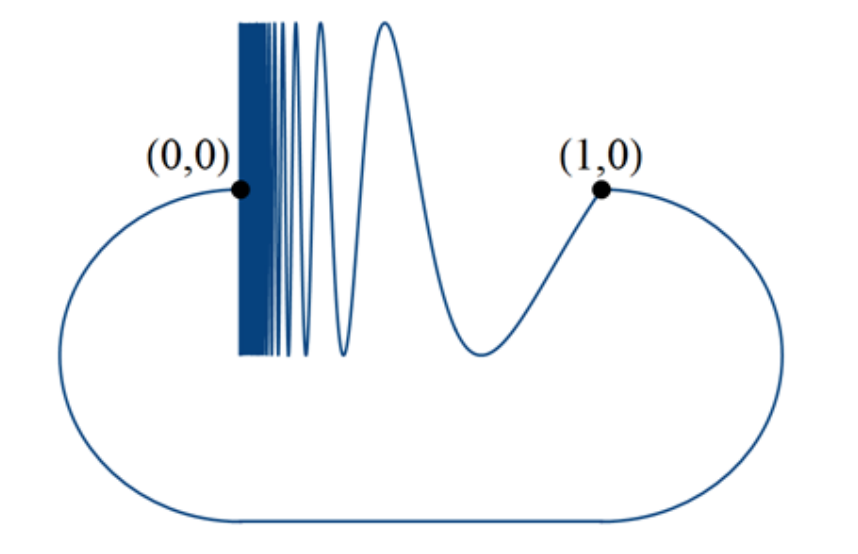
\includegraphics[width = 0.5\textwidth]{2.png}
    \caption{}
    \label{fig:fig2}
\end{figure}
Thus, $X$ is the union of the three sets: $\setb{ \paren{ x , \sin \frac{\pi}{x} } \, \middle| \, 0 \leq x \leq 1 }$, $\setb{ (0,y) \, \middle| \, -1 \leq y \leq 1 }$, and a curved arc from $(0,0)$ to $(1,0)$.
\subsection{Problem 7}
Prove or disprove the following.
\begin{enumerate}[(i)]
    \item $X$ is path connected.
    \item $X$ is locally connected.
    \item $X$ is compact.
\end{enumerate}
\begin{proof}[Answer]
    \noindent
    \begin{enumerate}[(i)]
        \item False. See spring 1998, Problem 2b).
        \item 
        \item True. Since $X$ is closed, it suffices to show that $X$ is bounded. Since we could draw $X$ on a piece of paper, it is bounded. Hence $X$ is compact.
    \end{enumerate}
\end{proof}
\subsection{Problem 8}
\begin{enumerate}[(i)]
    \item Determine the fundamental group $\pi_1(X,(0,0))$.
    \item Sketch a connected double covering of $X$.
    \item State the covering space classification theorem, and explain why parts (i) and (ii) of this question are consistent with the theorem.
\end{enumerate}
\begin{proof}[Answer]
    
\end{proof}
\newpage
\section{Spring 2020 [Answered]}
Answer exactly six of the eight questions.
\subsection{Problem 1}
Let $X$ be a compact metric space. Prove that there exists a finite set of points $x_1 , \dotsc , x_n$ such that every point in $X$ is distance less than 3 from some $x_i$, and $d \paren{ x_i , x_j } \geq 1$ for any $i \neq j$.
\begin{proof}[Answer]
    Recall that a compact metric space is complete, so by Problem 2, $X$ has a finite $\epsilon$-net for $\epsilon = 1$.
\end{proof}
\subsection{Problem 2 \texorpdfstring{\cite{Rudin}}{}}
Suppose $X$ is a metric space such that every sequence in $X$ has a Cauchy subsequence. Prove that $X$ can be covered by finitely many balls of radius 1.
\begin{proof}[Answer]
    We do this in general for an arbitrary $\epsilon$-net. We create a finite $\epsilon$-net for $X$ inductively: Pick $x_1 \in X$, and if for some $n \in \z^+$ the collection of distinct points $\setb{ x_1 , \dotsc , x_n }$ is not a finite $\epsilon$-net for $X$, pick $x_{n+1} \in X$ such that $d \paren{ x_m , x_{n+1} } \geq \epsilon$ for all $1 \leq m \leq n$. We claim that this process must terminate, otherwise we obtain a sequence $\setb{ x_n }_{n = 1}^{\infty}$ such that for all $m , n \in \z^+$, $d \paren{ x_m , x_n } \geq \epsilon$. Thus $\setb{ x_n }_{n = 1}^{\infty}$ cannot have a Cauchy subsequence, which contradicts the condition on $X$. Therefore $X$ has a finite $\epsilon$-net.
\end{proof}
\subsection{Problem 3 \texorpdfstring{\cite{Munkres,Leon}}{}}
Prove that $S^2$ is homeomorphic to a quotient space of $S^1 \times [0,1]$. (You can use any theorems you want, as long as you state them clearly.)
\begin{proof}[Answer]
    Write $X := S^1 \times [0,1]$ as 
    \[
        \setb{ \paren{ \cos \theta , \sin \theta , z } \in \real^3 \, \middle| \, 0 \leq \theta < 2\pi , 0 \leq z \leq 1 }.
    \]
    Let $\sim$ be an equivalence relation on $X$ where 
    \[
        \paren{ \cos \theta , \sin \theta , z } \sim \paren{ \cos \theta' , \sin \theta' , z' }
    \]
    if and only if $z = z' = 0$ or $z = z' = 1$. Let $p$ be the quotient map from $X$ to the set of equivalence classes $X^*$ under $\sim$. We claim that $X^* \cong S^2$. To do this, we quote the following theorem:
    \begin{theorem}
        Let $p : X \to Y$ be a quotient map. Let $Z$ be a space and let $g : X \to Z$ be a map that is constant on each set $\inv{p} \paren{ \setb{ y } }$. Then $g$ induces a map $f : Y \to Z$ such that $f \circ p = g$. $f$ is a homeomorphism if and only if $g$ is a quotient map. 
        \[
            \begin{tikzcd}
                X \arrow[d,"p"',twoheadrightarrow] \arrow[dr,"g",twoheadrightarrow]\\
                Y \arrow[r,"f"',dashed] & Z
            \end{tikzcd}
        \]
    \end{theorem}
    Let $g : S^1 \times [0,1] \to S^2$ be given by 
    \[
        g \paren{ \cos \theta , \sin \theta , z } := \paren{ \sin \paren{ \pi z } \cos \theta , \sin \paren{ \pi z } \sin \theta , \cos \paren{ \pi z } }.
    \]
    From Calculus, $g \paren{ \cos \theta , \sin \theta , z }$ is a parametrization of $S^2$ in $\real^3$, and so $g$ is continuous and surjective. Next, we show that $g$ is constant on the equivalence classes. For $0 \leq \theta < 2\pi$, $0 < z < 1$, $\sqbrack{ \paren{ \cos \theta , \sin \theta , z } }$ consists of a single element, and so $g$ is constant on $\sqbrack{ \paren{ \cos \theta , \sin \theta , z } }$. For any $0 \leq \theta < 2\pi$, we have 
    \begin{align*}
        g \paren{ \cos \theta , \sin \theta , 0 } & = \paren{ \sin \paren{ 0 } \cos \theta , \sin \paren{0} \sin \theta , \cos \paren{0} } \\
        & = (0,0,1), \\
        g \paren{ \cos \theta , \sin \theta , 1 } & = \paren{ \sin \paren{ \pi } \cos \theta , \sin \paren{\pi} \sin \theta , \cos \paren{\pi} } \\
        & = (0,0,-1).
    \end{align*}
    Thus $g$ is constant on the equivalence classes of $X$. Lastly, we show that $g$ is a closed map; since $g$ is already continuous and surjective, this shows that $g$ is a quotient map. Let $C \subseteq X$ be closed. Then as $X$ is compact, $C$ is also compact. By continuity of $g$, $g(C)$ is compact in $S^2$. Since $S^2$ is Hausdorff, $g(C)$ is closed, and so $g$ is a closed map. Thus by the theorem, there exists a homeomorphism $f : X^* \xlongrightarrow{\sim} S^2$ such that $f \circ p = g$. Therefore $S^2$ is homeomorphic to a quotient of $S^1 \times [0,1]$.
\end{proof}
\subsection{Problem 4}
A topological space is called \ita{separable} if it has a countable dense subset. Prove that the product of a countable collection of separable topological spaces is separable.
\begin{proof}[Answer]
    Let $X := \prod\limits_{n = 1}^{\infty} X_n$ have the product topology, where each $X_n$ is separable, with countable dense subset $D_n$. 
    \[Y:=\prod\limits_{n=1}^{\infty}D_n,\]
    and fix $\mathbf{y}=(y_1,y_2,\dotsc)\in Y$. For each $N\in\z^+$, let 
    \[S_N:=\{\mathbf{x}\in Y\mid x_n=y_n\text{ for all but finitely many }n\in\z^+\},\]
    and let 
    \[S:=\bigcup\limits_{N=1}^{\infty}S_N.\]
    We claim that $S$ is countable and dense in $X$. Note that for each $N\in\z^+$, $S_N$ is countable, as
    \[S_N=\prod\limits_{n=1}^ND_n\times\prod\limits_{n=N+1}^{\infty}\{y_n\},\]
    and so $S$ is the countable union of countable sets, which is countable. To show that $S$ is dense, it suffices to show that $S$ intersects every non-empty basis element non-trivially. Recall that an arbitrary basis element $B$ of $X$ is of the form
    \[B=\prod\limits_{n=1}^mU_n\times\prod\limits_{n=m+1}^{\infty}X_n\]
    for some $m\in\z^+$, where $U_n\subseteq X_n$ is open for all $1\leq n\leq m$. Then
    \begin{align*}
        S_m\cap B&=\left(\prod\limits_{n=1}^ND_n\times\prod\limits_{n=N+1}^{\infty}\{y_n\}\right)\times\left(\prod\limits_{n=1}^mU_n\times\prod\limits_{n=m+1}^{\infty}X_n\right)\\
        &=\left(\prod\limits_{n=1}^m D_n\cap U_n\right)\times\left(\prod\limits_{n=m+1}^{\infty}\{y_n\}\cap X_n\right) \\
        &=\left(\prod\limits_{n=1}^m D_n\cap U_n\right)\times\left(\prod\limits_{n=m+1}^{\infty}\{y_n\}\right).
    \end{align*}
    As $D_n$ is dense in $X_n$, $D_n\cap U_n\neq\varnothing$ for all $1\leq n\leq m$. Hence $S_m\cap B\neq\varnothing$, and so $S\cap B\neq\varnothing$. Thus $S$ is dense in $X$.
    
    Therefore $X$ has a dense and countable subset, and so is separable.
\end{proof}
\subsection{Problem 5}
Let $(X,d)$ be a metric space, and fix a point $x_0 \in X$. Let $\rho$ be a new metric given by $\rho(x,y) = d \paren{ x , x_0 } + d \paren{ y , x_0 }$ if $x \neq y$, and $\rho(x,x) = 0$. Verify that $\rho$ is a metric, and prove that $(X,\rho)$ is complete.
\begin{proof}[Answer]
    First, we verify that $\rho$ is a metric.
    \begin{enumerate}
        \item Since $d$ is a metric,
        \[
            d \paren{ x, x_0 } + d \paren{ y , x_0 } \geq 0,
        \]
        and so $\rho(x,y) \geq 0$ for all $x , y \in X$. By definition of $\rho$, $\rho(x,y) = 0$ if and only if $x = y$.
        \item Since $(\real,+)$ is an abelian group, $\rho(x,y) = \rho(y,x)$ for all $x,y \in X$.
        \item Let $x , y , z \in X$. Note that if any of $x$, $y$, or $z$ are equal, then 
        \[
            \rho(x,y) \leq \rho(x,z) + \rho(z,y)
        \]
        will trivially hold, so assume that all of $x$, $y$, and $z$ are distinct. Then 
        \begin{align*}
            \rho(x,y) & = d \paren{ x , x_0 } + d \paren{ y , x_0 } \\
            & \leq d \paren{ x , x_0 } + d \paren{ z , x_0 } +  d \paren{ y , x_0 } + d \paren{ z , x_0 } \\
            & = \rho(x,z) + \rho(y,z) \\
            & = \rho(x,z) + \rho(z,y).
        \end{align*}
        Therefore $\rho$ is a metric.
    \end{enumerate}
    Now, let $\setb{ x_n }_{n = 1}^{\infty}$ be a Cauchy sequence. Then for all $\epsilon > 0$, there exists $N \in \z^+$ such that for all $n , m > N$, 
    \[
        \rho \paren{ x_n , x_m } \leq d \paren{ x_n , x_0 } + d \paren{ x_m , x_0 } < \epsilon.
    \]
    Then for all $n , m > N$, 
    \begin{align*}
        \rho \paren{ x_n , x_0 } & \leq d \paren{ x_n , x_0 } + d \paren{ x_0 , x_0 } \\
        & = d \paren{ x_n , x_0 } \\
        & \leq d \paren{ x_n , x_0 } + d \paren{ x_m , x_0 } \\
        & \leq \epsilon.
    \end{align*}
    Therefore $\setb{ x_n }_{n = 1}^{\infty}$ converges, and it converges to $x_0$. Therefore $(X,\rho)$ is a complete metric space.
\end{proof}
\subsection{Problem 6}
Prove that the product of two regular spaces is regular.
\begin{proof}[Answer]
    See Fall 2014, Problem 7(ii).
\end{proof}
\subsection{Problem 7 \texorpdfstring{\cite{Arthur}}{}}
A topological space is called \ita{totally disconnected} if every pair of points is contained in a pair of disjoint open sets whose union is the whole space. Prove that every countable metric space is totally disconnected.
\begin{proof}[Answer]
    Note that what this problem calls totally disconnected is actually the definition of \underline{totally separated}. A totally disconnected space is one where the only connected subsets are singletons. Note that a totally separated space is totally disconnected: let $A \subseteq X$ contain at least two points. Pick $x , y \in A$, then there exists $U , V \subset X$ open and disjoint such that $x \in U$, $y \in V$, and $U \cup V = X$. Then $U \cap A$ and $V \cap A$ are open in $A$ and disjoint, $x \in U \cap A$, $y \in U \cap B$, and 
    \begin{align*}
        \paren{ U \cap A } \cup \paren{ V \cap A } & = \paren{ U \cup V } \cap A \\
        & = X \cap A \\
        & = A.
    \end{align*}
    Thus $A$ has a separation, and so is not connected. 
    
    However, it turns out that a totally disconnected space may not be totally separated. We will not explore an example here, but because of this fact, we will only use the property of totally separated from here on out. Furthermore, the question is inapplicable if $X$ only contains a single element, so assume that $|X| \geq 2$.
    
    Now, let $(X,d)$ be a countable metric space with $|X| \geq 2$. Fix $x_0 \in X$, and let $f : X \to \real$ be given by $f(x) := d \paren{ x_0 , x }$. Note that $f$ is continuous (in fact Lipschitz) and that $f(X) \subset [0,\infty)$ is countable (since $X$ itself is countable). Thus there exists $r > 0$ such that $r \notin f(X)$, so the set 
    \[
        \inv{f} \paren{ \setb{ r } } = \setb{ x \in X \, \middle| \, d \paren{ x_0 , x } = r }
    \]
    is empty. Then 
    \[
        B_r \sqbrack{ x_0 } = B_r \paren{ x_0 } \uplus \inv{f} \paren{ \setb{ r } } = B_r \paren{ x_0 }.
    \]
    Since 
    \[
        B_r \paren{ x_0 } \subseteq \overline{ B_r \paren{ x_0 } } \subseteq B_r \sqbrack{ x_0 },
    \]
    $B_r \paren{ x_0 } = \overline{B_r \paren{ x_0 }}$, and so $B_r \paren{ x_0 }$ is clopen. 
    
    Then using the above procedure, for any two distinct points $x , y \in X$, there exists $0 < r < d(x,y)$ such that $B_r(x)$ is clopen. Then $X \setminus B_r(x)$ is also clopen and contains $y$. Therefore $(X,d)$ is totally separated. 
\end{proof}
\subsection{Problem 8}
Prove that the free group on two generators has a subgroup isomorphic to the free group on $n$ generators for any $n$. You can use any theorems from the theory of covering spaces. You can also state without proof the fundamental group of any spaces you use in your proof.
\begin{proof}[Answer]
    
\end{proof}
\newpage
\section{Extra Stuff}
\begin{enumerate}
    \item A compact metric space $(X,d)$ is complete. \cite{Berge}
    \begin{proof}
        Let $\setb{ x_n }_{n = 1} \subseteq X$ be a Cauchy sequence. Since $X$ is compact, $\setb{ x_n }_{n = 1}$ has a convergent subsequence. Thus $\setb{ x_n }_{n = 1}$ also converges and so $X$ is complete.
    \end{proof}
    \item Show that $\q$ is not locally compact.
    \begin{proof}[Answer]
        Recall that $X$ is locally compact if for all $x \in X$, there exists a compact subspace $K \subseteq X$ that contains a neighborhood of $X$. To show that $\q$ is not locally compact, it suffices to show that none of its basis elements are contained in a compact subspace. Recall that a basis element of the subspace topology on $\q$ is of the form $(a,b) \cap \q$ for some $a,b \in \real$, $a<b$. Let $a < r < b$ be an irrational number, then since $\q$ is dense in $\real$, there exists a sequence $\setb{ x_n }_{n = 1}^{\infty} \subseteq (a,b) \cap \q$ that converges to $r$. Suppose that $(a,b) \cap \q$ is contained in a compact subspace $K \subseteq \q$. Then there exists a subsequence $\setb{ x_{n_k} }_{k=1}^{\infty} \subseteq \setb{ x_n }_{n=1}^{\infty}$ converging to some $x_0 \in K$. But since $\setb{ x_n }_{n = 1}^{\infty}$ converges in $(a,b)$, $\setb{ x_{n_k} }_{k=1}^{\infty}$ must also converge in $(a,b)$ to $r$. Thus $x_0 = r$, which contradicts $r$ being irrational. Therefore no such compact subspace $K \subseteq \q$ exists and so $\q$ is not locally compact.
    \end{proof}
\end{enumerate}
\newpage
\phantomsection
\addcontentsline{toc}{section}{References}
\begin{thebibliography}{99}
    \bibitem{step} Brandsma, Henno (\url{https://math.stackexchange.com/users/4280/henno-brandsma}). Proof of theorem 26.15 in ``General Topology'' by Willard. Mathematics Stack Exchange. Accessed 24 June 2020. \url{https://math.stackexchange.com/questions/973733}.
    \bibitem{Ricky} Lee, Ricky.
    \bibitem{Scott} Scott, Brian M. (\url{https://math.stackexchange.com/users/12042/brian-m-scott}). Compactness and Strictly Finer Topologies. Mathematics Stack Exchange. Accessed 28 June 2020. \url{https://math.stackexchange.com/questions/328923}.
    \bibitem{Munkres} Munkres, James R. \ita{Topology, $2^{nd}$ Ed.} Pearson, 2000.
    \bibitem{Desmos} Desmos Online Graphing Calculator.
    \bibitem{stm} k.stm. (\url{https://math.stackexchange.com/users/42242/k-stm}). How to prove the continuity of the metric function? Mathematics Stack Exchange. Accessed 13 July 2020. \url{https://math.stackexchange.com/questions/287285}.
    \bibitem{Jacob} Cornejo, Jacob.
    \bibitem{DF} Dummit, David S. and Richard M. Foote. \ita{Abstract Algebra, $3^{rd}$ Ed.} John Wiley \& Sons, Inc. 2004.
    \bibitem{Rico} Vicente, Rico.
    \bibitem{Leon} Kim, Leon.
    \bibitem{proper} user99914 (url unavailable). Are all proper maps continuous. Accessed 15 July 2020. \url{https://math.stackexchange.com/questions/2508659/}.
    \bibitem{Blair} Blair, Ryan. MATH 550 Course Notes. Fall 2018.
    \bibitem{Berge} Berge, Claude. \ita{Topological Spaces}. Translated by E. M. Patterson. Dover Publications, Inc. 1997.
    \bibitem{Pilar} Orellana, Pilar.
    \bibitem{Schnell} Schnell, Christian. \ita{MAT 530: Geometry and Topology I Course Notes 2014}. Accessed 04 Septebmer 2020. \url{https://www.math.stonybrook.edu/~cschnell/pdf/notes/mat530.pdf}.  
    \bibitem{Rudin} Rudin, Walter. \ita{Principles of Mathematical Analysis, $3^{rd}$ Ed.} McGraw-Hill Education. 1976.
    \bibitem{Arthur} Arthur (\url{https://math.stackexchange.com/users/15500/arthur}). Proving that every countable metric space is disconnected? [duplicate]. Accessed 01 September 2020. \url{https://math.stackexchange.com/questions/504588}.
    \bibitem{Hatcher} Hatcher, Allen.
    \ita{Algebraic Topology}. 2001. \url{http://pi.math.cornell.edu/~hatcher/AT/AT.pdf}
\end{thebibliography}
\end{document}